%        روش اجرا.: 2 بار F1 ، 2 بار  F11(به منظور تولید مراجع) ، دوبار Ctrl+Alt+I (به منظور تولید نمایه) و دو بار F1 -------> مشاهده Pdf
%%%%%%%%%%%%%%%%%%%%%%%%%%%%%%%%%%%%%%%%%%%%%%%%%%%%%%
%   TeXstudio as your IDE
%%  برای compile در TeXstudio تنها کافی است منوی Options->Configure TeXstudio را زده و در پنجره Configure TeXstudio در بخش Build گزینه Default Compiler را به XeLaTeX تغییر دهید. سند شما به راحتی compile خواهد شد.
%   F1 & F5 : Build & view
%   F6      : Compile
%   F7      : View
%   --------------
%%%%%%%%%%%%%%%%%%%%%%%%%%%%%%%%%%%%%%%%%%%%%%%%%%%%%%
%        اگر قصد نوشتن رساله دکتری را دارید، در خط زیر به جای msc،
%      کلمه phd را قرار دهید. کلیه تنظیمات لازم، به طور خودکار، اعمال می‌شود.
%%\TEX TS-program = XeLaTeX
\documentclass[oneside,bsc,12pt]{AUTthesis}
%       فایل commands.tex را حتماً به دقت مطالعه کنید؛ چون دستورات مربوط به فراخوانی بسته زی‌پرشین 
%       و دیگر بسته‌ها و ... در این فایل قرار دارد و بهتر است که با نحوه استفاده از آنها آشنا شوید. توجه شود برای نسخه نهایی پایان‌نامه حتماً hyperref را 
%        غیرفعال کنید.

\usepackage{bigfoot}
% در این فایل، دستورها و تنظیمات مورد نیاز، آورده شده است.
%-------------------------------------------------------------------------------------------------------------------
% در ورژن جدید زی‌پرشین برای تایپ متن‌های ریاضی، این سه بسته، حتماً باید فراخوانی شود.
\usepackage{amsthm,amssymb,amsmath,amsfonts}
\usepackage[numbers,sort&compress]{natbib}
\usepackage[export]{adjustbox}
\usepackage{xstring}

% بسته‌ای برای تنطیم حاشیه‌های بالا، پایین، چپ و راست صفحه
\usepackage[top=30mm, bottom=30mm, left=25mm, right=30mm]{geometry}
% بسته‌‌ای برای ظاهر شدن شکل‌ها و تصاویر متن
\usepackage{graphicx}
\usepackage{color}
%بسته‌ای برای تنظیم فاصله عمودی خط‌های متن
\usepackage{setspace}
\usepackage{titletoc}
\usepackage{tocloft}
\usepackage[labelsep=space]{caption}
%با فعال کردن بسته زیر فوت‌نوت‌ها در هر صفحه ریست می‌شوند. حالت پیش‌فرض آن ریست شدن در هر فصل می‌باشد.
\usepackage[stable]{footmisc}
\usepackage{enumitem}
%\usepackage{titlesec}
% بسته‌ و دستوراتی برای ایجاد لینک‌های رنگی با امکان جهش
\usepackage[pagebackref=false,colorlinks,linkcolor=blue,citecolor=red]{hyperref}
\usepackage[nameinlink]{cleveref}%capitalize,,noabbrev
 \AtBeginDocument{%
    \crefname{equation}{رابطه}{equations}%
    \crefname{chapter}{فصل}{chapters}%
    \crefname{section}{بخش}{sections}%
    \crefname{appendix}{پیوست}{appendices}%
    \crefname{enumi}{مورد}{items}%
    \crefname{footnote}{زیرنویس}{footnotes}%
    \crefname{figure}{شکل}{figures}%
    \crefname{table}{جدول}{tables}%
    \crefname{theorem}{قضیه}{theorems}%
    \crefname{lemma}{لم}{lemmas}%
    \crefname{corollary}{نتیجه}{corollaries}%
    \crefname{proposition}{گزاره}{propositions}%
    \crefname{definition}{تعریف}{definitions}%
    \crefname{result}{نتیجه}{results}%
    \crefname{example}{مثال}{examples}%
    \crefname{remark}{نکته}{remarks}%
    \crefname{note}{یادداشت}{notes}%
}
% چنانچه قصد پرینت گرفتن نوشته خود را دارید، خط بالا را غیرفعال و  از دستور زیر استفاده کنید چون در صورت استفاده از دستور زیر‌‌، 
% لینک‌ها به رنگ سیاه ظاهر خواهند شد که برای پرینت گرفتن، مناسب‌تر است
%\usepackage[pagebackref=false]{hyperref}
% بسته‌ لازم برای تنظیم سربرگ‌ها
\usepackage{fancyhdr}
% بسته‌ای برای ظاهر شدن «مراجع»  در فهرست مطالب
\usepackage[nottoc, notlof, notlot]{tocbibind}
% دستورات مربوط به ایجاد نمایه
\usepackage{makeidx,multicol}
\setlength{\columnsep}{1.5cm}
% \renewcommand{\thefootnote}{{\arabic{footnote}}}
%%%%%%%%%%%%%%%%%%%%%%%%%%
\usepackage{verbatim}
\makeindex
\usepackage{sectsty}
% فراخوانی بسته زی‌پرشین و تعریف قلم فارسی و انگلیسی
\usepackage{xepersian}%[extrafootnotefeatures]
\ExplSyntaxOn
\cs_set_eq:NN
\etex_iffontchar:D
\tex_iffontchar:D
\cs_undefine:N \c_one
\int_const:Nn \c_one { 1 } 
\ExplSyntaxOff

\SepMark{-}
%حتماً از تک لایو 2014 استفاده کنید.
\settextfont[Scale=1.2]{B-NAZANIN.TTF}
\setlatintextfont{times new roman.ttf}
\renewcommand{\labelitemi}{$\bullet$}
%%%%%%%%%%%%%%%%%%%%%%%%%%
% چنانچه می‌خواهید اعداد در فرمول‌ها، انگلیسی باشد، خط زیر را غیرفعال کنید.
%در غیر اینصورت حتماً فونت PGaramond را نصب کنید.
% \setdigitfont[Scale=1.1]{XB Yas}%%Yas
%%%%%%%%%%%%%%%%%%%%%%%%%%
% تعریف قلم‌های فارسی اضافی برای استفاده در بعضی از قسمت‌های متن
\defpersianfont\nastaliq[Scale=2]{IranNastaliq.ttf}
\defpersianfont\chapternumber[Scale=3]{B-NAZANIN.TTF}
% \chapterfont{\centering}%
%%%%%%%%%%%%%%%%%%%%%%%%%% 
% دستوری برای تغییر نام کلمه «اثبات» به «برهان»
\renewcommand\proofname{\textbf{برهان}}

% دستوری برای تغییر نام کلمه «کتاب‌نامه» به «منابع و مراجع«
\renewcommand{\bibname}{منابع و مراجع}


% Headings for every page of ToC, LoF and Lot
\setlength{\cftbeforetoctitleskip}{-1.2em}
\setlength{\cftbeforelottitleskip}{-1.2em}
\setlength{\cftbeforeloftitleskip}{-1.2em}
\setlength{\cftaftertoctitleskip}{-1em}
\setlength{\cftafterlottitleskip}{-1em}
\setlength{\cftafterloftitleskip}{-1em}
%%\makeatletter
%%%%\renewcommand{\l@chapter}{\@dottedtocline{1}{1em\bfseries}{1em}}
%%%%\renewcommand{\l@section}{\@dottedtocline{2}{2em}{2em}}
%%%%\renewcommand{\l@subsection}{\@dottedtocline{3}{3em}{3em}}
%%%%\renewcommand{\l@subsubsection}{\@dottedtocline{4}{4em}{4em}}
%%%%\makeatother


\newcommand\tocheading{\par عنوان\hfill صفحه \par}
\newcommand\lofheading{\hspace*{.5cm}\figurename\hfill صفحه \par}
\newcommand\lotheading{\hspace*{.5cm}\tablename\hfill صفحه \par}

\renewcommand{\cftchapleader}{\cftdotfill{\cftdotsep}}
\renewcommand{\cfttoctitlefont}{\hspace*{\fill}\LARGE\bfseries}%\Large
\renewcommand{\cftaftertoctitle}{\hspace*{\fill}}
\renewcommand{\cftlottitlefont}{\hspace*{\fill}\LARGE}%\Large
\renewcommand{\cftafterlottitle}{\hspace*{\fill}}
\renewcommand{\cftloftitlefont}{\hspace*{\fill}\LARGE\bfseries}
\renewcommand{\cftafterloftitle}{\hspace*{\fill}}

%%%%%%%%%%%%%%%%%%%%%%%%%%
% تعریف و نحوه ظاهر شدن عنوان قضیه‌ها، تعریف‌ها، مثال‌ها و ...
%برای شماره گذاری سه تایی قضیه ها
\theoremstyle{definition}
\newtheorem{definition}{تعریف}[section]
\newtheorem{remark}[definition]{نکته}
\newtheorem{note}[definition]{یادداشت}
\newtheorem{example}[definition]{نمونه}
\newtheorem{question}[definition]{سوال}
\newtheorem{remember}[definition]{یاداوری}
\theoremstyle{theorem}
\newtheorem{theorem}[definition]{قضیه}
\newtheorem{lemma}[definition]{لم}
\newtheorem{proposition}[definition]{گزاره}
\newtheorem{corollary}[definition]{نتیجه}
%%%%%%%%%%%%%%%%%%%%%%%%
%%%%%%%%%%%%%%%%%%%
%%% برای شماره گذاری چهارتایی قضیه ها و ...
%%\newtheorem{definition1}[subsubsection]{تعریف}
%%\newtheorem{theorem1}[subsubsection]{قضیه}
%%\newtheorem{lemma1}[subsubsection]{لم}
%%\newtheorem{proposition1}[subsubsection]{گزاره}
%%\newtheorem{corollary1}[subsubsection]{نتیجه}
%%\newtheorem{remark1}[subsubsection]{نکته}
%%\newtheorem{example1}[subsubsection]{مثال}
%%\newtheorem{question1}[subsubsection]{سوال}

%%%%%%%%%%%%%%%%%%%%%%%%%%%%

% دستورهایی برای سفارشی کردن صفحات اول فصل‌ها
\makeatletter
\newcommand\mycustomraggedright{%
 \if@RTL\raggedleft%
 \else\raggedright%
 \fi}
\def\@makechapterhead#1{%
\thispagestyle{style1}
\vspace*{20\p@}%
{\parindent \z@ \mycustomraggedright
\ifnum \c@secnumdepth >\m@ne
\if@mainmatter

\centering\bfseries{\Huge \@chapapp}\small\space {\chapternumber\thechapter}
\thispagestyle{empty}
\par\nobreak
\vskip 0\p@
\fi
\fi
\interlinepenalty\@M 
\Huge \bfseries #1\par\nobreak
\vskip 120\p@

}

\newpage}
\bidi@patchcmd{\@makechapterhead}{\thechapter}{\tartibi{chapter}}{}{}
\bidi@patchcmd{\chaptermark}{\thechapter}{\tartibi{chapter}}{}{}
\makeatother

\pagestyle{fancy}
\renewcommand{\chaptermark}[1]{\markboth{\chaptername~\tartibi{chapter} - #1}{}}

\fancypagestyle{style1}{
\fancyhf{} 
\fancyfoot[c]{\thepage}
\fancyhead[R]{\leftmark}%
\renewcommand{\headrulewidth}{1.2pt}
}


\fancypagestyle{style2}{
\fancyhf{}
\fancyhead[R]{چکیده}
\fancyfoot[C]{\thepage{}}
\renewcommand{\headrulewidth}{1.2pt}
}

\fancypagestyle{style3}{%
  \fancyhf{}%
  \fancyhead[R]{فهرست نمادها}
  \fancyfoot[C]{\thepage}%
  \renewcommand{\headrulewidth}{1.2pt}%
}

\fancypagestyle{style4}{%
  \fancyhf{}%
  \fancyhead[R]{فهرست جداول}
  \fancyfoot[C]{\thepage}%
  \renewcommand{\headrulewidth}{1.2pt}%
}

\fancypagestyle{style5}{%
  \fancyhf{}%
  \fancyhead[R]{فهرست اشکال}
  \fancyfoot[C]{\thepage}%
  \renewcommand{\headrulewidth}{1.2pt}%
}

\fancypagestyle{style6}{%
  \fancyhf{}%
  \fancyhead[R]{فهرست مطالب}
  \fancyfoot[C]{\thepage}%
  \hypersetup{linkcolor=black, citecolor=black}
  \renewcommand{\headrulewidth}{1.2pt}%
}

\fancypagestyle{style7}{%
  \fancyhf{}%
  \fancyhead[R]{نمایه}
  \fancyfoot[C]{\thepage}%
  \renewcommand{\headrulewidth}{1.2pt}%
}

\fancypagestyle{style8}{%
  \fancyhf{}%
  \fancyhead[R]{منابع و مراجع}
  \fancyfoot[C]{\thepage}%
  \renewcommand{\headrulewidth}{1.2pt}%
}
\fancypagestyle{style9}{%
  \fancyhf{}%
  \fancyhead[R]{واژه‌نامه‌ی فارسی به انگلیسی}
  \fancyfoot[C]{\thepage}%
  \renewcommand{\headrulewidth}{1.2pt}%
}
%


%دستور حذف نام لیست تصاویر و لیست جداول از فهرست مطالب
\newcommand*{\BeginNoToc}{%
  \addtocontents{toc}{%
    \edef\protect\SavedTocDepth{\protect\the\protect\value{tocdepth}}%
  }%
  \addtocontents{toc}{%
    \protect\setcounter{tocdepth}{10}%
  }%
}
\newcommand*{\EndNoToc}{%
  \addtocontents{toc}{%
    \protect\setcounter{tocdepth}{\protect\SavedTocDepth}%
  }%
}
\newcounter{savepage}
\renewcommand{\listfigurename}{فهرست اشکال}
\renewcommand{\listtablename}{فهرست جداول}
%\renewcommand\cftsecleader{\cftdotfill{\cftdotsep}}
%%%%%%%%%%%%%%%%%%%%%%%%%%%%%
%%%%%%%%%%%%%%%%%%%%%%%%%%%%

\begin{document}
\baselineskip=.75cm
\linespread{1.75}
%% -!TEX root = AUTthesis.tex
% در این فایل، عنوان پایان‌نامه، مشخصات خود، متن تقدیمی‌، ستایش، سپاس‌گزاری و چکیده پایان‌نامه را به فارسی، وارد کنید.
% توجه داشته باشید که جدول حاوی مشخصات پروژه/پایان‌نامه/رساله و همچنین، مشخصات داخل آن، به طور خودکار، درج می‌شود.
%%%%%%%%%%%%%%%%%%%%%%%%%%%%%%%%%%%%
% دانشکده، آموزشکده و یا پژوهشکده  خود را وارد کنید
\faculty{دانشکده مهندسی کامپیوتر}
% گرایش و گروه آموزشی خود را وارد کنید
\department{}
% عنوان پایان‌نامه را وارد کنید
\fatitle{هدایت پهپاد با علائم دست مبتنی بر بینایی ماشین}
% نام استاد(ان) راهنما را وارد کنید
\firstsupervisor{دکتر مهدی جوانمردی }
\secondsupervisor{}
% نام استاد(دان) مشاور را وارد کنید. چنانچه استاد مشاور ندارید، دستور پایین را غیرفعال کنید.
%\firstadvisor{نام کامل استاد مشاور}
%\secondadvisor{استاد مشاور دوم}
% نام نویسنده را وارد کنید
\name{سارا }
% نام خانوادگی نویسنده را وارد کنید
\surname{تاجرنیا}
%%%%%%%%%%%%%%%%%%%%%%%%%%%%%%%%%%
\thesisdate{خرداد ۱۴۰۳}


% چکیده پایان‌نامه را وارد کنید
\fa-abstract{پهپادهای تجاری که به عنوان هواپیما‌های بدون سرنشین\LTRfootnote{Unmanned Aerial Vehicles} 
نیز شناخته می‌شوند، به سرعت در حال رایج شدن هستند. این پهپاد‌ها در زمینه‌های مختلف مانند نظارت بر رویدادهای ورزشی، حمل و نقل تجهیزات
 و کالاهای اضطراری، فیلمبرداری، عکس‌برداری هوایی و ... مورد استفاده قرار می‌گیرند.
  \\
هدف این پروژه توسعه سیستمی است که بتوان با استفاده از آن, از حرکات دست به عنوان روشی برای کنترل پرواز پهپاد‌ها استفاده کرد.
بدین صورت که با استفاده از روش‌های مبتنی بر بینایی ماشین\LTRfootnote{Computer Vision}، روشی بصری برای ارتباط بدون عامل, بین پهپاد و اپراتور آن ایجاد کرد.
 روش‌های مبتنی بر بینایی ماشین با استفاده از دوربین هواپیما‌های بدون سرنشین که تصاویر اطراف را گرفته و پس
 از تحلیل تصاویر و تشخیص الگوی دست، اطلاعات معناداری از آن را استخراج می‌کنند. ساختار این پروژه از دو ماژول
 اصلی تشخیص حرکت دست\LTRfootnote{Hand Detection}
 و دستور به هواپیمای بدون سرنشین تشکیل شده است. برای ماژول اول از یک روش مبتنی بر
 یادگیری عمیق\LTRfootnote{Deep Learning}
  استفاده شده است که در فصل‌های بعدی به توضیح آن می‌پردازیم. ماژول دوم نیز وظیفه ارتباط با پهپاد را بر عهده دارد که نتایج سیستم تشخیص را برای پهپاد ارسال می‌کند.
 نتایج به دست آمده گواه بر عملکرد صحیح همراه با دقت بالای این سیستم است.
 }
% کلمات کلیدی پایان‌نامه را وارد کنید
\keywords{
    پهپاد‌ها، حرکات دست، شبکه‌‌های عصبی پیچشی\LTRfootnote{Convolutional Neural Network(CNN)}
    ، حافظه طولانی کوتاه مدت\LTRfootnote{Long Short-Term Memory(LSTM)}، شبکه عصبی بازگشتی\LTRfootnote{Recurrent Neural Network(RNN)}، رابط انسان و پهپاد\LTRfootnote{Human–Drone Interface}
}



\AUTtitle{a}
%%%%%%%%%%%%%%%%%%%%%%%%%%%%%%%%%%
\vspace*{7cm}
\thispagestyle{empty}
\begin{center}
\includegraphics[height=5cm,width=12cm]{besm}
\end{center}
%% -!TEX root = AUTthesis.tex
% در این فایل، عنوان پایان‌نامه، مشخصات خود، متن تقدیمی‌، ستایش، سپاس‌گزاری و چکیده پایان‌نامه را به فارسی، وارد کنید.
% توجه داشته باشید که جدول حاوی مشخصات پروژه/پایان‌نامه/رساله و همچنین، مشخصات داخل آن، به طور خودکار، درج می‌شود.
%%%%%%%%%%%%%%%%%%%%%%%%%%%%%%%%%%%%
% دانشکده، آموزشکده و یا پژوهشکده  خود را وارد کنید
\faculty{دانشکده مهندسی کامپیوتر}
% گرایش و گروه آموزشی خود را وارد کنید
\department{}
% عنوان پایان‌نامه را وارد کنید
\fatitle{هدایت پهپاد با علائم دست مبتنی بر بینایی ماشین}
% نام استاد(ان) راهنما را وارد کنید
\firstsupervisor{دکتر  مهدی جوانمردی}
% \secondsupervisor{}
% نام استاد(دان) مشاور را وارد کنید. چنانچه استاد مشاور ندارید، دستور پایین را غیرفعال کنید.
%\firstadvisor{نام کامل استاد مشاور}
%\secondadvisor{استاد مشاور دوم}
% نام نویسنده را وارد کنید
\name{سارا }
% نام خانوادگی نویسنده را وارد کنید
\surname{تاجرنیا}
%%%%%%%%%%%%%%%%%%%%%%%%%%%%%%%%%%
\thesisdate{خرداد ۱۴۰۳}


\AUTtitle{b}
%%%%%%%%%%%%%%%%%%%%%%%%%%%%%%%%%%

% تاییدیه دفاع
\newpage
\thispagestyle{empty}
%\fontsize{18pt}{19pt}\selectfont

\section*{صفحه فرم ارزیابی و تصویب پایان نامه- فرم تأیید اعضاء كميته دفاع}

\fontsize{12pt}{14pt}\selectfont
%\renewcommand{\baselinestretch}{1.5}
\vspace*{1cm}
   در این صفحه فرم دفاع یا تایید و تصویب پایان نامه موسوم به فرم کمیته دفاع- موجود در پرونده آموزشی- را قرار دهید.
\vspace*{1cm}


\subsection*{نکات مهم:}
 
\begin{itemize}
\item
	نگارش پایان نامه/رساله باید به
	{\color{red}
		زبان فارسی
	}
	و بر اساس آخرین نسخه دستورالعمل و راهنمای تدوین پایان نامه های دانشگاه صنعتی امیرکبیر باشد.(دستورالعمل و راهنمای حاضر)
\item رنگ جلد پایان نامه/رساله چاپي كارشناسي، كارشناسي ارشد و دكترا  بايد به ترتيب مشكي، طوسي و سفيد رنگ باشد.  
\item چاپ و صحافی پایان نامه/رساله بصورت
{\color{red}
	پشت و رو(دورو)
}
بلامانع است و انجام آن توصيه مي شود. 
\end{itemize}
%%%%%%%%%%%%%%%%%%%%%%%%%%%%%%%%%%%%%%%%%%%%%%%%%%%%%%%%%%%%%%%%%%%%%%%%%%%%%%%%%%%%%%%%%%%%%%%%%%
%%%%%%%%%%%%%%%%%%%%%%%%%%%%%%%%%%%%%%%%%%%%%%%%%%%%%%%%%%%%%%%%%%%%%%%%%%%%%%%%%%%%%%%%%%%%%%%%%%
\newpage
\thispagestyle{empty}
\begin{picture}(50,50)
  \put(17,0){
\includegraphics[scale=1.1]{fa-logo}}
  \put(4.5,-13){\footnotesize{دانشگاه صنعتی امیرکبیر}}
  \put(10.5,-27){\footnotesize{(پلی‌تکنیک تهران)}}
  \put(170,30){\bf{به نام خدا}}
  \put(140,-5){\Large\bf{تعهدنامه اصالت اثر}}
  \put(310,0){تاریخ: \datethesis}
\end{picture}

\vspace*{2.5cm}

اينجانب {\bf{\fname\lname}} متعهد می‌شوم که مطالب مندرج در این پایان‌نامه حاصل کار پژوهشی اینجانب تحت نظارت و راهنمایی اساتید دانشگاه صنعتی امیرکبیر بوده و به دستاوردهای دیگران که در این پژوهش از آنها استفاده شده است مطابق مقررات و روال متعارف ارجاع و در فهرست منابع و مآخذ ذکر گردیده است. این پایان‌نامه قبلاً برای احراز هیچ مدرک هم‌سطح یا بالاتر ارائه نگردیده است.

در صورت اثبات تخلف در هر زمان، مدرک تحصیلی صادر شده توسط دانشگاه از درجه اعتبار ساقط بوده و دانشگاه حق پیگیری قانونی خواهد داشت.


کلیه نتایج و حقوق حاصل از این پایان‌نامه متعلق به دانشگاه صنعتی امیرکبیر می‌باشد. هرگونه استفاده از نتایج علمی و عملی، واگذاری اطلاعات به دیگران یا چاپ و تکثیر، نسخه‌برداری، ترجمه و اقتباس از این پایان نامه بدون موافقت کتبی دانشگاه صنعتی امیرکبیر ممنوع است. 
نقل مطالب با ذکر مآخذ بلامانع است.\\
\vspace{2.5cm}


{\centerline {\bf{\fname\lname}}}
\vspace*{.2cm}
{\centerline{امضا}}
%%%%%%%%%%%%%%%%%%%%%%%%%%%%%%%%%
% چنانچه مایل به چاپ صفحات «تقدیم»، «نیایش» و «سپاس‌گزاری» در خروجی نیستید، خط‌های زیر را با گذاشتن ٪  در ابتدای آنها غیرفعال کنید.
% پایان‌نامه خود را تقدیم کنید
% نیایش خود را در فایل زیر بنویسید.
\begin{acknowledgementpage}

\vspace{1.5cm}

{\nastaliq
{
    این پایان نامه را تقدیم می‌کنم به مهربانترين همراهان زندگیم، پدر، مادر، برادران عزیزم که حضورشان همیشه گرما بخش روح من بوده است.
 }}\end{acknowledgementpage}
\newpage
% سپاسگزاری را در فایل زیر بنویسید.
%%%%%%%%%%%%%%%%%%%%%%%%%%%%%%%%%%%%
\newpage\thispagestyle{empty}
% سپاس‌گزاری
{\nastaliq
سپاس‌گزاری
}
\\[2cm]
زندگی دفتری از خاطره هاست،
یك نفر در دل شب،
یك نفر در دل خاک،
یك نفر همدم خوشبختی هاست،
یك نفر همسفر سختی هاست،
چشم تا باز كنیم،
عمرمان می‌گذرد ما همه رهگذریم،
آنچه باقیست فقط خوبیهاست.
\\
تشکر می‌کنم از تمامی عزیزانی که در تمامی مراحل زندگی همراه من بوده اند.
\\
و همچنین از استاد گرامي جناب آقای دکتر مهدی جوانمردی که درانتخاب و پیشبرد این پروژه به عنوان استاد پروژه، کمکهای فراواني به این جانب داشتند، کمال تشکر را دارم.












% با استفاده از دستور زیر، امضای شما، به طور خودکار، درج می‌شود.
\signature








%%%%%%%%%%%%%%%%%%%%%%%%%%%%%%%%%%%%%%%%%
%%%%%%%%%%%%%%%%%%%%%%%%%%%%%%%%%کدهای زیر را تغییر ندهید.
\newpage\clearpage

\pagestyle{style2}

\vspace*{-1cm}
\section*{\centering چکیده}
%\addcontentsline{toc}{chapter}{چکیده}
\vspace*{.5cm}
\ffa-abstract
\vspace*{2cm}


{\noindent\large\textbf{واژه‌های کلیدی:}}\par
\vspace*{.5cm}
\fkeywords
% دستور زیر برای شماره گذاری صفحات قبل از فصل اول با حروف ابجد است.
\pagenumbering{alph}
%-----------------------------------------------------------------------------
% فایل زیر دستورات مربوط به نمایش صفحات فهرست مطالب- فهرست اشکال و جداول است.
% {\pagestyle{style2}
% \tableofcontents}\newpage
%
% \listoffigures
\cleardoublepage
\pagestyle{style6}
\tableofcontents
\addtocontents{toc}{\tocheading}% add heading to the first page in ToC, after frontmatter entries
\pagestyle{style6}
\cleardoublepage

%اگر لیست تصاویر و لیست جداول ندارید ، کدهای زیر را با گذاشتن % در ابتدای آنها، غیرفعال کنید.
\BeginNoToc
%============
\addtocontents{lof}{\lofheading}% add heading to the first page in LoF
\pagestyle{style5}
\listoffigures
\thispagestyle{style5}
\cleardoublepage
%============
\addtocontents{lot}{\lotheading}% add heading to the first page in LoT
\thispagestyle{style4}
\listoftables
\thispagestyle{style4}
%============
%\cleardoublepage
%
\cleardoublepage
\setcounter{savepage}{\arabic{page}}
\mainmatter
\EndNoToc
% در صورت تمایل می‌توانید با فعال کردن دستور بالا، لیست تصاویر را به  پایان‌نامه خود اضافه کنید.
%-------------------------------------------------------------------------symbols(فهرست نمادها)
% وجود لیست نمادها الزامیست.(لطفاً نمادهای خود را جایگذین نمادهای پیش‌فرض کنید.)
% %%%%%%%%%%%%%

{\centering\LARGE\textbf{فهرست نمادها}\par}%

\pagenumbering{alph}
\setcounter{page}{\thesavepage}
%\setcounter{page}{6}
\vspace*{1cm}

\pagestyle{style3}
%\thispagestyle{empty}
%\addcontentsline{toc}{chapter}{فهرست نمادها}
\symb{\text{ نماد}}{مفهوم}
\\
%مقادیر بالا را تغییر ندهید
%%%%%%%%%%%%%%%%%%%%%%%%%%%%%%%%%%%%%%%%%%%%%%%%%%%%%%%%%
\symb{\mathbb{R}^n}{
فضای اقلیدسی با بعد $n$
}
\symb{\mathbb{S}^n}{
کره یکه $n$ بعدی
}
\symb{M^m}{
خمینه $m$-بعدی $M$
}
\symb{\mathfrak{X}(M)}{
جبر میدان‌های  برداری هموار روی $M$
}
\symb{\mathfrak{X}^1(M)}{
مجموعه میدان‌های برداری هموار یکه روی $(M,g)$ 
}
\symb{\Omega^p(M)}{
مجموعه $p$-فرمی‌های روی خمینه $M$
}
\symb{Q}{
اپراتور ریچی
}
\symb{\mathcal{R}}{
تانسور انحنای ریمان
}
\symb{ric}{
تانسور ریچی
}
\symb{L}{
مشتق لی
}
\symb{\Phi}{
2-فرم اساسی خمینه تماسی
}
\symb{\nabla}{
التصاق لوی-چویتای
}
\symb{\Delta}{
لاپلاسین ناهموار
}
\symb{\nabla^*}{
عملگر خودالحاق صوری القا شده از التصاق لوی-چویتای
}
\symb{g_s}{
متر ساساکی
}
\symb{\nabla}{
التصاق لوی-چویتای وابسته به متر ساساکی
}
\symb{\Delta}{
عملگر لاپلاس-بلترامی روی $p$-فرم‌ها
}

%%%%%%%%%%%%%%%%%%%%%%%%%%%%%%%%%%%%%%%

\thispagestyle{style3}
\newpage
%\pagestyle{style1}
%%%%%%%%%%%%%%%%%%%%%%%%%%%%%%%%%%%%


\pagenumbering{arabic}
\pagestyle{style1}
%--------------------------------------------------------------------------chapters(فصل ها)
% \chapter{مقدمه}
% \afterpage{\newpage}
\section{مقدمه}
پهپاد‌ها یا به عبارتی هواپیماهای بدون سرنشین امروزه در صنایع مختلف به عنوان یک فناوری
 ‌بسیار گسترده و کارآمد مورد استفاده قرار می‌گیرند. هواپیماهای بدون سرنشین اساساً به عنوان ربات‌های پرنده‌ای
 دیده می‌شوند که عملکردهای متعددی در صنایع مانند جمع‌آوری داده‌ها و سنجش محیط اطراف را بر عهده دارند \cite{waltergesture}.
 از جمله این صنایع می‌توان به کشاورزی، ساخت و ساز، خدمات حمل و نقل و نقشه‌برداری اشاره کرد. یکی از دلایل
 اصلی افزایش کاربرد این هواپیما‌های بدون سرنشین، کارایی بالای آنها است. این فناوری نه تنها به دلیل سرعت بالا در پوشش‌دهی
 مساحت‌های گسترده، بلکه به دلیل قابلیت برنامه‌ریزی و استفاده در صنایع مختلف مورد توجه قرار می‌گیرد.
 همچنین، صرفه‌جویی در هزینه‌های مالی و جانی و افزایش امنیت نیز از جمله عوامل مهمی است که اهمیت پهپادها را بیشتر می‌کند\cite{puri2017agriculture}.
 \\
 در حال حاضر، ربات های پرنده در مشاغلی همچون سیستم‌های تحویل بسته استفاده می‌شوند \cite{gatteschi2015new}. به عنوان مثال، شرکت‌هایی مانند آمازون و 
 \lr{UPS} از پهپادهابرای تحویل بسته‌های خود استفاده می‌کنند \cite{moore2014nypd}. 
 در پی این موضوع، بسیاری از شرکت‌های تولید کننده
  پهپاد تشویق شده‌اند تا انواع مختلفی از ویژگی‌های نرم‌افزاری و سخت‌افزاری
 مانند حسگرها را به پهپاد‌ها اضافه کنند، که ابتدایی ترین
  آنها دوربین است. دوربین بصری یک حسگر ضروری برای پهپادهای فعلی
  است که آنها را به پهپادهای کاربردی و متعدد در بازار تبدیل می‌کند\cite{natarajan2018hand}. همراه با این تغییرات زمینه مطالعاتی جدیدی به نام رابط هواپیماهای بدون سرنشین و
   انسان گشوده‌شد تا تعامل بین پهپاد‌ها و 
 انسان را پیشرفت دهد. این تعامل با استفاده از مجموعه‌ دستگاه‌های سنتی مانند کنترلر‌های رادیویی\LTRfootnote{Radio Controller} و یا کنترل پهپادها با استفاده از وضعیت بدن و دست انسان را انجام می‌شود \cite{hadri2018hand}.
 \\
 یکی از رویکردهای مورد استفاده برای افزایش کاربرد و دسترسی به پهپادها، استفاده از روش‌های مبتنی بر بینایی ماشین است. این کار معمولا از طریق پردازش تصویر
 همراه با استفاده از شبکه‌های عصبی
 \LTRfootnote{Neural Netwroks}
 انجام می‌شود. پهپاد‌هایی که با مدل‌های بینایی ماشین آموزش می‌بینند، توانایی تحلیل تصاویر و ویدئو‌هایی که از محیط اطراف
 دریافت می‌کنند را دارا هستند. این قابلیت به پهپاد این امکان را می‌دهد که بدون نیاز به تداخل انسانی، وظایفی همچون امنیت، ارسال کالا، تصویر‌برداری و ... را انجام دهد\cite{zhu2018vision}.
 می‌توان گفت که هدف اصلی استفاده از بینایی ماشین در پهپاد‌ها به حداقل رساندن دخالت انسان به صورت مستقیم است. این
 امر پهپاد را قادر می‌سازد تا تشخیص اشیاء، تشخیص چهره، تحلیل تصاویر، شناسایی الگوهای مختلف و مواردی از این دست را به صورت خودکار انجام دهند \cite{guvenc2018detection}.

 \section{چالش‌های استفاده از پهپاد}
 استفاده از پهپادها، با چالش‌های متعددی همراه است. یکی از این چالش‌ها، محدودیت زمان پرواز است که پس از مدت کوتاهی پهپاد‌ها نیاز به شارژ مجدد دارند. 
 همچنین، محدودیت‌های محیطی نیز می‌توانند به چالش‌های سختی تبدیل شوند؛ زیرا پهپادها به شرایط محیطی مانند آب و هوا و ارتفاع حساس هستند و این موارد می‌تواند 
 در عملکرد آنها تأثیر به‌سزایی داشته باشد. در ادامه باید به میزان اهمیت امنیت اطلاعات به دست آمده از پهپاد‌ها نیز اشاره کرد، پهپادها به دلیل استفاده از سیستم‌های موقعیت‌یاب و ارتباطات بی‌سیم ممکن 
 است در برابر حملات سایبری آسیب‌پذیر باشند و این آسیب پذیری‌ها اطلاعات مهمی را که توسط آنها مخابره می‌شود در معرض خطر قرار می‌دهد.
 \\
 همچنین می‌توان به چالش‌هایی که ما در این پروژه با آنها سر و کار داریم و در تلاش می‌کنیم تا آنها را از بین ببریم و یا کمتر کنیم نیز اشاره کرد. 
   یکی از این چالش‌ها انتقال اطلاعات است.برای ارتباط با پهپادها از شبکه‌های بی‌سیم استفاده می‌شود و در شرایطی مانند اشباع شبکه  و یا افزایش فاصله بین پهپاد و کنترل‌کننده، ممکن است این ارتباط دچار اختلال شود.
 علاوه بر این، محدودیت محاسباتی پهپاد نیز با توجه به اهدافی که برای آن در نظر گرفته شده می‌تواند چالش برانگیز باشد؛ زیرا پهپادها به دلیل محدودیت‌های سخت‌افزاری و نرم‌افزاری، دارای پردازشگرها و حافظه‌های محدودی هستند \cite{hassanalian2017classifications}.
 قابل ذکر است که با ادامه پیشرفت فناوری پهپاد، می‌توان انتظار داشت که ویژگی‌های جدید و نوآورانه‌ای برای از بین بردن این محدودیت‌ها و چالش‌ها به‌ پهپادهای آینده اضافه شود.

 \section{اهمیت استفاده از بینایی ماشین در پهپاد}
 طبق اعلام پیش‌بینی اداره هوانوردی فدرال
 \LTRfootnote{Federal Aviation Administration}
 ، بازار هواپیماهای بدون سرنشین تا سال 2025 به 17 میلیارد دلار خواهد رسید و 7 میلیون هواپیمای بدون سرنشین به آسمان پرواز خواهند‌ کرد. پهپادهای کنترل
 از راه دور به تدریج به دستگاه‌های نیمه خودکار یا کاملاً خودکار تبدیل می‌شوند که از این دستگاه‌‌ها از پیاده‌سازی‌های مبتنی بر هوش مصنوعی بهره می‌برند. 
 در این پروژه هدف ما هدایت پهپاد با استفاده از علائم دست مبتنی بر بینایی ماشین است که یک حوزه پژوهشی مهم در ترکیب هوش مصنوعی و رباتیک است. 
 استفاده از حرکات دست در کنترل هواپیماهای بدون سرنشین در حال تبدیل شدن به یک روش محبوب برای تعامل بین کاربر و پهپاد است. 
 

\section{تعریف مسئله}

این پایان نامه یک سیستم کامل برای کنترل هواپیماهای بدون سرنشین 
با استفاده از حرکات دست پیشنهاد می‌کند. سیستم پیشنهادی باید به صورت بی درنگ  \LTRfootnote{Real-Time} کار کند و دقت\LTRfootnote{Accuracy} بالایی را داشته باشد تا بتواند به بهترین نحو ممکن پهپاد را کنترل کند \cite{hadri2018hand}.
\\
در این روش، از سیستم بینایی ماشین به منظور تشخیص و تحلیل حرکات دست از روی تصاویر ویدئویی پهپاد استفاده می‌شود. با استفاده از الگوریتم‌های یادگیری عمیق و شبکه‌های عصبی، سیستم 
قادر است علائم و حرکات دست را تشخیص داده و به تفسیر آنها بپردازد. سپس، براساس تحلیل این حرکات، دستورات مربوطه برای حرکت و کنترل پهپاد را صادر کند.
 این روش نه تنها از دقت بالا برای تشخیص و تفسیر حرکات دست برخوردار است، بلکه قابلیت ارائه یک رابط کاربری بین انسان و پهپاد را نیز فراهم می‌کند. 
به طوری که با استفاده از حرکات دست کاربر قادر است به راحتی و بدون نیاز به دستگاه‌های کنترل خارجی، پهپاد را هدایت کند \cite{yoo2022motion}.
\\
استفاده از حرکات دست برای کنترل پهپاد مزایای زیادی دارد. ابتدا باید گفت که حرکات دست یک شکل طبیعی ارتباطی هستند و استفاده از آنها برای کنترل پهپاد یک روش شهودی و طبیعی برای تعامل با فناوری است
. این امر باعث می‌شود که کاربران بتوانند به راحتی و با کمترین تلاش پهپاد را کنترل کنند. استفاده از حرکات دست به کاربر اجازه می‌دهد پهپاد را با سرعت و دقت
بیشتری کنترل کند و محدودیت‌های مرتبط با دستگاه‌های کنترل سنتی را کاهش دهد. همچنین، این روش حرکت و دنبال کردن پهپاد را آسان‌تر می‌کند و امکان جابجایی پهپاد در فضا‌های باز را بهبود می‌بخشد.
\\
استفاده از علائم دست سبب کاهش نیاز به دستگاه‌های کنترلی پیچیده می‌شود و به این ترتیب، پهپاد را برای طیف وسیع‌تری از کاربران قابل دسترس می‌کند.
این امر به کاربرانی که با دستگاه‌های کنترل سنتی آشنایی ندارند، امکان استفاده آسان از پهپاد را می‌دهد. همچنین، با توجه به چالش‌هایی که در بخش قبلی بیان شده است، 
این روش خطرات مرتبط با اتصالات بی‌سیم بین کنترلر و پهپاد را کاهش می‌دهد و دقت کنترل پهپاد در محیط‌های پرتلاطم و متفاوت از نظر آب و هوایی را افزایش می‌دهد. 


برای پیاده‌سازی این پروژه از شبکه‌های عصبی عمیق \LTRfootnote{Deep Neural Network}
، مانند شبکه‌های عصبی پیچشی، استفاده شده است. دلیل استفاده از این معماری‌ها قابلیت استخراج خودکار ویژگی‌ها با توجه به الگوریتم دسته‌بندی تصاویر\LTRfootnote{Image Classification}
است. عملکرد شبکه‌های عصبی پیچشی به این گونه است که ویژگی‌ها را با استفاده از  لایه‌های پنهان
\LTRfootnote{Hidden Layers}
می‌آموزد، همچنین می‌تواند تعداد پارامترها را بدون به خطر انداختن دقت مدل تغییر دهد.

\subsection{چالش‌های اجرای پروژه}
وجود سخت‌افزاری مناسب برای اجرای این پروژه الزامی است. پهپاد انتخاب شده در ابتدا باید شامل یک دوربین با کیفیت تصویر
\LTRfootnote{Resolution}
نسبتا بالا باشد تا بتوان علائم دست تا فاصله سه متری از پهپاد به وضوح تشخيص داده شود.
در ادامه از آنجایی که بی‌درنگ بودن در این پروژه از اهمیت بالایی برخوردار است پهپاد باید پردازنده نسبتا قوی داشته باشد تا بتواند در کمترین زمان ممکن ویدیو را از دوربین دریافت کرده و انتقال دهد و پس از به دست آوردن خروجی سیستم دستور متناسب را اجرا کند. از دیدگاهی دیگر، از آنجایی که این ارتباطات در کنار حرکت پهپاد انرژی زیادی می‌طلبد، لذا باید پهپادی را انتخاب کرد
که از نظر باطری بادوام و باکیفیت باشد تا به مرور زمان برای استفاده کننده آزاردهنده نباشد.
\\
همچنین پهپاد مد نظر ما برای این پروژه باید توانایی ارتباط با  زبان برنامه‌نویسی پایتون را نیز داشته باشد تا بتوان دستورهای پیش‌بینی شده توسط شبکه‌های هوش مصنوعی پیاده‌سازی شده با این زبان را روی آن اجرا کرد.


\section{مراحل انجام پروژه}
\begin{enumerate}
    \item  انتخاب علائم‌ مناسب و مفهومی برای کنترل پهپاد
    \item  پیاده‌سازی کد برای جمع‌آوری مجموعه‌داده
    \item  پیاده‌سازی شبکه مربوط به پیدا کردن کف دست 
    \item  پیاده‌سازی شبکه مرتبط با پیدا کردن نقاط کلیدی دست 
    \item  پیاده‌سازی شبکه‌هایی برای تعیین علائم دست
    \item  آموزش شبکه‌ها
    \item  بهینه‌سازی شبکه‌ها
    \item  تست مدل‌ها و انتخاب بهترین مدل
    \item  پیاده سازی رأی‌گیری پنجره‌ای\LTRfootnote{Window Voting}
    \item  اجرای مدل روی پهپاد
\end{enumerate}
 

\section{جمع‌بندی}
 هدف این پروژه پیاده‌سازی برنامه‌ای کاربردی بر روی پهپاد است تا بتوان نه علائم دست از پیش تعیین شده را شناسایی و با توجه به آنها دستور مرتبط با هر یک را به پهپاد ارسال کند..
 در این پروژه موارد زیر از اهمیت بالایی برخوردار هستند:
 \begin{itemize}
    \item دقت بالای شبکه: در صورت انجام نادرست دستورات امکان از دست رفتن مقدار هنگفتی هزینه مالی شامل آسیب‌های وارد به پهپاد و نیروی انسانی وجود دارد.
    \item پیچیدگی کم و سرعت بالای تشخیص علائم دست: بی‌درنگ بودن اجرای دستورات مهم است و باید در کمترین زمان ممکن رخ دهد تا مورد پسند کاربر باشد.
\end{itemize}

در فصل بعدی به بررسی کار‌های مشابهی که در این زمینه وجود دارند خواهیم پرداخت تا بتوانیم با استفاده از آن‌ها دقت سیستم خود را مقایسه کرده و از نظر 
عملکردی نتیجه قابل قبولی را به دست آوریم.



% \chapter{کار‌های مشابه}
\section{مقدمه}
در این فصل هدف ما بررسی پروژه های مشابه است تا بتوان از آنها در روند پروژه کمک گرفت. همچنین در این راه می‌توان با توجه به نتایج و ارزیابی پروژه‌های دیگر بستری را فراهم کرد تا نتیجه پروژه را با دیگر کارهای مشابه مقایسه کرد.
\\
به صورت کلی پروژه‌هایی با هدف کنترل پهپاد با ژست دست در 2 دسته قرار می‌گیرند.
\begin{itemize}
    \item کنترل پهپاد با کمک بینایی ماشین که شامل شبکه‌هایی برای پردازش تصویر است. 
    \item کنترل پهپاد با دستکش‌های سنسور دار از جمله سنسور \lr{IMU} که نیازمند سخت‌افزار خاص برای پیدا کردن موقعیت نقاط دست است. مانند پروژه‌های \lr{Motion Estimation and Hand Gesture Recognition-Based Human–UAV Interaction Approach in Real Time} \cite{yoo2022motion} و \lr{Hand gesture recognition with convolutional neural networks for the multimodal UAV control} \cite{ma2017hand}.
    \item وجود دستگاه کنترل کننده حرکت جهشی\lr{Leap Motion Controller} که با توجه آن ویژگی‌های دست با دقت بالا اندازه گیری شده و با کمک شبکه‌های عصبی ژست دست تشخیص داده میشود. پروژه‌ی
    \lr{Deep Learning Based Hand Gesture Recognition and UAV Flight Controls} \cite{hu2020deep} و \lr{Gesture control of drone using a motion controller} \cite{sarkar2016gesture} نمونه‌ای از این جمله پروژه‌ها هستند. 
\end{itemize}

از بین این موارد پروژه ما مربوط به اولین گزینه است که تنها سخت‌افزار مورد نیاز به جز پهپاد دوربین نصب شده روی پهپاد است. که به بررسی نمونه‌ی این پروژه‌ها می‌پردازیم.

پروژه‌های مشابه با کار ما که با کمک پینایی ماشین پهپاد را کنترل می‌‌کنند به 4 دسته کلی تفکیک می‌شوند.
\begin{enumerate}
    \item استخراج ویژگی‌های تصویر در هر فریم که با توجه به نیاز‌های مسئله می‌تواند متفاوت باشد.
    % \item استفاده از ویژگی‌های \lr{Haar} و پیدا کردن ژست دست توسط آنها.
    % \item استخراج ویژگی‌های تصویر از جمله پارامترهایی مانند زاویه انحراف، مختصات، قدرت گرفتن دست و استفاده آنها در شبکه برای رسیدن به کلاس ژست دست.
    \item تشخیص دست\LTRfootnote{Hand detection} ‌برای پیدا کردن موقعیت دست در هر فریم تصویر و ورودی پیکسل‌های \lr{RGB} آن به مدل و در نهایت کلاس‌بندی ژست دست.
    \item استخراج نقاط کلیدی \LTRfootnote{Key point} تصویر و ورودی آنها به مدل برای کلاس‌بندی.
    % \item  پیاده‌سازی با کمک کلاس \lr{MediaPipe} برای تشخیص نقاط عطف دست و شبکه‌ای برای تشخیص ژست دست با کمک نقاط عطف دست.

\end{enumerate}

\section{مقالات مربوط به ویژگی‌های تصویر}
مقالات به‌کار برده شده در این قسمت بر چگونگی تعیین ژست دست با توجه به تصویر داده‌شده تمرکز دارند. برخی از این مقالات چکونگی ارتباط با پهپاد را نیز پوشش می‌دهند، اما نکته مهم در این مقالات چگونگی استخراج ویژگی‌های تصویر و استفاده از آنها برای تعیین ژست دست است.


\subsection{مقاله \lr{Hand Gesture Controlled Drones: An Open Source Library}}
در این پروژه، تمرکز بر پیاده‌سازی یک سیستم کنترل برای هواپیماهای بدون سرنشین با استفاده از حرکات دست است که مشابه رویکرد مورد بحث در مقاله می‌باشد.
هدف اصلی این پروژه استفاده از شبکه‌های عصبی یادگیری عمیق برای تشخیص لحظه‌های حرکات دست پویا برای کنترل پرواز پهپاد 
است. این تشخیص بر اساس ویژگی‌های \lr{Haar} که با توجه به سایه‌ها و رنگ‌های درون تصویر تعیین می‌شوند، انجام می‌شود.

\subsubsection{روش‌شناسی}
در این پروژه، ابتدا از یک شبکه عصبی برای تشخیص موقعیت دست استفاده می‌شود که به عنوان یک ماژول پیش‌پردازش عمل می‌کند و با دقت بالایی موقعیت دست را تشخیص می‌دهد. پس از تشخیص 
موقعیت دست، ویژگی‌های \lr{Haar} از تصویر استخراج می‌شوند که این ویژگی‌ها مجموعه‌ای از الگوریتم‌های تشخیص ویژگی هستند که از تصاویر استفاده می‌کنند تا ویژگی‌های خاصی از تصویر را 
شناسایی کنند. ویژگی‌های \lr{Haar} بر اساس تغییرات گرادیان در تصویر تعیین می‌شوند و به عنوان الگوهای محلی برای تشخیص حرکات دست استفاده می‌شوند. در ادامه، از شبکه‌های عصبی یادگیری 
عمیق برای تشخیص حرکات دست پویا برای کنترل پرواز پهپاد استفاده می‌شود. این شبکه‌ها عملکرد پیچیده‌ای دارند و با استفاده از داده‌های ورودی، مثل ویژگی‌های \lr{Haar}، می‌آموزند تا حرکات دست را 
تشخیص دهند و بر اساس آنها دستورات حرکت پهپاد را تعیین کنند. این سیستم شامل مراحل پیش‌پردازش داده‌ها، انتخاب ویژگی، ماژول شبکه عصبی برای تشخیص ژست و ماژول کنترل پهپاد برای ترجمه 
ژست‌های شناسایی شده به دستورات حرکت پهپاد می‌باشد. علاوه بر این، از مدل \lr{SVM} (ماشین بردار پشتیبان) برای کلاس‌بندی و تشخیص حرکات دست استفاده شده است. \lr{SVM} به عنوان یک ماشین یادگیری 
ماشینی است که برای مسائل دسته‌بندی و رگرسیون استفاده می‌شود و در این پروژه برای تشخیص حرکات دست و ترجمه آنها به دستورات حرکت پهپاد مورد استفاده قرار گرفته است. این روش امکان 
کنترل دقیق و پویا برای پهپاد را فراهم می‌کند و از قابلیت‌های پیشرفته یادگیری عمیق برای تشخیص حرکات دست بهره می‌برد .

\begin{figure}[h]
    \centering
    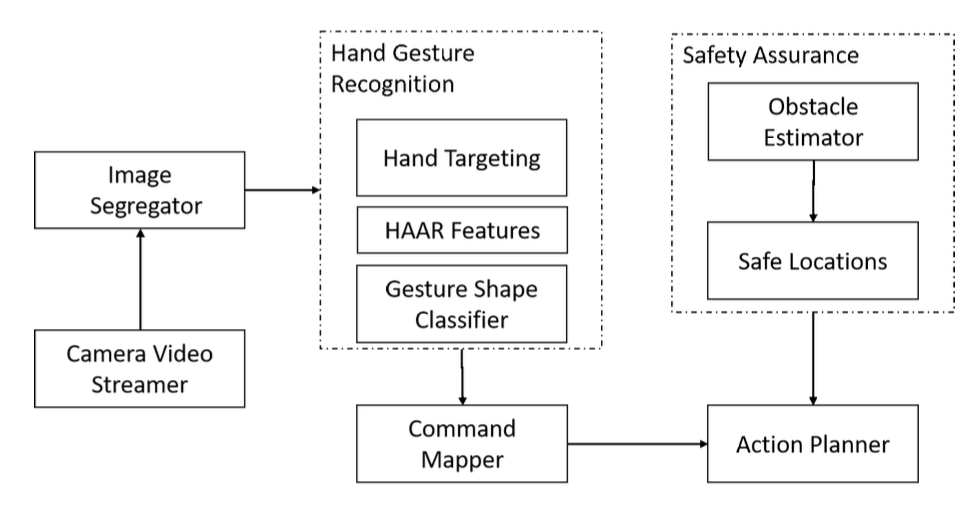
\includegraphics[width=0.8\textwidth]{Haar2.png}
    \caption{چارچوب کنترل پهپاد مبتنی بر ژست}
\end{figure}


\begin{figure}[h]
    \centering
    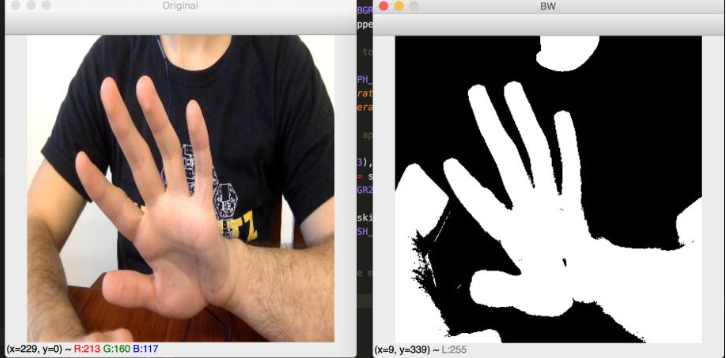
\includegraphics[width=0.5\textwidth]{Haar3.png}
    \caption{ ویژگی های \lr{Haar} برای استفاده از آستانه رنگ پوست برای تشخیص دست}
\end{figure}




\subsubsection{نتیجه بدست آمده}
این پروژه دقت بالایی در تشخیص ژست دست و کنترل پرواز پهپاد دارد. پنج حالت دست مدنظر در این پروژه قرار گرفته‌اند و دقت متوسط آن برابر با ۴۷۱.۹۷ درصد 
است که نشان‌دهنده عملکرد بسیار عالی است. اما لازم به ذکر است که این دقت در پس‌زمینه‌های بهم ریخته و همچنین در شرایط نوری مختلف 
بسیار متغیر است زیرا ویژگی \lr{Haar} به سایه و رنگ‌های درون تصویر بسیار حساس است.



\subsection{مقاله \lr{A real-time hand gesture recognition method}}
در این مقاله در زمینه پردازش تصویر و تشخیص ژست‌های دست، از روش‌های مبتنی بر مدل ظاهری \lr{Appearance Model} به عنوان یک رویکرد موثر استفاده شده‌‌است.
این روش‌ها از ویژگی‌های تصویری و حرکتی دست برای تشخیص و تعیین ژست‌های دست استفاده می‌کنند. در این مقاله، روش تشخیص ژست‌های دست به صورت زمان واقعی و 
قابل اعتماد است که از تشخیص دست، پیگیری دست\LTRfootnote{Hand tracking}، تقسیم‌بندی دست\LTRfootnote{Hand segmentation} و تشخیص ویژگی‌های مقیاس-فضا\LTRfootnote{Scale-space feature detection} برای تشخیص ژست‌های دست استفاده می‌کند.

\subsubsection{روش‌شناسی}
در مقاله از ترکیب متنوعی از روش‌ها و ویژگی‌های تصویری استفاده می‌شود. این ویژگی‌ها به ترتیب به صورت زیر عمل می‌کنند.
\begin{enumerate}
    \item استفاده از روش \lr{Adaboost} برای تشخیص دست، که یک روش معتبر برای تشخیص اشیاء در تصاویر است.
    \item پیگیری دست با استفاده از تشخیص حرکت و رنگ، که از ترکیب تکنیک‌های جریان نوری و نشانه رنگ برای پیگیری دست در تصاویر استفاده می‌شود.
    \item تقسیم‌بندی دست با استفاده از اطلاعات حرکت و رنگ برای تمایز دست از پس‌زمینه و اشیاء دیگر. 
    \item تشخیص ویژگی‌های مقیاس-فضا برای تشخیص ژست‌های دست، که برای شناسایی ساختارهای شبیه به کف دست و انگشتان استفاده می‌شود تا نوع ژست دست توسط ترکیب این ساختارها تعیین شود.
\end{enumerate}
  این روش‌ها و ویژگی‌ها با هم ترکیب شده‌اند تا یک سیستم تشخیص دست پایدار و دقیق برای استفاده در رابط کاربری تعاملی و تشخیص ژست‌های دست در زمینه‌های مختلف ارائه شود.

\begin{figure}[h]
    \centering
    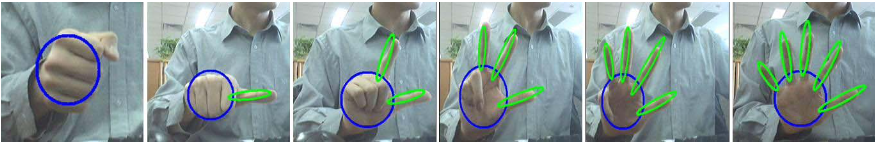
\includegraphics[width=0.8\textwidth]{hand_gesture_feature.png}
    \caption{تشخیص کف دست و انگشتان}
\end{figure}

\subsubsection{نتیجه}
اعمال این روش‌ها نتایج قابل قبولی را به همراه داشته است. دقت مدل در تشخیص ژست‌های دست به صورت میانگین 8.93 درصد بوده و از جمله نتایج مهم آزمایشات می‌توان به تشخیص 
صحیح 2436 فریم از کل 2596 فریم ضبط شده اشاره کرد. این نتایج نشان می‌دهند که روش ارائه شده در این مقاله عملکرد قابل قبولی در تشخیص ژست‌های دست دارد و 
می‌تواند به عنوان یک روش موثر برای تعاملات زمان واقعی استفاده شود.
\cite{fang2007real}


% \subsection{مقاله \lr{Hand Gesture Recognition using Image Processing and Feature Extraction Techniques}}

% \subsubsection{روش‌شناسی}

% \subsubsection{نتیجه}
% \cite{sharma2020hand}



\section{مقالات مربوط به ورودی تصویر دست به مدل}
مقالات این دسته از جمله پرژه‌هایی هستند که بیشتر از آنکه بر روی پیش پردازش کار کنند باید بر روی معماری خود شبکه تمرکز کنند. در این مقالات تمام یا بخشی از تصویر گرفته شده به صورت یک ماتریس از تصویر با پیکسل‌های متعدد به مدل داده می‌شود. تنها موردی که می‌توان در این نوع پروژه‌ها پیش رو گرفت تشخیص موقعیت دست است تا بتوان تنها قسمتی از تصویر را به ورودی شبکه داد که دست در آن وجود دارد تا در حد ممکن انداژه ورودی شبکه و دقت آن افزایش یابد. پس از آن باید توجه داشت معماری شبکه را به گونه‌ای برگزید تا مخصوص پردازش تصویر باشد و بتوان ویژگی‌های تصویر را خود استخراج کند.


\subsection{مقاله \lr{Hand Gestures For Drone Control Using Deep Learning}}
این پروژه با هدف کنترل پهپادها با استفاده از حرکات دستی و با کمک شبکه‌های عمیق یادگیری انجام شده است تا بتوان ۹ حالت مختلف دست را شناسایی و به پهپاد، دستور موردنظر کاربر را داد.


\subsubsection{روش‌شناسی}
در این تحقیق، از معماری شبکه عصبی عمیق \lr{VGG-16} برای تشخیص و تعیین حرکات دستی برای کنترل پهپادها استفاده شده است. شبکه \lr{VGG-16} یکی از معروف‌ترین و پرکاربردترین شبکه‌های عمیق در زمینه بینایی ماشین است که 
شامل 16 لایه عصبی با لایه‌های کانولوشنال و پولینگ می‌باشد. این شبکه برای استخراج ویژگی‌های مهم از تصاویر استفاده می‌شود. ورودی این شبکه تصاویری است که از دوربین متصل به دستگاه اجرایی گرفته می‌شود و سپس این 
تصاویر به شبکه وارد می‌شوند. خروجی این شبکه شامل تشخیص حرکات دستی مانند حرکات مختلف انگشتان و دست‌ها می‌شود که سپس این اطلاعات برای ارسال دستورات کنترلی به پهپاد استفاده می‌شود. این روش نه تنها امکان کنترل دقیق 
و موثر پهپادها را فراهم می‌کند بلکه ارتباط بین انسان و ماشین را نیز بهبود می‌بخشد.

\begin{figure}[h]
    \centering
    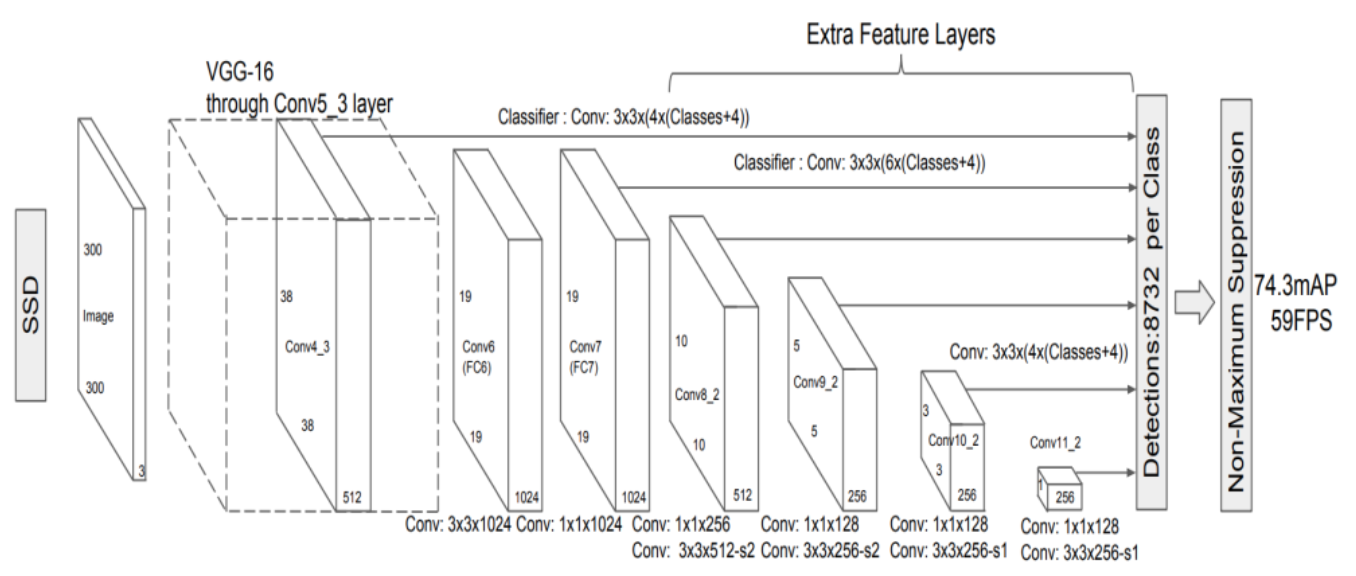
\includegraphics[width=0.8\textwidth]{VGG16.png}
    \caption{معماری \lr{VGG-16}}
\end{figure}

\subsubsection{نتیجه بدست آمده}
 در پروژه این پروژه ۹ حالت دست مدنظر قرار گرفته‌شده و دقت آن برابر ۳.۸۳ درصد است.
 که در بهترین حالت ممکن با پس‌زمینه‌ی مناسب بدست آمده و باید در نظر گرفت که دقت بالایی برای کنترل پهپاد به حساب نمی‌آید.
\cite{hadri2018hand}

\subsection{مقاله \lr{UAV-GESTURE: A Dataset for UAV Control and Gesture Recognition}}
این مقاله به منظور کنترل پهپاد یا خلبان خودکار با استفاده از حرکت دست پیاده‌سازی شده است. به عنوان مثال، حرکت دست از چپ به راست نشان‌دهنده حرکت پهپاد به راست می‌باشد. 
برای اجرای این برنامه، شبکه \lr{P-CNN} طراحی شده است تا بتواند مفهوم تصاویر را تجربه کند.

\subsubsection{روش‌شناسی}
در این مقاله، از شبکه \lr{P-CNN} \LTRfootnote{Pose-based Convolutional Neural Network} برای تشخیص حرکات دست استفاده شده است. این شبکه از اطلاعات حرکت و ظاهر را بر روی مسیرهای بخش‌های بدن انسان (مانند دست راست، 
دست چپ، بدن بالا و بدن کامل) جمع‌آوری می‌کند. این شبکه ابتدا موقعیت دست فرد را با استفاده از جعبه مرزی مشخص می‌کند و سپس تصویر دست با استفاده از فیلترهای مناسب وارد شبکه \lr{P-CNN} می‌شود تا بتواند حرکت دست را پیش‌بینی کند.
\\
در خروجی این مدل، ۱۳ نوع حرکت مختلف وجود دارد که برای پیش‌بینی مفهوم آن‌ها استفاده می‌شود. این حرکات شامل کل دست از شانه تا انگشتان و حرکات آنها می‌شود، که در این پروژه برای دستور دادن به هواپیماهای بزرگ بدون سرنشین در فرودگاه‌ها استفاده می‌شود.
\\
\lr{P-CNN} اطلاعات ظاهر و حرکت را از بخش‌های مختلف بدن استخراج می‌کند و از دو شبکه پیش‌آموزش داده شده برای محاسبه ویژگی‌های \lr{CNN} استفاده می‌کند. برای بخش‌های ظاهر، از شبکه \lr{VGG-f} استفاده می‌شود، در حالی که برای 
بخش‌های حرکتی از شبکه حرکتی از پیاده‌سازی \lr{Action Tube} استفاده می‌شود. ویژگی‌های استاتیک و پویا به طور جداگانه در طول زمان جمع‌آوری می‌شوند تا ویژگی‌های ویدیوی استاتیک و پویا به دست آید.
\\
در نهایت، از روش‌های تجمیع مینیمم و ماکسیمم برای هر بعد از توصیف‌گر بر روی تمام ویدیوها استفاده می‌شود. این روش‌ها برای تشخیص حرکات با دقت بالا استفاده می‌شوند.



\subsubsection{نتیجه}
دارد، اما نیازمندی‌های پیچیده‌ای برای پیاده‌سازی واقعی دارد که از جمله موانعی است که باید در نظر گرفته شود.
در نتیجه، این مقاله یک روش برای کنترل پهپاد با استفاده از حرکت دست پیاده‌سازی کرده است و از شبکه \lr{P-CNN }
برای تشخیص حرکات دست استفاده کرده است. نتایج نشان داده‌اند که این روش با دقت ۹.۹۱ درصد، قابلیت اجرا در پروژه‌های واقعی را دارد، اما نیازمندی‌های پیچیده‌ای برای پیاده‌سازی واقعی دارد که از جمله موانعی است که باید در نظر گرفته شود.
\cite{perera2018uav}




\section{مقالات مربوط به نقاط کلیدی دست}
در این چنین مقالات ورودی شبکه بینایی ماشین برای تشخیص ژست، مختصات نقاط کلیدی دست هستند، که به نوعی یک ویژگی تصویر نیز تلقی می‌شوند. بدین صورت که در ابتدای کار دست کاربرد شناسایی شده و سپس نقاط کلیدی آن استخراج می‌شوند تا بتوان حجم داده ورودی به مدل را تا حد امکان ساده‌تر و در عین حال مفیدتر کرد.

\subsection{مقاله \lr{Hand Gesture Recognition system for Real-Time Application}}
این مقاله به بررسی سیستم تشخیص حرکات دست برای کاربردهای زمان واقعی می‌پردازد. در این سیستم، از الگوریتم \lr{SIFT} برای استخراج ویژگی‌ها از تصاویر
حرکتی استفاده شده و سپس از مدل \lr{Bag of Feature} و رده‌بند \lr{SVM} برای تشخیص دقیق حرکات دست و دستیابی به عملکرد زمان واقعی استفاده شده است.

\subsubsection{روش‌شناسی}
در مقاله اشاره شده، از الگوریتم \lr{SIFT} برای استخراج نقاط کلیدی از تصاویر حرکتی دست استفاده شده است. الگوریتم \lr{SIFT} یک الگوریتم معروف برای استخراج ویژگی‌های برجسته 
و تمایزدهنده از تصاویر است که از مقیاس، جهت و بخشی از تغییرات نوری مستقل برای استخراج این ویژگی‌ها استفاده می‌کند. این ویژگی‌ها به طور قابل توجهی مستقل از 
مقیاس و جهت تصویر هستند و می‌توانند برای تطبیق قابل اعتماد بین دیدگاه‌های مختلف یک شیء یا تصویر استفاده شوند.

\begin{figure}[h]
    \centering
    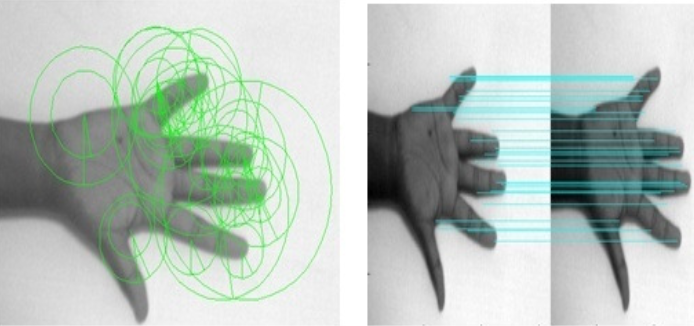
\includegraphics[width=0.5\textwidth]{SIFT.png}
    \caption{تشخیص نقطه کلید و تطبیق توسط \lr{SIFT}}
\end{figure}

\subsubsection{نتیجه}
الگوریتم \lr{SIFT} به عنوان یک ابزار قدرتمند برای استخراج ویژگی‌های برجسته و تمایزدهنده از تصاویر شناخته شده است و در این پروژه با موفقیت برای تشخیص حرکات دست و دستیابی به دقت ۸.۹۰ درصد در تشخیص استفاده شده است.

\cite{murugeswari2014hand}


\subsection{مقاله \lr{An improved hand gesture recognition system using keypoints and hand bounding boxes}}
این مقاله یک سیستم بهبود یافته تشخیص حرکات دست با استفاده از نقاط کلیدی و جعبه‌های محدود کننده دست را معرفی می‌کند تا بتوان نقاط کلیدی دست را پیدا کرد.


\subsubsection{روش‌شناسی}
این پروژه از دو لوله موازی به نام‌های "\lr{MobileNetV2 + FC}" و "\lr{CNN + FC}" تشکیل شده‌است که تصاویر جعبه 
محدود کننده دست و ویژگی‌های استخراج شده از نقاط کلیدی را ترکیب می‌کند و از این طریق ژست دست را پیش‌بینی می‌کند. 
\\
در مدل \lr{MobileNetV2 + FC}، از یک معماری سبک به نام \lr{MobileNetV2} برای استخراج ویژگی‌ها از تصاویر جعبه 
محدود کننده دست استفاده می‌شود. سپس این ویژگی‌ها به یک شبکه عصبی کاملاً متصل (\lr{FC}) داده می‌شوند تا حرکات دست تشخیص داده شوند.
\\
در مدل \lr{CNN + FC} ، در ابتدا نقاط کلیدی دست  که اطلاعات مهمی درباره حرکات دست را شامل می‌شوند پیدا کرده و به یک شبکه عصبی کاملاً متصل (\lr{FC}) وارد می‌شوند تا حرکات دست
تشخیص داده شوند. این مدل از لایه‌های کانولوشنی برای کاهش تعداد پارامترها استفاده می‌کند و سپس از لایه‌های کاملاً متصل برای تشخیص حرکات دست استفاده می‌کند.

\begin{figure}[h]
    \centering
    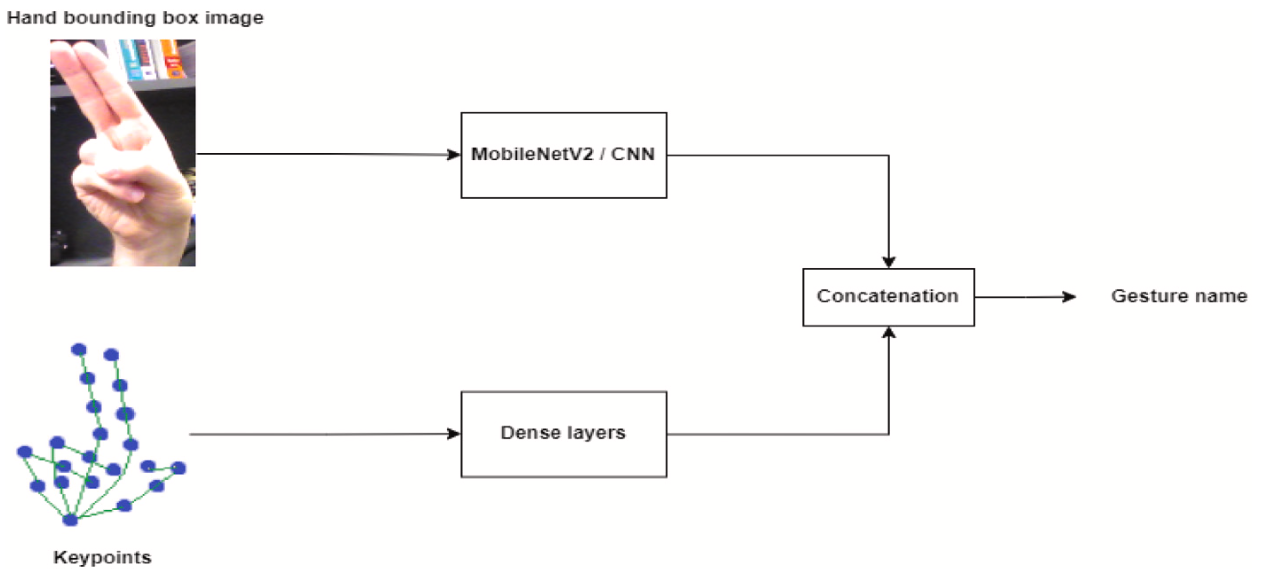
\includegraphics[width=0.8\textwidth]{keypoints_boundingBox.png}
    \caption{معماری ساختار شبکه‌های عصبی دو خط لوله}
\end{figure}


\subsubsection{نتیجه}
در صورتی که دو مدل خروجی‌های متفاوتی را پیش‌بینی کنند، از روش‌های ترکیبی مانند ترکیب احتمالاتی یا استفاده از مدل‌های متفاوت برای شرایط ورودی مختلف استفاده می‌شود تا بهترین تصمیم برای تشخیص ژست دست گرفته شود.
\\
دقت به دست آمده برای تشخیص ۶ ژست دست مختلف در این مقاله در سه دیتاست متفاوت به ترتیب برابر ۹۱، ۹۴ و ۹۶ درصد است.


\cite{dang2022improved}


\subsection{مقاله \lr{Visual gesture recognition based on hand key points}}
این مقاله یک روش تشخیص حرکات ژستی بصری بر اساس نقاط کلید دست ارائه می‌دهد. این روش ابتدا نقاط کلید دست را در تصویر ورودی فعلی تشخیص می‌دهد و سپس حرکات تعریف شده را تشخیص می‌دهد.

\subsubsection{روش‌شناسی}
مدل ارائه شده در این مقاله شامل دو بخش اصلی است: 
\\
مدل تشخیص کف دست که مدل بر اساس ویژگی‌های سخت دست طراحی شده است. برای تشخیص حضور دست در تصویر، از یک مدل \lr{SSD} استفاده شده است که به صورت زمان
واقعی تشخیص انجام می‌دهد. در صورت وجود دست، نتایج توسط یک مستطیل تشخیص می‌شوند.
\\
مدل تشخیص نقاط کلید دست که پس از تشخیص حضور دست در تصویر، از این مدل برای تشخیص 21 مختصات نقطه کلید سه‌بعدی دست استفاده می‌شود.  این مدل از الگوریتم نرمال‌سازی برای محاسبه مختصات افقی و عمودی هر نقطه 
دست استفاده می‌کند. یک سیستم مختصات فضایی برای به دست آوردن مختصات عمق هر نقطه دست نسبت به مبدأ مختصات تعیین شده است. در نهایت، معنای حرکات در تصویر ورودی بر اساس رابطه مکانی بین مختصات نقاط کلید تعیین می‌شود.

\begin{figure}[h]
    \centering
    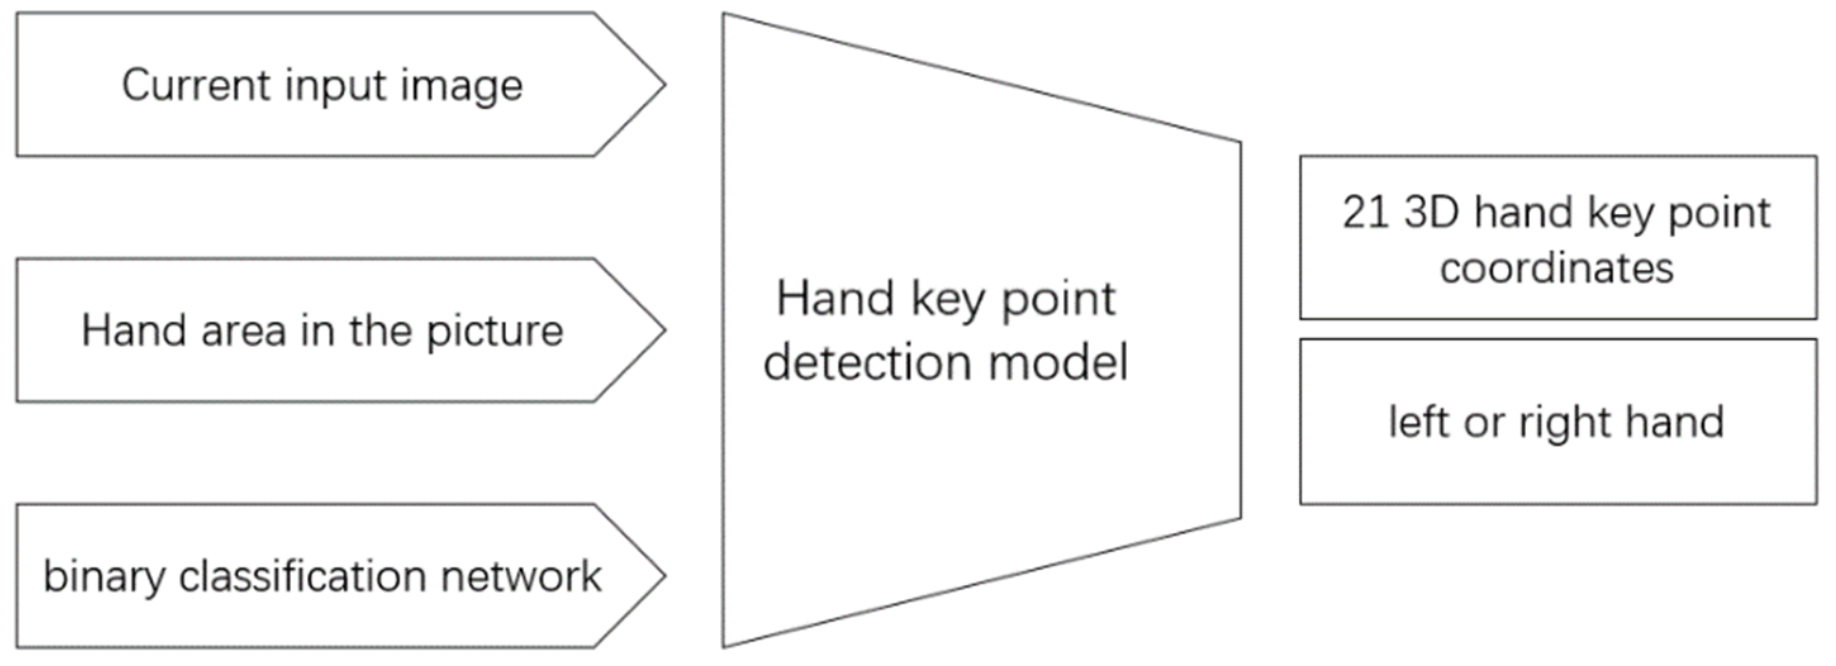
\includegraphics[width=0.8\textwidth]{keypoint.png}
    \caption{ورودی ها و خروجی های مدل تشخیص نقطه کلید دستی}
\end{figure}

\subsubsection{نتیجه}
این روش دارای دقت بالا و عملکرد مناسبی است. دقت متوسط مدل برابر  ۴.۸۵ درصد تا ۵.۹۸ درصد است که با توجه به جزئیات مدل و پیاده‌سازی پیش‌پردازش می‌تواند انعطاف بالایی داشته باشد پس می‌تواند راهکار مناسبی تلقی شود.


\cite{chen2021visual}.


\subsection{مقاله \lr{MediaPipe Hands: On-device Real-time Hand Tracking}}
در این مقاله، از کتابخانه \lr{MediaPipe} برای پیش‌بینی ۲۱ نقطه عطف دست و استفاده در پروژه‌های مختلف از جمله تشخیص ژست دست و افکت‌های \lr{AR} استفاده شده است. ما نیز در پروژه خود از این کتابخانه استفاده می‌کنیم تا یک مدل سبک و ساده پیاده‌سازی کنیم.

\subsubsection{روش‌شناسی}
در این مقاله، از کتابخانه \lr{MediaPipe} برای پیش‌بینی ژست دست استفاده شده است. برای پیاده‌سازی این پروژه، از دو شبکه کانولوشن استفاده شده است. شبکه اول برای پیدا کردن کف دست در تصویر استفاده می‌شود و شبکه دوم ورودی 
موقعیت عکس دست پیدا شده را دریافت و مختصات ۲۱ نقطه عطف را موقعیت‌یابی می‌کند. به کمک این دو شبکه، می‌توان به طور همزمان موقعیت دست‌ها را تشخیص داد و 
نقاط عطف آن‌ها را پیش‌بینی کرد تا برای تشخیص ژست دست در پروژه‌های \lr{AR/VR} و کنترل حرکات دست استفاده شود.

\subsubsection{نتیجه}
مدل‌های طراحی شده در این مقاله برای تشخیص نقاط عطف دست از دقت ۷.۹۵ درصد برخوردار هستند که دقت بسیار بالایی محاسبه می‌شود. این مدل به نور و تصویر پس‌زمینه 
وابسته نیست و دقت متوسط آن در زمینه‌های مختلف اندازه‌گیری شده، لذا مدل را کاربردی و مورد پسندتر می‌کند.

\cite{zhang2020mediapipe} 







\section{مقالات مربوط به اجرای مدل‌های بینایی کامپیوتر روی پهپاد}
\subsection{مقاله \lr{Modeling relation among implementing AI-based drones and sustainable construction project success}}
این مقاله با به بررسی ارتباط بین استفاده از پهپادهای مبتنی بر هوش مصنوعی می‌پردازد. این تحقیق به بررسی تأثیرات مثبتی که ادغام این دو عنصر می‌تواند در بهبود کارایی و پایداری پروژه‌های
ساختمانی داشته باشد، می‌پردازد. از آنجایی که استفاده از پهپادها در صنعت ساختمان به سرعت در حال افزایش است و شرکت‌های ساختمانی تحت فشار روزافزونی برای اتخاذ 
تکنیک‌های بیشتر پایدار و کارآمد قرار دارند، شناخت دقیق‌تری از ارتباط بین موانع و عوامل موفقیت لازم است تا بهترین روش‌ها برای از بین بردن موانع و تضمین موفقیت پهپادها در صنعت مشخص شود.

\subsubsection{روش‌شناسی}
در این تحقیق، از یک مدل معادلات ساختاری هوشمند برای بررسی رابطه بین موانع اجرای پهپادهای مبتنی بر هوش مصنوعی در صنعت ساختمان و موفقیت آنها استفاده شده است.
این مدل شامل یک مجموعه جامع از عوامل موفقیت شامل کیفیت، ایمنی و عوامل محیطی است .
\\
پیاده‌سازی مدل‌ها بر روی پهپادها چالش‌هایی ایجاد می‌کند که باید مورد توجه قرار گیرد. این چالش‌ها شامل موارد زیر می‌شود:
\begin{itemize}
    \item پیچیدگی فنی: پیاده‌سازی مدل‌های هوش مصنوعی بر روی پهپادها نیازمند دانش و تخصص فنی بالا است. این امر نیازمند همکاری بین متخصصان مختلف از حوزه‌های مختلف می‌باشد.
    \item محدودیت‌های سخت‌افزاری: پهپادها ممکن است دارای محدودیت‌های سخت‌افزاری مانند ظرفیت پردازشی و حافظه باشند که ممکن است موانعی برای پیاده‌سازی مدل‌های پیچیده ایجاد کنند.
    \item امنیت و حریم خصوصی: استفاده از هوش مصنوعی در پهپادها نیازمند رعایت استانداردهای امنیتی و حفظ حریم خصوصی است. این امر می‌تواند یک چالش مهم برای پیاده‌سازی مدل‌های هوش مصنوعی باشد.
    \item آموزش و توسعه مدل‌ها: پیاده‌سازی مدل‌های هوش مصنوعی بر روی پهپادها نیازمند آموزش و توسعه مدل‌های مناسب برای محیط و وظایف خاص پهپادها است.
\end{itemize}
این چالش‌ها نشان‌دهنده اهمیت اصلی پیاده‌سازی مدل‌های هوش مصنوعی بر روی پهپادها در صنعت ساختمان است. با غلبه بر این چالش‌ها، می‌توان بهبود 
قابل توجهی در کارایی، ایمنی و پایداری پروژه‌های ساختمانی داشت و از پتانسیل بالقوه این تکنولوژی بهره‌مند شد.
\subsubsection{نتیجه}
این مقاله نه تنها به شناخت بهتر موانع استفاده از پهپادهای مبتنی بر هوش مصنوعی کمک می‌کند، بلکه راهکارهایی برای غلبه بر این موانع و افزایش موفقیت این تکنولوژی در صنعت ساختمان ارائه می‌دهد .از آنجا که
پهپادها می‌توانند به صورت خودکار و هوشمند وظایف مختلفی را انجام دهند، این تکنولوژی می‌تواند به بهبود مدیریت پروژه، کاهش هزینه‌ها و زمان اجرا، افزایش کیفیت و ایمنی کارها کمک کند.
\cite{waqar2023modeling}


\subsection{مقاله \lr{Use of a DJI Tello Drone as an Educational Platform in the Field of Control Engineering}}
این مقاله یک رویکرد نوآورانه را برای استفاده از پهپاد \lr{DJI Tello} به عنوان یک پلتفرم آموزشی در زمینه مهندسی کنترل ارائه می‌دهد. در این مقاله به بررسی نحوه استفاده از ویژگی‌های پهپاد برای 
آموزش مفاهیم کنترل به صورت عملی و جذاب می‌پردازند. همچنین به چگونگی استفاده از پهپاد \lr{DJI Tello} به عنوان یک پلتفرم آموزشی برای آموزش مفاهیم کنترل می‌پردازد.

\subsubsection{روش‌شناسی}
در این مقاله، از پهپاد \lr{DJI Tello} به عنوان یک ابزار آموزشی و تحقیقاتی استفاده شده است. این پهپاد به دلیل داشتن حسگرهای متنوع و امکان برنامه‌نویسی با زبان پایتون، به عنوان یک 
ابزار ایده‌آل و انعطاف‌پذیر برای اهداف آموزشی و تحقیقاتی شناخته می‌شود. مقاله به بررسی ارتباط با پهپاد \lr{DJI Tello} از طریق زبان برنامه‌نویسی پایتون، امکانات 
\lr{SDK} رسمی ارائه شده توسط پهپاد، و نحوه ارتباط با پهپاد از طریق وای‌فای و پورت \lr{UDP} می‌پردازد .
\\
در این مقاله، انتخاب پهپاد \lr{DJI Tello} برای نمایش مفاهیم ابتدایی مربوط به حوزه کنترل به دلایل گوناگونی انجام شده است. از جمله دلایل انتخاب پهپاد می‌توان به محبوبیت رو به افزایش آن در بین عموم مردم،
ویژگی‌های چندگانه آن شامل حسگرها، کنترل بازخورد و الگوریتم‌های تخمین برای انجام وظایف پیچیده، و همچنین قیمت مقرون به صرفه آن نسبت به سایر تجهیزات آموزشی اشاره کرد .
\\
برای پیاده‌سازی مدل‌های هوش مصنوعی بر روی پهپاد \lr{DJI Tello}، از زبان برنامه‌نویسی پایتون و کتابخانه‌های مختلفی که برای ارتباط با حسگرها و سیستم‌های کنترل پروازی پهپاد ارائه شده استفاده می‌شود. این امکانات به دانشجوان این 
امکان را می‌دهد که مدل‌های هوش مصنوعی مختلفی را بر روی پهپاد پیاده‌سازی کرده و عملکرد آن‌ها را تحلیل کنند. به عنوان مثال، کاربران می‌توانند از شبکه‌های عصبی یا منطق فازی برای کنترل حرکت پهپاد استفاده کنند.

\begin{figure}[h]
    \centering
    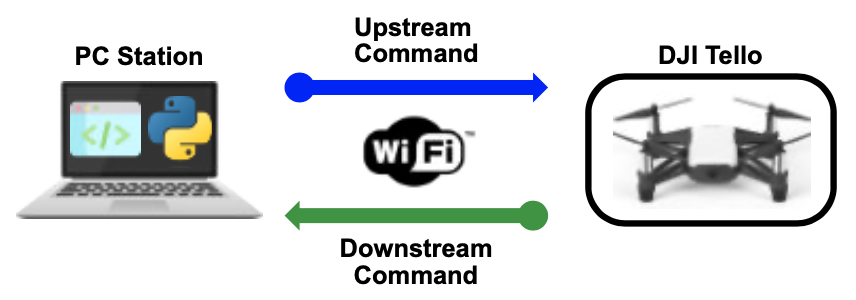
\includegraphics[width=0.8\textwidth]{tello.png}
    \caption{ارتباط با پهپاد \lr{DJI Tello}}
\end{figure}

\subsubsection{نتیجه}
نتیجه این مقاله نشان می‌دهد که استفاده از هوش مصنوعی بر روی پهپاد \lr{DJI Tello} به خوبی عمل می‌کند و این ابزار آموزشی و تحقیقاتی می‌تواند به افراد کمک کند تا مفاهیم پیچیده کنترل و هوش مصنوعی را به صورت عملی و جذاب فرا بگیرند. 
\cite{ghazi2023use}

\section{جمع‌بندی}
در تمام مقالات بررسي شده، پروژه‌ها به گونه‌اي پياده‌سازي شدهاند تا حركات را به طوري كلاسبندي كنند كه در خروجي حتما يكي از ژست‌هاي درنظر گرفته‌شده انتخاب شود. لذا زماني كه دست در حالتي غير از آنها قرار دارد، مدل طراحي شده 
حتما يكي از ژست‌هايي را كه به آن شبيه‌تر است را انتخاب مي‌كند كه اين امر ميتواند براي پياده‌سازي روي پهپاد واقعي مشكل‌زا باشد و حتي هزينه مالي به ارمغان آورد. استخراج ويژگي‌هاي تصوير و يا ورودي خود تصوير به مدل ميتواند بهينه عمل نكند.
% \chapter{روش انجام پروژه}
\section{مقدمه}
برای اجرای این پروژه، روش‌های مختلفی مورد بررسی قرار گرفت تا بتوان بهترین روش را به‌طور موثر  بر روی پهپاد پیاده‌سازی کرد. در نهایت، استفاده از سه شبکه عصبی پیچشی به صورت متوالی به عنوان بهترین راه‌حل انتخاب شد. این سه شبکه به ترتیب وظایف زیر را بر عهده دارند:

\begin{enumerate}
    \item \textbf{آشکارسازی موقعیت کف دست}: هر فریم گرفته‌شده از دوربین پهپاد به ورودی این مدل داده می‌شود. پس از پردازش، خروجی مدل یک جعبه محدودکننده \LTRfootnote{Bounding Box} دست را تولید می‌کند که موقعیت دقیق دست را در تصویر مشخص می‌سازد.
    
    \item \textbf{تشخیص نقاط کلیدی دست}: جعبه مرزی دست که از مدل اول به دست آمده است، به عنوان ورودی به مدل دوم داده می‌شود. این مدل جعبه مرزی را برش زده و ۲۱ نقطه کلیدی سه‌بعدی دست به همراه شاخص دست (راست یا چپ) را تولید می‌کند، که این ویژگی‌ها شامل مفاصل انگشتان و نقاط مهم دست می‌باشند.
    
    \item \textbf{پیش‌بینی علائم دست}: ورودی این مدل، یک ماتریس به ابعاد ۲۱×۲ است که مختصات طول و عرض هر نقطه کلیدی دست را شامل می‌شود. به دلیل محدودیت پهپادها در اندازه‌گیری عمق تصویر و اهمیت کمتر عمق
     در تشخیص علائم مد نظر، فقط مختصات دوبعدی استفاده می‌شود. خروجی این مدل، پیش‌بینی علائم دست کاربر است. این پروژه ۹ علائم گوناگون را مد نظر قرار داده است (کاربر می‌تواند علائم‌ جدیدی اضافه کند). بنابراین، خروجی شبکه پیچشی شامل ۱۰ کلاس است که ۹ کلاس برای علائم مختلف و یک کلاس برای زمانی که هیچ کدام از علائم موجود تشخیص داده نشود، در نظر گرفته شده است.
\end{enumerate}

این سه مدل با همکاری یکدیگر، از تشخیص  مختصات دست تا پیش‌بینی علائم دست را به صورت بهینه و کارآمد انجام می‌دهند، به‌طوری‌که می‌توانند روی پهپادهای موجود پیاده‌سازی شوند و در کاربردهای واقعی مورد استفاده قرار گیرند. بهینه‌سازی‌ها و پیش‌پردازش‌های انجام‌شده در این پروژه،  این اطمینان را حاصل می‌کنند که سیستم با سرعت و دقت بالا عمل کرده و مناسب برای محیط‌های بی‌درنگ باشد.
منبع کد پیاده‌سازی شده برای این پروژه نیز در لینک \href{https://github.com/sara-tajernia/hand-gesture-control_drone}{گیت‌هاب} قابل مشاهده است.

\begin{figure}[h]
    \centering
    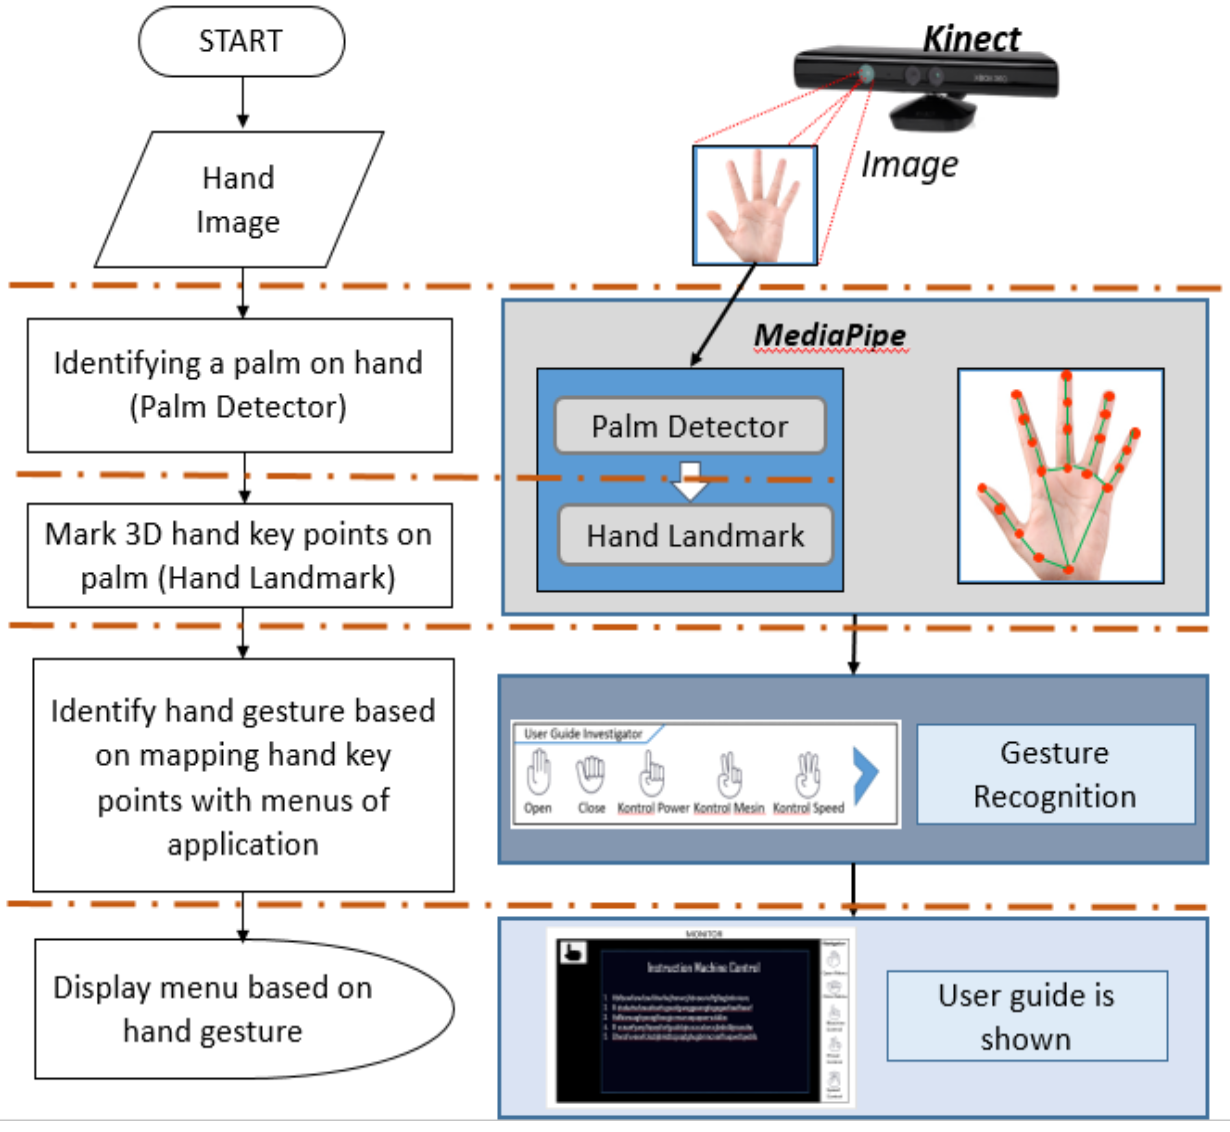
\includegraphics[width=0.8\textwidth]{gesture.png}
    \caption[تشخیص علائم دست با کمک نقاط کلیدی دست]{تشخیص علائم دست با کمک نقاط کلیدی دست \cite{li2012hand}}
\end{figure}

% \section{انتخاب علائم‌های دست متناسب با حرکت پهپاد}
% انتخاب علائم‌های مناسب برای هر یک از حرکات پهپاد از اهمیت ویژه‌ای برخوردار است. چرا که علائم‌هایی که از لحاظ مفهومی به عملکرد پهپاد شبیه هستند راحت‌تر به خاطر سپرده شده و تجربه دلپذیرتری را در کاربر به وجود می‌آورند. 
% ما برای این پروژه 9 علائم دست را در نظر گرفته‌ایم تا بتوان حرکات پایه پهپاد را با آن‌ها انجام داد. این حرکات شامل: حرکت رو به جلو،  حرکت رو به عقب،حرکت به پایین، حرکت به بالا، حرکت به راست، حرکت به چپ، فرود آمدن، 
% ایستادن در موقعیت کنونی و گرفتن عکس است که نمونه علائم دست آن‌ها با توجه به حرکت پهپاد نشان داده شده است.

\section{انتخاب علائم دست مناسب برای کنترل پهپاد}
انتخاب علائم‌ مناسب برای هر یک از حرکات پهپاد از اهمیت ویژه‌ای برخوردار است، زیرا علائم که از لحاظ مفهومی به عملکرد پهپاد شبیه هستند، راحت‌تر به خاطر سپرده می‌شوند و تجربه کاربری دلپذیرتری را ایجاد می‌کنند. برای این پروژه، نه علائم دست در نظر گرفته شده است تا حرکات پایه پهپاد با استفاده از آن‌ها انجام شود. 
این حرکات شامل: حرکت رو به جلو، حرکت رو به عقب، حرکت به سمت پایین، حرکت به سمت بالا،
حرکت به راست، حرکت به چپ، فرود آمدن پهپاد، چرخش ۳۶۰ درجه به صورت ساعتگرد و گرفتن عکس است.
این علائم به گونه‌ای انتخاب شده‌اند که با حرکات پهپاد همخوانی داشته باشند و کاربران بتوانند به راحتی آن‌ها را به خاطر بسپارند و از آن‌ها برای کنترل پهپاد استفاده کنند. نمونه‌های علائم دست متناسب با هر حرکت پهپاد، به طور دقیق در عکس \ref{t} ارائه شده‌اند تا کاربران بتوانند به راحتی از آن‌ها استفاده کنند.

\begin{figure}[h]
    \centering
    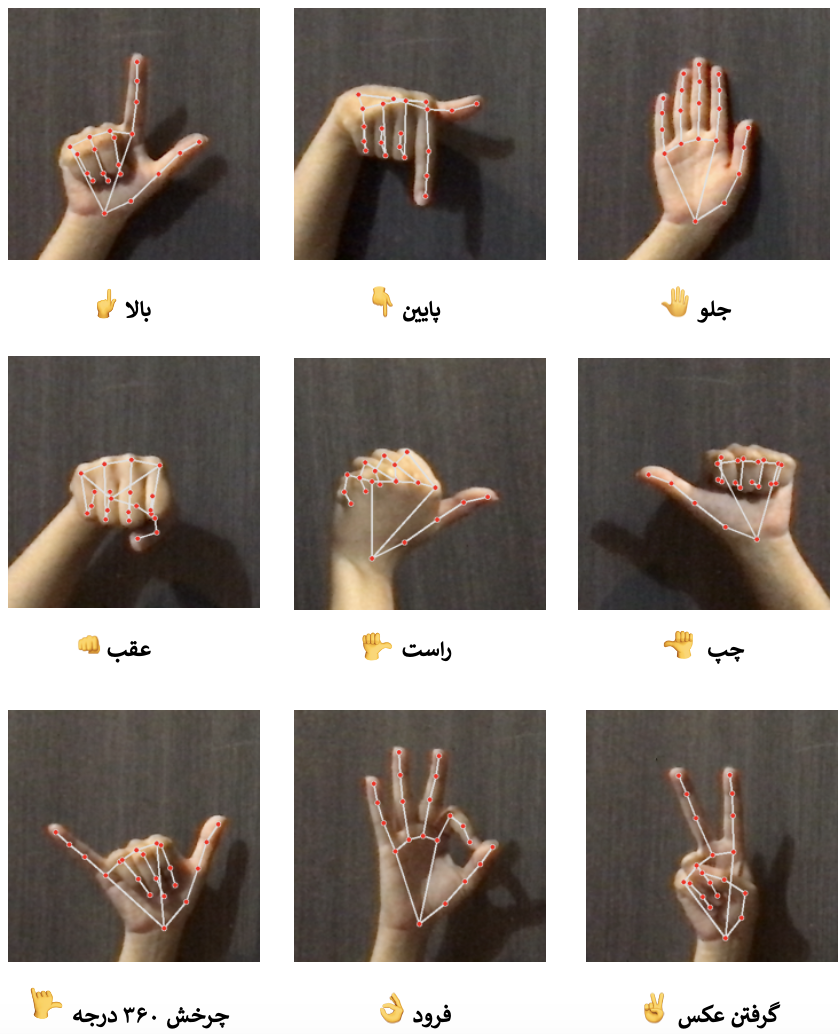
\includegraphics[width=0.7\textwidth]{gestures.png}
    \caption{نمونه‌ای از علائم انتخاب‌شده در مجموعه داده‌ها}
    \label{t}
\end{figure}

\section[مجموع‌داده]{مجموع‌داده \protect\LTRfootnote{Data Set}}
برای جمع‌آوری مجموع‌داده مناسب پروژه، از آنجایی که علائم دست بر اساس عملکرد پهپاد تعیین شده‌اند تا استفاده از آن‌ها برای کاربر مورد پسند باشد، پیدا کردن مجموع‌داده آماده غیرممکن است. جمع‌آوری مجموع‌داده جامع و مناسب از اهمیت
 بالایی برخوردار است زیرا مدل باید به صورت بی‌درنگ کار کند و نمی‌توان از مدل‌های سنگین یادگیری عمیق استفاده کرد. بنابراین، برای افزایش دقت مدل باید از روش‌های دیگری نظیر پیش‌پردازش، پس‌پردازش و استفاده از مجموع‌داده مناسب بهره گرفت.
\\
رویکردهای متفاوتی برای این پروژه پیاده‌سازی شدند تا بهترین راهکار با استفاده از مدلی با حجم کم و در عین حال جامع یافت شود. در نتیجه، مجموع‌داده‌های گوناگونی جمع‌آوری شدند که هر یک از آن‌ها ویژگی خاصی از تصویر
 را به عنوان داده‌ی مورد نیاز جمع‌آوری می‌کردند. این رویکردها شامل استفاده از ورودی کل عکس به صورت پیکسل‌های رنگی، پیدا کردن دست و ذخیره موقعیت آن به صورت پیکسل‌های 256 $\times$ 256 و پیدا کردن نقاط کلیدی دست و ذخیره موقعیت آن‌ها در مجموع‌داده بود. در نهایت، گزینه سوم به عنوان بهترین راه ممکن برای ذخیره داده‌ها و اجرای پروژه انتخاب شد.

برای این پروژه، به منظور امکان اضافه کردن علائم دست جدید توسط کاربر، کدی پیاده‌سازی شد که با باز شدن دوربین و زدن یک حرف  یکسان برای هر کلاس، اطلاعات آن تصویر استخراج شده و در مجموع‌داده ذخیره شود. این روش نه تنها جمع‌آوری داده را راحت‌تر می‌کند، بلکه به کاربر اجازه می‌دهد با زدن یک دکمه، کلاس جدیدی را ایجاد کند.

% \section{کنترل پهپاد}
% اکثر پهپادهای تجاری موجود در بازار یا دارای کنترلرهای ویژه طراحی شده هستند، یا از فرستنده‌های سیگنال اختصاصی و برنامه‌های نرم‌افزاری استفاده می‌کنند که روی
%  دستگاه‌های دستی کاربران مانند تلفن‌های همراه یا تبلت‌ها اجرا می‌شوند. در هر دو حالت، کنترل‌کننده فرمان‌هایی را با اطلاعات دقیق از طریق کانال‌های بی‌سیم مانند وای‌فای یا بلوتوث ارسال می‌کند. 
% \\
% اخیراً محصولاتی تجاری معرفی شده‌اند که از حرکات دست به عنوان یک مکانیسم کنترل قابل اجرا استفاده می‌کنند. برای دریافت علائم، دو رویکرد اصلی وجود دارد:
% \begin{itemize}
%     \item \textbf{استفاده از دستکش‌های ویژه طراحی شده:} کنترل‌کننده بر روی دستکشی که توسط کاربران استفاده می‌شود نصب می‌گردد و در زمان واقعی انحراف، گام و چرخش دست را شناسایی می‌کند تا حرکات مربوط به پهپاد را تشخیص و ارسال کند. از جمله این محصولات می‌توان به \lr{Kd Interactive Aura Drone} و \lr{MenKind Motion Control Drone} اشاره کرد.
%     \item \textbf{استفاده از بینایی ماشین از طریق دوربین:}   این دستگاه‌ها از دوربین نصب شده روی پهپاد استفاده می‌کنند تا بتوانند در لحظه تشخیص دهند که دست کاربر کجاست و در چه حالتی قرار دارد تا پهپاد را کنترل کنند. از جمله این محصولات می‌توان به پهپاد دی‌جی‌آی اسپارک \LTRfootnote{DJI Spark Drone} اشاره کرد.
% \end{itemize}


\section{ابزار‌ها و نرم افزار های مورد استفاده}
برای پیاده‌سازی این پروژه از ابزار‌ها، نرم‌افزار‌ها و کتاب‌خانه‌های گوناگونی استفاده شده‌است که در ادامه به توضیح دقیق آن‌ها می‌پردازیم. قابل ذکر است که از کتاب‌خانه‌هایی از جمله سی‌اس‌وی \LTRfootnote{Csv}،کپی \LTRfootnote{Copy}، ایترتولز\LTRfootnote{Itertools} و اواس\LTRfootnote{Os} نیز در قسمت‌هایی از پروژه به‌کار برده‌شده است که به دلیل استفاده جزئی توضیح داده نشده‌اند.

% \subsection{زبان برنامه‌نویسی پایتون}

\subsection[کتاب‌خانه تنسورفلو]{کتاب‌خانه تنسورفلو ‌\protect\LTRfootnote{TensorFlow}}
تنسورفلو یک کتاب‌خانه نرم‌افزاری رایگان و منبع باز برای یادگیری ماشین و هوش مصنوعی است. این کتاب‌خانه توسط گوگل برین توسعه داده‌شده و می‌تواند در طیف وسیعی 
از وظایف یادگیری ماشین مورد استفاده قرار گیرد. همچنین تمرکز ویژه‌ای بر آموزش و استنتاج شبکه‌های عصبی عمیق دارد. 
\\
تنسورفلو انعطاف‌پذیری بالایی دارد که می‌تواند برای انواع مختلف مدل‌های یادگیری ماشین از جمله شبکه‌های عصبی پیچشی، شبکه‌های عصبی بازگشتی و شبکه‌های مولد متخاصم\LTRfootnote{Generative Adversarial Network} مورد استفاده قرار گیرد.
تنسورفلو قابلیت اجرای مدل‌ها بر روی پردازنده‌های چندگانه، پردازنده‌های گرافیکی\LTRfootnote{Graphics Processing Unit} و واحد پردازشی تنسو\LTRfootnote{Tensor Processing Unit} را دارد. همچنین به دلیل محبوبیت و پشتیبانی گسترده،
منابع آموزشی و کتاب‌خانه‌های جانبی فراوانی برای آن وجود دارد. به طور کلی،تنسورفلو یکی از ابزارهای قدرتمند و پرکاربرد در حوزه یادگیری ماشین و هوش مصنوعی است \cite{Introduc60:online}.


\subsection[کتاب‌خانه سایکیت لرن]{کتاب‌خانه سایکیت لرن\protect\LTRfootnote{Scikit-learn}}
سایکیت لرن که با نام‌های \lr{Scikits.learn} و \lr{Sklearn} نیز شناخته می‌شود یک کتاب‌خانه یادگیری ماشین رایگان و منبع باز برای زبان برنامه‌نویسی پایتون است. این کتاب‌خانه شامل الگوریتم‌های مختلفی برای طبقه‌بندی،
رگرسیون و خوشه‌بندی مانند ماشین‌های بردار پشتیبان، جنگل‌های تصادفی
\LTRfootnote{Random Forest}
، تقویت گرادیان
\LTRfootnote{Gradian activation}
،میانگین-کی \LTRfootnote{K-means} و دی‌بی اسکن\LTRfootnote{DBSCAN} می‌باشد. سایکیت لرن به طور ویژه برای تعامل با
کتاب‌خانه‌های  نام‌پای\LTRfootnote{NumPy} و سای‌پای\LTRfootnote{SciPy} طراحی شده است و ابزارهای متنوعی برای پیش‌پردازش داده‌ها، انتخاب و ارزیابی مدل‌ها و کاهش بعد فراهم می‌کند. این کتاب‌خانه به کاربران کمک می‌کند تا به راحتی از آن در پروژه‌های 
یادگیری ماشین استفاده کنند. این کتاب‌خانه به دلیل سادگی و کارایی خود در بین محققان و مهندسان داده بسیار محبوب است و امکانات وسیعی را برای توسعه و ارزیابی مدل‌های یادگیری ماشین فراهم می‌کند \cite{scikitle22:online}.

\subsection[رابط برنامه‌نویسی کراس]{رابط برنامه‌نویسی کراس\protect\LTRfootnote{Keras}}
کراس یک رابط برنامه‌نویسی\LTRfootnote{Application Programming Interface} یادگیری عمیق است که به زبان پایتون نوشته شده و می‌تواند بر روی  تنسورفلو و پای‌تورچ \LTRfootnote{PyTorch} اجرا شود. هدف اصلی کراس کاهش پیچیدگی‌ها و بار شناختی توسعه‌دهندگان است، 
به طوری که آن‌ها بتوانند روی بخش‌های حیاتی و مهم پروژه‌های یادگیری ماشین تمرکز کنند. این رابط برنامه‌نویسی با رابط کاربری ساده و کاربرپسند، امکان توسعه سریع مدل‌های پیچیده را فراهم
می‌کند. کراس عملکرد بالایی دارد و توسط سازمان‌های بزرگی نظیر ناسا، یوتیوب و \lr{Waymo} برای تحلیل داده‌ها، بهبود الگوریتم‌های توصیه‌گر و توسعه سیستم‌های خودران مورد استفاده قرار 
می‌گیرد. این کتاب‌خانه با مستندات جامع و پشتیبانی از جامعه کاربری بزرگ، به یکی از ابزارهای محبوب در حوزه یادگیری عمیق تبدیل شده‌است \cite{AboutKer57:online}.

% \subsection{کتاب‌خانه‌های\lr{MediaPipe}}
% \lr{MediaPipe} مجموعه ای از کتاب‌خانه ها و ابزارهایی است که از تکنیک‌های هوش مصنوعی و یادگیری ماشین در برنامه‌های خود استفاده می‌کند.
% این کتاب‌خانه برای برنامه‌نویسان یادگیری ماشین از جمله محققان، دانشجویان و توسعه‌دهندگان نرم‌افزار، که برنامه‌های کاربردی یادگیری ماشین را پیاده‌سازی می‌کنند، نمونه‌های
% اولیه فناوری را طراحی می‌کند تا بتوان پروژه‌ها را تا حد امکان ساده کرد.
% برنامه‌هایی که داده‌های حسی مثل ویدیو و صدا را با نرخ فریم بالا پردازش می‌کند تا تجربه کاربر را بهتر کند. مراحل پردازش یا مدل‌های استنتاجی ممکن است دشوار باشد، چون 
% گاهی اتصال بین مراحل زیاد است. همچنین، توسعه برنامه برای پلتفرم‌ زمان‌بر است \cite{lugaresi2019mediapipe}. 
% \\
% \lr{Media Pipe} این چالش‌ها را با انتزاع و اتصال مدل‌های مختلف به یکدیگر در یک چارچوب مناسب حل می‌کند. با استفاده از \lr{MediaPipe}، می‌توان یک لوله پردازش را به صورت 
% گراف از اجزای مختلف، از جمله مدل‌های استنتاجی و عملکردهای پردازش رسانه‌ای، ساخت.
% همچنین این کتاب‌خانه می‌تواند مطابق با نیازهای افراد خود سفارشی شود و در پلتفرم‌های مختلف توسعه پیدا کند.
% \\
% در مجموعه \lr{MediaPipe} نیز از کتاب‌خانه‌های مختلفی برای پیاده‌سازی برنامه ها استفاده می‌شود. از جمله آن‌ها می‌توان به \lr{TensorFlow}، \lr{PyTorch}، اپن سی‌وی، \lr{CNTK} و \lr{MXNet} اشاره کرد \cite{harris2021applying}. 

\subsection{کتاب‌خانه‌های دی‌جی‌آی تلوپی\protect\LTRfootnote{Djitellopy}}
کتاب‌خانه دی‌جی‌آی تلوپی یکی از کتاب‌خانه‌های محبوب برای کنترل پهپاد دی‌جی‌آی تلو با استفاده از زبان برنامه‌نویسی پایتون است. این کتاب‌خانه امکانات پیشرفته‌ای را به کاربران می‌دهد تا با استفاده 
از دستورات پیش‌فرض مختلف به راحتی حرکات پهپاد را کنترل کند. دی‌جی‌آی تلوپی شامل توابع بسیاری است که کاربران را قادر می‌سازد تا به سادگی حرکات پهپاد را کنترل کنند.
\\
علاوه بر این، این کتاب‌خانه شامل برنامه‌هایی است که از کنترل حرکات پهپاد با استفاده از کلیدهای صفحه کلید و یا استفاده از دوربین پهپاد برای ایجاد پانوراما، پشتیبانی می‌کند. از آنجایی که کتاب‌خانه دی‌جی‌آی تلوپی امکانات پیشرفته‌ای برای کنترل پهپاد دی‌جی‌آی تلو فراهم می‌کند، این کتاب‌خانه 
می‌تواند یک ابزار قدرتمند برای توسعه و کنترل پروژه‌های مربوط به پهپاد باشد و به کاربران امکان کنترل دقیق و انعطاف‌پذیری را برای انجام وظایف مختلف فراهم کند.
\\
همچنین این کتاب‌خانه توانایی  کنترل دسته ای از پهپادها به غیر از دی‌جی‌آی تلو را دارد و دارای تمام  دستورالعمل‌هایی است که پهپاد دی‌جی‌آی تلو توانایی انجام آنها را دارد.


\subsection[کتاب‌خانه‌های مدیاپایپ]{کتاب‌خانه‌های مدیاپایپ \protect\LTRfootnote{MediaPipe}}
مدیاپایپ مجموعه‌ای از کتاب‌خانه‌ها و ابزارهایی است که از تکنیک‌های هوش مصنوعی و یادگیری ماشین در برنامه‌های خود استفاده می‌کند. این کتاب‌خانه برای برنامه‌نویسان یادگیری ماشین از جمله محققان، دانشجویان و توسعه‌دهندگان
 نرم‌افزار، که برنامه‌های کاربردی یادگیری ماشین را پیاده‌سازی می‌کنند، نمونه‌های اولیه و از پیش آموزش دیده‌ای را طراحی می‌کند تا پروژه‌ها را تا حد امکان ساده کند.
\\
برنامه‌هایی که داده‌های حسی مانند ویدیو و صدا را با نرخ فریم بالا پردازش می‌کنند و به‌طور خاص برای بهبود تجربه کاربر
 طراحی شده‌اند چالش‌های مختلفی دارند. برای مثال مراحل پردازش یا مدل‌های استنتاجی ممکن است پیچیده باشند، زیرا گاهی اتصال بین مراحل بسیار زیاد است. همچنین، توسعه برنامه برای پلتفرم‌های مختلف نیز می‌تواند زمان‌بر باشد \cite{lugaresi2019mediapipe}. 
\\
مدیاپایپ این چالش‌ها را با انتزاع و اتصال مدل‌های مختلف به یکدیگر در یک چارچوب مناسب حل می‌کند. با استفاده از مدیاپایپ، می‌توان یک لوله‌ی پردازش را به صورت گراف از اجزای مختلف، از جمله مدل‌های استنتاجی و عملکردهای پردازش رسانه‌ای، ساخت. این کتاب‌خانه همچنین قابل سفارشی‌سازی است و می‌تواند بر روی پلتفرم‌های مختلف توسعه یابد.
\\
در مجموعه مدیاپایپ نیز از کتاب‌خانه‌های مختلفی برای پیاده‌سازی برنامه‌ها استفاده می‌شود. از جمله آن‌ها می‌توان به تنسورفلو، پای‌تورچ، اپن سی‌پی
\LTRfootnote{OpenCv}
، \lr{CNTK} و \lr{MXNet} اشاره کرد \cite{harris2021applying}.


\begin{figure}[h]
    \centering
    \includegraphics[width=0.85\textwidth]{mediapipe2.png}
    \caption[برخی کاربردهای کتاب‌خانه مدیاپایپ]{برخی کاربردهای کتاب‌خانه مدیاپایپ \cite{harris2021applying}}
\end{figure}

\subsection{کتاب‌خانه نام‌پای}
نام‌پای کتاب‌خانه‌ای برای محاسبات علمی در پایتون است که آرایه‌های چندبعدی و توابعی برای عملیات سریع  بر روی این آرایه‌ها ارائه می‌دهد. در هسته‌ی نام‌پای، شیء \lr{Ndarray} وجود 
دارد که آرایه‌های \lr{n}-بعدی تشکیل شده از داده‌های همگن را در بر می‌گیرد و بسیاری از عملیات‌های ریاضی بر روی آن‌ها انجام می‌شود. این کتاب‌خانه امکان انجام عملیات ریاضی پیشرفته و سایر 
عملیات‌ها روی تعداد زیادی داده را با کارایی بالا فراهم می‌کند، که نسبت به استفاده از توابع از پیش تعریف شده زبان برنامه‌نویسی پایتون کارآمدی و حجم کد کمتری دارد \cite{WhatisNu62:online}.

\subsection[کتاب‌خانه مت‌پلات لیب]{کتاب‌خانه مت‌پلات لیپ \LTRfootnote{Matplotlib}}
مت‌پلات لیپ یک کتاب‌خانه چند پلتفرمی\LTRfootnote{Cross-Platform}، برای تجسم داده‌ها و نمودارهای گرافیکی از جمله هیستوگرام، نمودارهای پراکنده و نمودار میله‌ای برای زبان برنامه‌نویسی
پایتون است. توسعه دهندگان همچنین می توانند از رابط‌های برنامه‌نویسی مت‌پلات لیپ برای جاسازی نمودارها در برنامه‌های دارای رابط کاربری گرافیکی نیز استفاده کنند.
\\
یک آغازگر
\LTRfootnote{Script}
مت‌پلات لیپ  درون زبان برنامه‌نویسی پایتون به گونه‌ای ساختار یافته است که چند خط کد تنها چیزی است که در بیشتر موارد برای تولید نمودار داده بصری مورد نیاز است. مت‌پلات لیپ دو رابط برنامه‌نویسی را پوشش می دهد:
\\
رابط برنامه‌نویسی پای‌پلات \LTRfootnote{Pyplot}، که سلسله مراتبی از اشیاء درون کد پایتون است که در بالای آن \lr{Matplotlib.Pyplot} قرار دارد. و رابط برنامه‌نویسی اشیاء گرا\LTRfootnote{Object Oriented} که می تواند 
با انعطاف پذیری بیشتری نسبت به \lr{Pyplot} سرهم شوند. این رابط برنامه‌نویسی دسترسی مستقیم به لایه‌های پشتی مت‌پلات لیب
\LTRfootnote{Matplotlib Backend}
را فراهم می کند \cite{Introduc75:online}.

\subsection{کتاب‌خانه اپن سی‌وی}
اپن سی‌وی یک کتاب‌خانه متن باز برای بینایی ماشین و یادگیری ماشین است که برای فراهم کردن زیرساخت مشترک برای برنامه‌های بینایی ماشین و تسریع استفاده از ادراک ماشین در محصولات
تجاری طراحی شده است. این کتاب‌خانه شامل بیش از 2500 الگوریتم بهینه‌سازی شده است که مجموعه جامعی از الگوریتم‌های کلاسیک و جدید بینایی ماشین و یادگیری ماشین 
را فراهم می‌کند. اپن سی‌وی به طور گسترده‌ای در شرکت‌ها، گروه‌های تحقیقاتی و نهادهای دولتی برای انجام پروژه‌های بینایی ماشین و یادگیری ماشین استفاده می‌شود. این کتاب‌خانه رابط‌های برنامه‌نویسی 
متعددی از جمله 
سی پلاس پلاس، پایتون ،جاوا و متلب را دارد که امکان انجام پروژه‌های بینایی ماشین با استفاده از زبان‌های برنامه‌نویسی مختلف را فراهم می‌کند \cite{AboutOpe4:online}.

\subsection{پهپاد دی‌جی‌آی تلو}
پهپاد دی‌جی‌آی تلو یک پهپاد کوادکوپتر کوچک و قابل برنامه‌ریزی است که برای مصارف آموزشی و تست پروتوتایپ توسط شرکت دی‌جی‌آی طراحی شده است. این پهپاد دارای ویژگی‌های ویژه‌ای مانند حرکات پایه‌ای کوادکوپتری و همچنین تکنولوژی 
کنترل پرواز دی‌جی‌آی و یک پردازنده بسیار قوی از شرکت اینتل است. دوربین 5 مگاپیکسلی این پهپاد امکان ضبط ویدیو با کیفیت مناسب را فراهم می‌کند. همچنین، پهپاد دارای یک سیستم موقعیت‌یابی بصری\LTRfootnote{Vision Positioning System} است که شامل 
یک دوربین و یک ماژول مادون قرمز 3 بعدی است و قادر است در فواصل سه تا سی متر ارتفاع  را کار کند .
\\
هسته پهپاد به عنوان مرکز پردازشی و کنترلی آن عمل می‌کند و از یک پردازنده اینتل قدرتمند پشتیبانی می‌کند. پهپاد دی‌جی‌آی تلو برای اجرای پروژه‌های هوش مصنوعی مانند تشخیص اشیاء روی پهپاد، از زبان 
برنامه‌نویسی پایتون و بسته توسعه نرم‌افزار مربوطه پشتیبانی می‌کند. این بسته توسعه نرم‌افزار به کاربران این امکان را می‌دهد که نمونه‌های اولیه پروژه‌های خود را توسعه دهند و آن‌ها را بر روی پهپاد اجرا کنند .
\\
این پهپاد دارای یک باتری با ویژگی‌های خاصی مانند زمان پرواز زیاد و زمان شارژ کم است که می‌تواند از نظر عملکرد و ماندگاری باتری نسبت به پهپاد‌های دیگر مزیت داشته باشد. همچنین، پروژه‌های هوش مصنوعی که روی پهپاد دی‌جی‌آی تلو پیاده‌سازی می‌شوند، 
می‌توانند شامل تشخیص اشیاء، پیش‌بینی حرکت‌ها و یا حتی خودکارسازی فرآیندهای پروازی باشند. از جمله مدل‌های هوش مصنوعی که می‌تواند روی پهپاد دی‌جی‌آی تلو پیاده‌سازی شود، می‌توان به یولو سه \LTRfootnote{YOLOv3} اشاره کرد که برای تشخیص اشیاء با دقت بالا استفاده می‌شود \cite{bhujbal2022custom}.

\begin{figure}[h]
    \centering
    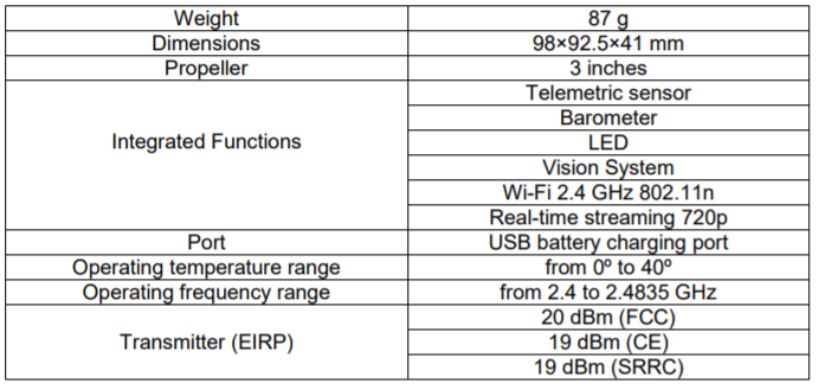
\includegraphics[width=0.7\textwidth]{table.png}
    \caption[طلاعات پهپاد دی‌جی‌آی تلو]{اطلاعات پهپاد دی‌جی‌آی تلو \cite{bhujbal2022custom}}
\end{figure}


\section{روند اجرای پروژه}
در این پروژه از ۳ مدل اصلی به صورت متوالی برای پیش‌بینی تعیین علائم دست استفاده شده‌ است. این سه مدل شامل تشخیص مرز‌های دست، تشخیص نقاط کلیدی دست و در نهایت تعیین علائم دست است. پس از استفاده از این مدل‌های بینایی ماشین، دستور پیش‌بینی شده برای اجرا به پهپاد دی‌جی‌آی تلو فرستاده می‌شود.
\\
برای بهینه کردن روند این پروژه ماژول‌های گوناگونی از جمله محدود كننده جريان بی‌درنگ، تشخيص با استفاده از مستطيل محدودکننده، برش تصوير،  ورود نقاط عطف به مستطيل محدودکننده و ارائه كننده حاشيه نويسي نیز پیاده‌سازی شده‌اند تا روند پیش‌بینی علائم دست را با سرعت و دقت بالاتری اجرا کنند.

\begin{figure}[h]
    \centering
    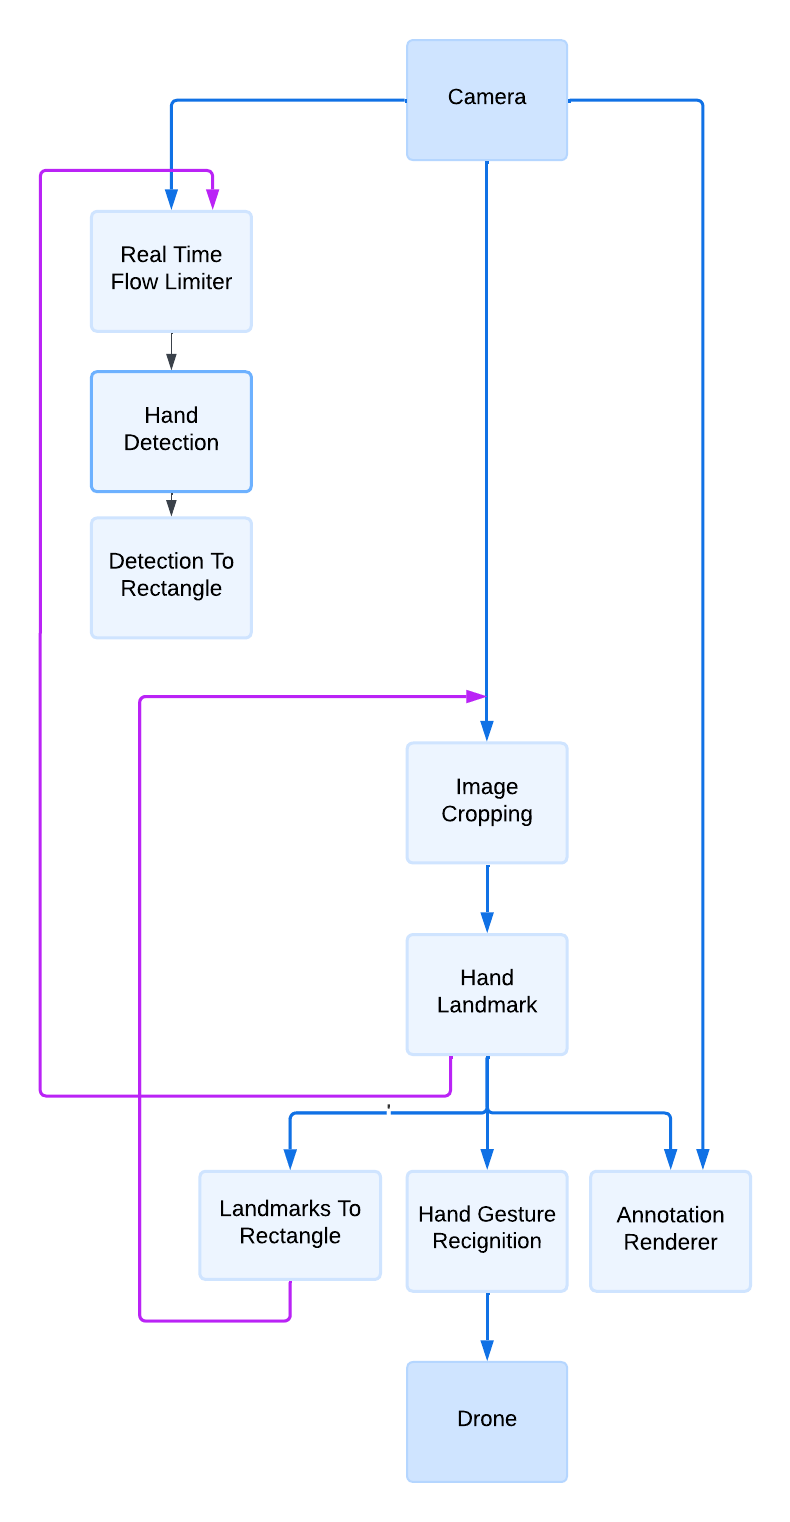
\includegraphics[width=0.8\textwidth]{flowchart.png}
    \caption{روندنمای پروژه}
\end{figure}



% \section{مدیاپایپ}
% برای پیاده سازی شبکه‌های تشخیص کف دست و پیدا کردن نقاط عطف دست از مدل‌های از قبل آموزش دیده\LTRfootnote{Pretrained} کتاب‌خانه مدیاپایپ کمک گرفته‌شده است. مدیاپایپ  از یک خط لوله
% یادگیری ماشین متشکل از چندین مدل که با هم کار می‌کنند استفاده می‌کند: یک مدل تشخیص کف دست \LTRfootnote{Palm Detection Model}
% که تصویر را از ورودی می‌گیرد و  عکس محدوده دست را به عنوان خروجی دریافت می‌کند و یک مدل تشخیص نقاط عطف دست \LTRfootnote{Hand Landmark Model}
% که عکس دست را به عنوان ورودی گرفته و مختصات‌ 21 نقطه کلیدی بند‌های انگشتان دست را در ناحیه دست تشخیص می‌دهد.
% در عکس \ref{Chart} ماژول‌های مربوط به شناسایی نقاط کلیدی نشان داده‌شده که به تفکیک هر کدام را توضیح خواهیم داد.

% \begin{figure}[h]
%     \centering
%     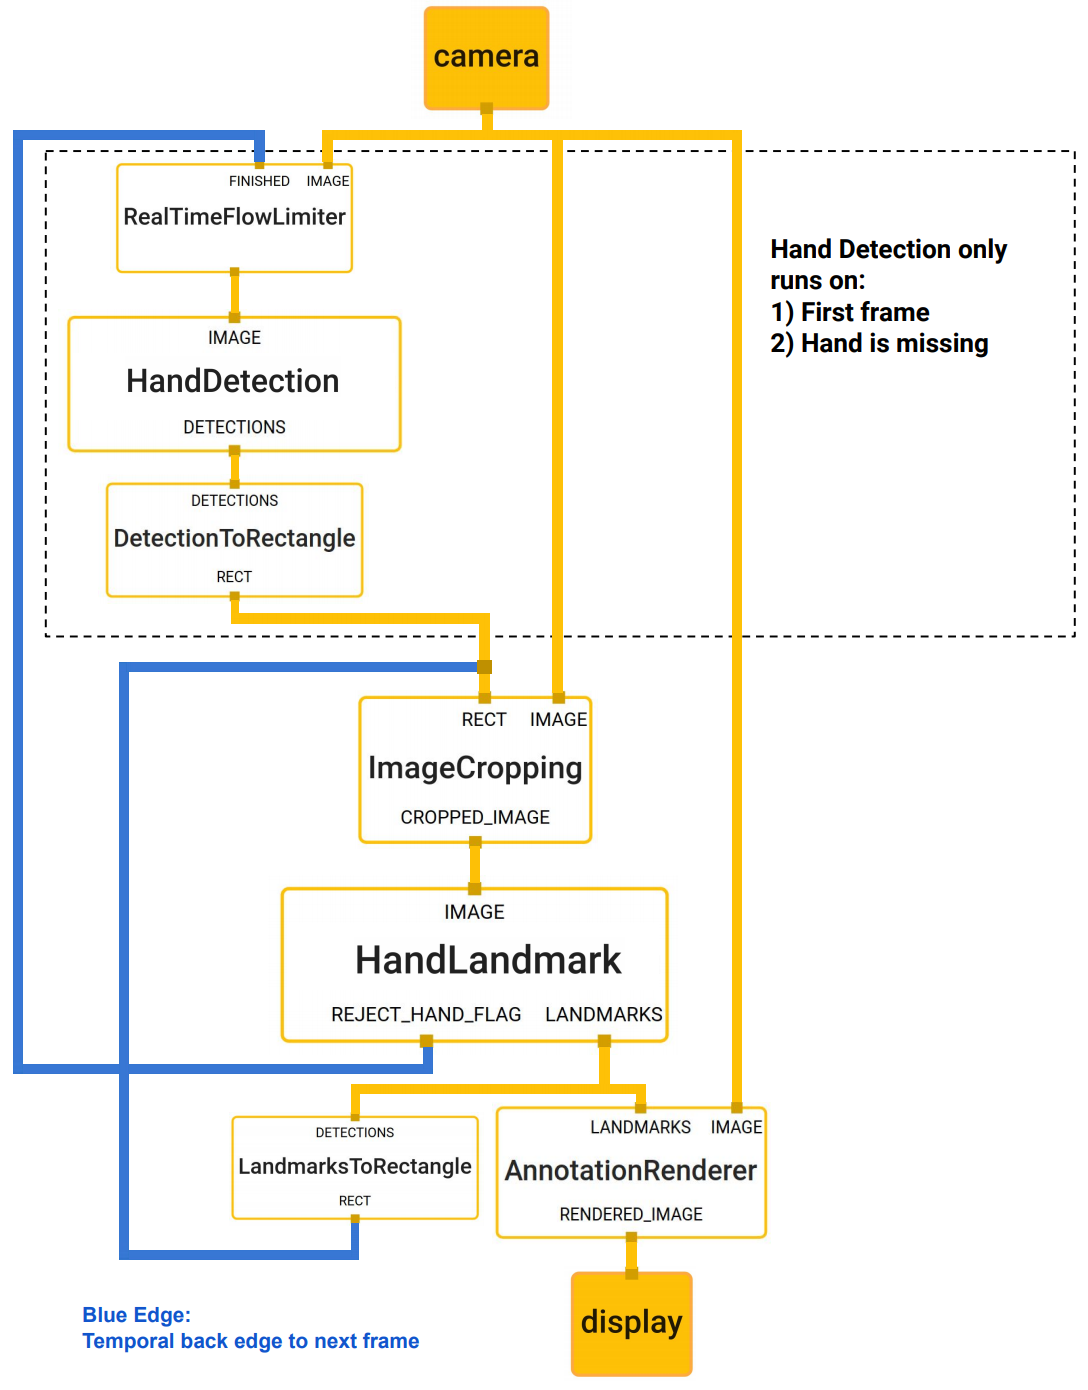
\includegraphics[width=0.7\textwidth]{hand_chart.png}
%     \caption{نمودار \lr{MediaPipe} برای شناسایی نقاط کلیدی دست}
%     \label{chart}
% \end{figure}



\section{تشخیص دست\protect\LTRfootnote{Hand Detection}}
\subsection{مدل تشخیص کف دست}
ماژول تشخیص کف دست، یکی از سه ماژول اصلی است که با دقت متوسط ۷.۹۵ درصد عمل می‌کند. این دقت بالا با استفاده از استراتژی‌های مختلف به دست آمده است. این ماژول به جای تشخیص دست، 
از یک مدل تشخیص کف دست استفاده می‌کند زیرا تشخیص محدوده‌های اجسام سفت و سخت مانند کف دست و مشت بسیار ساده‌تر از تشخیص دست‌ها با انگشتان مفصلی است. در این ماژول از
 الگوریتم سرکوب غیر حداکثری برای حذف تشخیص‌های تکراری و انتخاب مرتبط‌ترین اشیاء شناسایی شده استفاده می‌شود که به کاهش نتیجه‌های مثبت کاذب و پیچیدگی محاسباتی کمک می‌کند و وظیفه اصلی آن تشخیص دست در تصویر و محاسبه مکان دقیق دست است.

این ماژول قادر است به‌صورت دقیق و کارآمد موقعیت دست‌ها را شناسایی کند و نواحی مربوطه را برای
 پردازش‌های بعدی فراهم کند. ورودی این ماژول شامل تصویر یا فریم ویدیو است، در حالی که خروجی آن شامل مستطیل‌های محدوده دست‌ها، نمرات اطمینان و در صورت فعال بودن، دست غالب\LTRfootnote{Handedness} است. معماری این ماژول شامل 
 مراحل پیش پردازش\LTRfootnote{Preprocessing}،مدل تشخیص دست و پس پردازش\LTRfootnote{Postprocessing} است که به ترتیب شامل نرمال‌سازی و تغییر اندازه تصویر، شبکه عصبی تشخیص دست و فیلترینگ و محاسبه نواحی مستطیلی دست‌ها می‌باشد.

وظیفه اصلی ماژول شناسایی و محصور کردن دست‌ها در تصاویر و ویدیوها است که در کاربردهای مختلفی از جمله تشخیص حرکات دست، رابط‌های کاربری بدون لمس، تحلیل رفتار و علائم و کمک به افراد کم‌توان
 از اهمیت برخوردار است. این ماژول به توسعه‌دهندگان این امکان را می‌دهد که به راحتی و با دقت بالا دست‌ها را در تصاویر و ویدیوها شناسایی کرده و از این اطلاعات برای پردازش‌های بعدی استفاده کنند.


\begin{figure}[h]
    \centering
    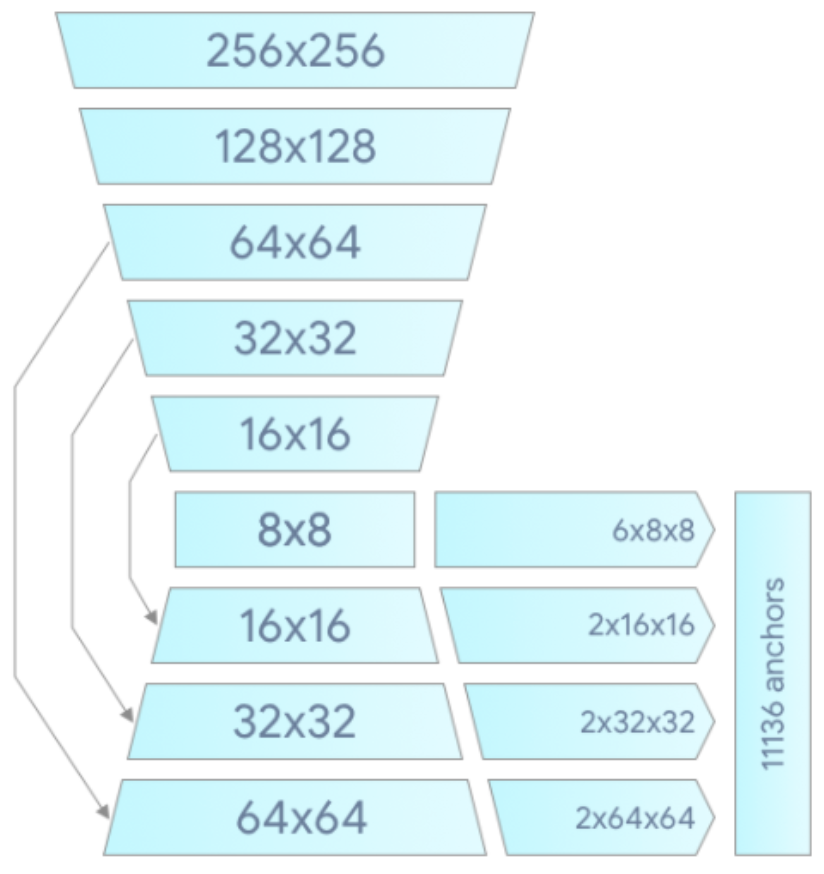
\includegraphics[width=0.4\textwidth]{hand_detector.png}
    \caption[معماری مدل آشکارساز کف دست]{معماری مدل آشکارساز کف دست\cite{zhang2020mediapipe}}
\end{figure}

\subsection{محدود کننده جریان بی‌درنگ\protect\LTRfootnote{Real Time Flow Limiter}}
ماژول محدود کننده جریان بی‌درنگ وظیفه‌ی محدود کردن پردازش برای رسیدن برنامه به سرعت بی‌درنگ را بر عهده دارد. این ماژول امکان کنترل پردازش داده‌ها را به صورت کارآمد و بی‌درنگ بدون ایجاد تأخیر یا بار اضافی 
بر سیستم فراهم می‌کند.  ورودی‌های این ماژول شامل جریان‌های بسته\LTRfootnote{Packet Streams} و مهر زمان‌ها \LTRfootnote{Time Stamp} و خروجی‌های آن شامل جریان‌های بسته با نرخ محدود\LTRfootnote{Rate-Limited Packet Streams} و اطلاعات مربوط به 
بسته‌های حذف شده‌ی ناشی از محدودیت نرخ پردازش است. معماری این ماژول شامل مراحل بافر ورودی\LTRfootnote{Input Buffering} ،تجزیه و تحلیل مهر زمانی\LTRfootnote{Timestamp Analysis} ،الگوریتم محدود کردن نرخ\LTRfootnote{Rate Limiting Algorithm}  و
بافر خروجی\LTRfootnote{Output Buffering} است که به منظور محدود کردن نرخ جریان داده‌ها و انجام پردازش به صورت بی‌درنگ طراحی شده است. این ماژول کمک می‌کند تا بار پردازش و تأخیر کاهش یابد، کیفیت خدمات حفظ شود و منابع محاسباتی بهینه‌سازی شوند \cite{zhang2020mediapipe}.

\subsection{تشخیص به مستطیل محدودکننده\protect\LTRfootnote{Detection To Rectangle}}
این ماژول وظیفه تبدیل نتایج تشخیص اشیاء به مستطیل‌های محدودکننده دست را دارد. این ماژول ورودی‌هایی مانند تشخیص پروتوی\LTRfootnote{Detection Proto} و فریم تصویر\LTRfootnote{Image Frame} را دریافت کرده و مستطیل‌های محدودکننده را به صورت 
نرمال‌سازی شده و یا مطلق برای نواحی تشخیص داده شده تولید می‌کند. معماری این ماژول شامل مراحل  پیش‌پردازش، تبدیل تشخیص\LTRfootnote{Detection Conversion} و پس‌پردازش است. وظیفه اصلی آن تبدیل نتایج تشخیص به 
مستطیل‌های محدودکننده است که در کاربردهای مختلف مانند تشخیص و ردیابی چهره، تشخیص دست، امنیتی و واقعیت افزوده کاربرد دارد \cite{zhang2020mediapipe}.


\section{تشخیص نقاط عطف دست\protect\LTRfootnote{Hand Landmark}}
\subsection{مدل تشخیص نقاط عطف دست}
این ماژول یکی دیگر از ماژول‌های مدل اصلی است که یک ابزار قدرتمند برای تشخیص و ردیابی نقاط کلیدی دست است. ورودی آن یک تصویر است که شامل دست یا دست‌هایی 
است که می‌خواهیم نقاط کلیدی آن‌ها را تشخیص دهیم. این تصویر باید از پیش‌پردازش شده و دارای جعبه‌ی مرزی‌ای باشد که دست در آن قرار دارد که توسط ماژول تشخیص دست مشخص شده است.
\\
خروجی این ماژول شامل موقعیت سه‌بعدی بیست و یک نقطه کلیدی دست است که شامل مفاصل انگشتان و نوک انگشتان می‌باشد. این نقاط کلیدی به صورت مجموعه‌ای از مختصات طول, عرض و ارتفاع ارائه می‌شود 
که طول و عرض نشان دهنده موقعیت هر نقطه را در فضای دوبعدی و ارتفاع نشان‌دهنده عمق نقطه نسبت به تصویر ورودی است.
\\
معماری این ماژول شامل  شبکه‌های عصبی عمیق است که از آن‌ها برای تشخیص و ردیابی نقاط کلیدی دست استفاده می‌کند. این معماری شامل مراحل پیش‌پردازش برای تغییر اندازه و نرمال‌سازی تصویر، تشخیص دست برای شناسایی ناحیه‌های دست، مدل 
نقاط عطف برای تشخیص دقیق نقاط کلیدی دست و پس‌ پردازش برای تبدیل مختصات نقاط کلیدی به فرمت خروجی نهایی و اعمال اصلاحات لازم است.
\\
وظیفه اصلی این ماژول تشخیص و ردیابی دقیق نقاط کلیدی دست‌ها در تصاویر و ویدیوها است. این قابلیت می‌تواند در برنامه‌های مختلفی مانند واقعیت افزوده \LTRfootnote{Augmented Reality}، رابط‌های کاربری بدون لمس،
تحلیل حرکات، تشخیص حرکات دست در زبان اشاره و ... استفاده شود و توسعه‌دهندگان را قادر می‌سازد از این قابلیت‌های پیشرفته در برنامه‌های خود بهره ببرند \cite{zhang2020mediapipe}.

\begin{figure}[h]
    \centering
    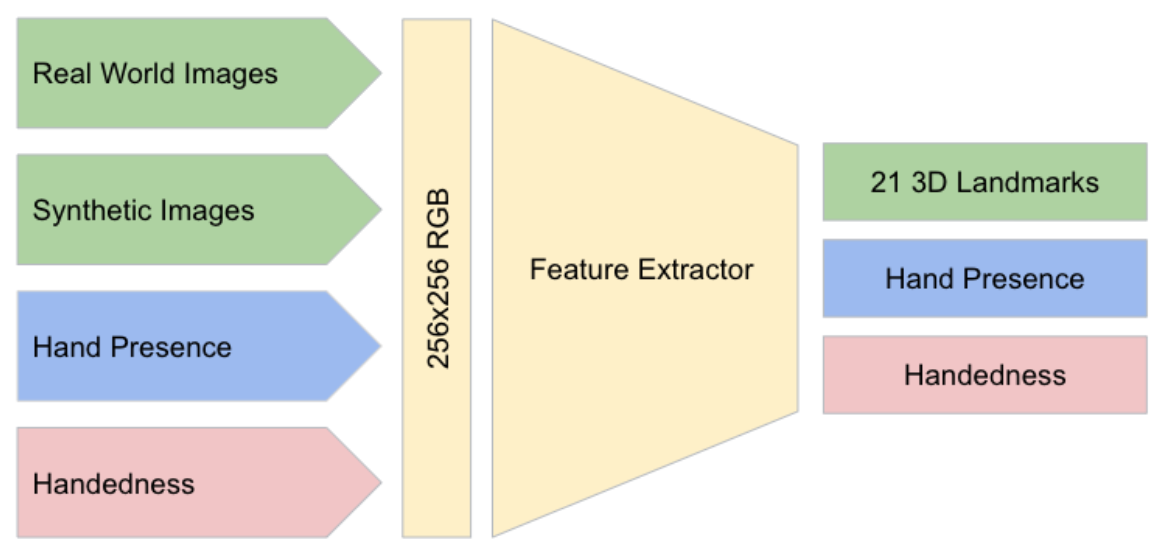
\includegraphics[width=0.7\textwidth]{landmark.png}
    \caption[معماری مدل نقطه عطف دست]{معماری مدل نقطه عطف دست. این مدل دارای سه خروجی است که یک استخراج کننده ویژگی را به اشتراک می‌گذارند. هر سر توسط مجموعه داده های مربوطه که با همان رنگ مشخص شده اند آموزش داده می‌شود \cite{zhang2020mediapipe}.}
\end{figure}

\begin{figure}[h]
    \centering
    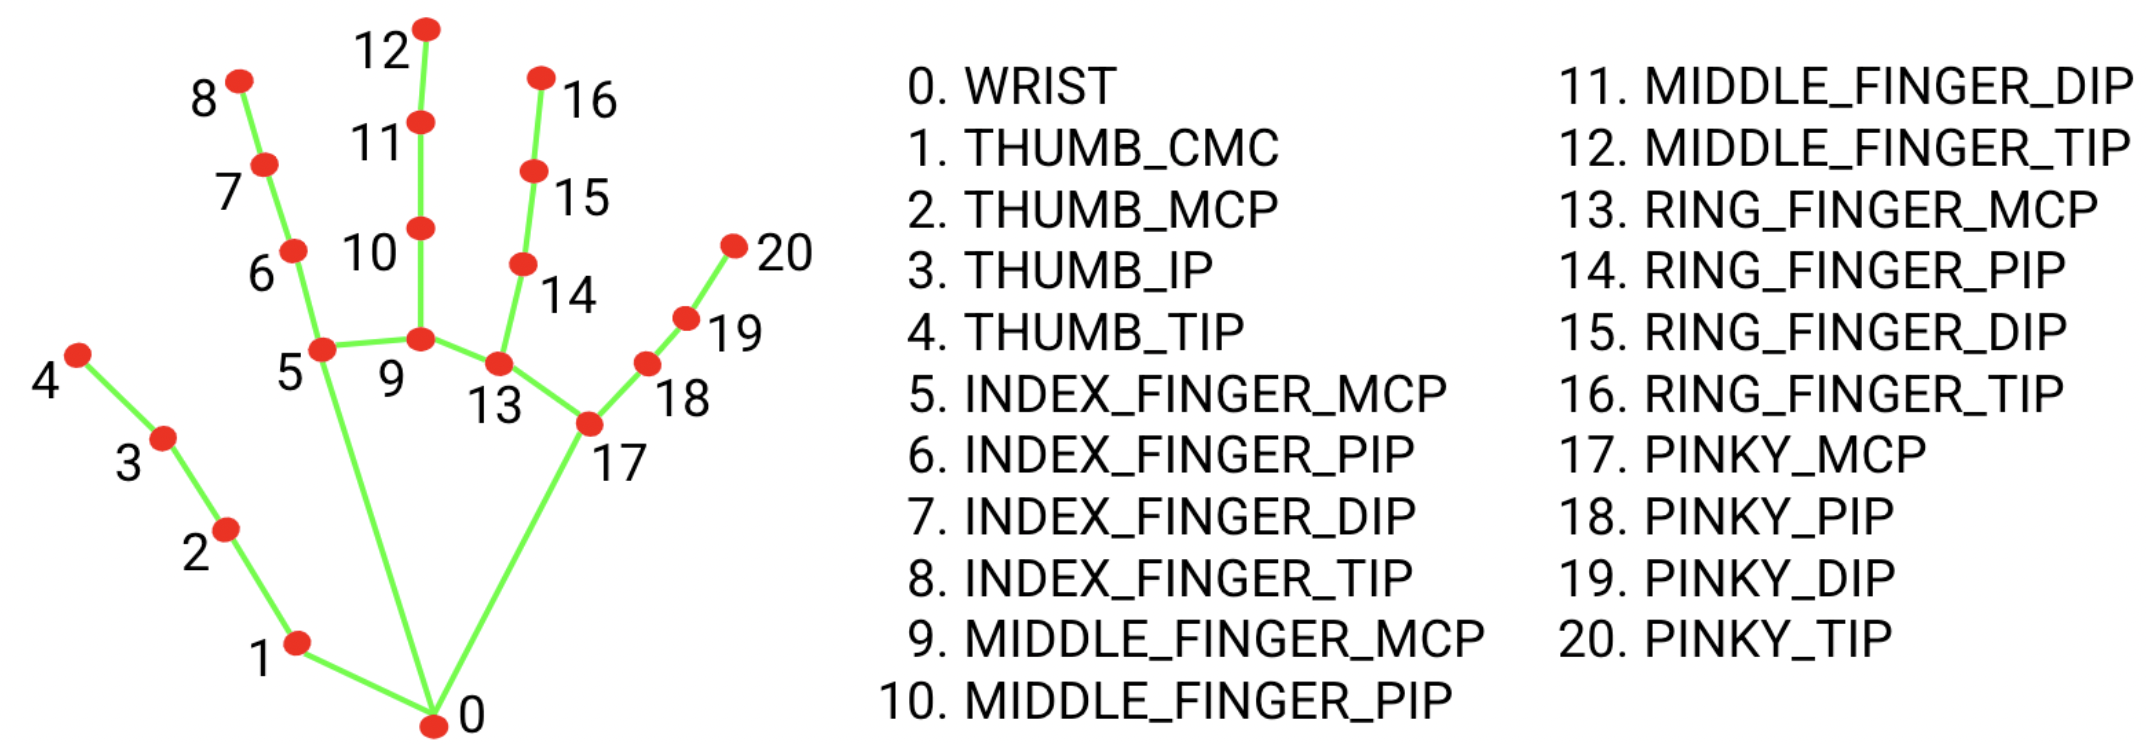
\includegraphics[width=1\textwidth]{hand-landmarks.png}
    \caption[موقعیت ۲۱ نقطه کلیدی در ناحیه دست]{موقعیت ۲۱ نقطه کلیدی در ناحیه دست \cite{zhang2020mediapipe}}
\end{figure}

\subsection{برش تصویر \protect\LTRfootnote{Image Cropping}}
ماژول برش تصویر برای برش و استخراج ناحیه‌های مورد نظر از تصاویر استفاده می‌شود. این ماژول ورودی‌هایی مانند تصویر اصلی و جعبه مرزی\LTRfootnote{Bounding Box} یا مختصات برش را می‌پذیرد و تصویر برش‌خورده حاوی ناحیه مورد 
نظر را تولید می‌کند. معماری این ماژول شامل مراحل پیش‌پردازش، عملیات برش\LTRfootnote{Cropping Operation}  و پس‌ پردازش  می‌باشد. وظیفه اصلی این ماژول برش دقیق ناحیه‌های مورد نظر از تصویر اصلی است که در کاربردهای 
مختلفی مانند پیش‌پردازش برای تشخیص چهره یا دست، تحلیل تصاویر پزشکی، واقعیت افزوده و پردازش تصویر در کاربردهای امنیتی مورد استفاده قرار می‌گیرد. این ماژول به 
توسعه‌دهندگان این امکان را می‌دهد که ناحیه‌های خاصی از تصاویر را به‌صورت دقیق و مؤثر استخراج کرده و برای پردازش‌های بعدی آماده کنند \cite{zhang2020mediapipe}.

\subsection{نقاط عطف یه مستطیل\protect\LTRfootnote{Landmarks To Rectangle}}
این ماژول برای تبدیل نقاط کلیدی به مستطیل‌های محدودکننده استفاده می‌شود. هدف آن محصور دقیق نقاط کلیدی دست است. با استفاده از این مستطیل‌ها، می‌توان موقعیت دقیق‌تر اشیاء در 
تصویر را نمایش داد و از آن‌ها به عنوان ورودی برای ماژول‌های بعدی در گراف استفاده کرد. این ماژول شامل مراحل پیش‌پردازش داده‌های ورودی، محاسبه مستطیل محدودکننده، نرمال‌سازی مختصات مستطیل‌ها و تولید خروجی نهایی 
 می‌باشد. وظیفه اصلی این ماژول تبدیل نقاط کلیدی به مستطیل‌های محدودکننده‌ی دقیق است که در بسیاری از کاربردها اهمیت دارد، از جمله آن‌ها ردیابی اشیاء، تحلیل حرکات، پیش‌پردازش برای مدل‌های دیگر و افزایش دقت در پردازش تصویر است \cite{zhang2020mediapipe}.
تفاوت این ماژول با ماژول اول این است که در ماژول اول ما ورودی خام از تصاویر و یا فریم‌های ویدیو را به عنوان ورودی داده و محدوده‌ی دست را تعیین ‌می‌کنیم, اما در 
این ماژول نقاط کلیدی استخراج شده به ماژول داده می‌شوند تا مجدد یک مستطیل محدودکننده برای نقاط عطف استخراح شده تولید کند.

% \subsection{ارائه کننده حاشیه نویسی\protect\LTRfootnote{Annotation Renderer}}
% این ماژول برای نمایش گرافیکی نتایج پردازش‌های مختلف بر روی تصاویر یا ویدیوها استفاده می‌شود. این ماژول اطلاعات حاشیه‌نویسی شامل نقاط کلیدی، مستطیل‌های محدودکننده، خطوط، متن و سایر اشکال گرافیکی را به صورت 
% بصری بر روی تصاویر نمایش می‌دهد. وظیفه اصلی آن شامل نمایش بصری نقاط کلیدی، مستطیل‌های محدودکننده، خطوط و اتصالات، متن و توضیحات بر روی تصاویر یا ویدیوها است. این ماژول به توسعه‌دهندگان امکان 
% می‌دهد تا به راحتی و به صورت بصری نتایج پردازش‌های خود را مشاهده کنند و از این طریق به بهبود و ارزیابی عملکرد مدل‌ها و الگوریتم‌های خود بپردازند.
% همچنین وجود این ماژول توضیح پذیری مدل‌های یادگیری عمیق استفاده شده را نیز افزایش می دهد
% \cite{zhang2020mediapipe}.

\section{پیش‌بینی علائم دست}
% \subsection{مدل پیش‌بینی علائم دست}  
برای پیش‌بینی علائم دست از مدل‌های گوناگونی استفاده شده است که معماری و مشخصات هر یک در ادامه به تفکیک توضیح داده‌ شده‌اند. این معماری‌ها شامل شبكه چندلایه‌ای پرسپترونی، شبكه عصبي پیچشی، شبكه عصبي بازگشتي و شبكه‌هاي حافظه كوتاه مدت بلند مدت است. دلیل استفاده از این مدل‌ها حجم کم و در عین حال دقت بالای آن‌ها است تا بتوان آن‌ها را با یکدیگر قیاس و در نهایت بهترین مدل را برگزید. 
ورودی این مدل، نقاط کلیدی دست و خروجی آن پس از پردازش، شامل ۱۰ کلاس است. شایان ذکر است که کاربر توانایی اضافه کردن کلاس و در نتیجه علائم جدید را نیز در صورتی که پهپاد قابلیت انجام آن را داشته باشد دارد.


\begin{figure}[h]
    \centering
    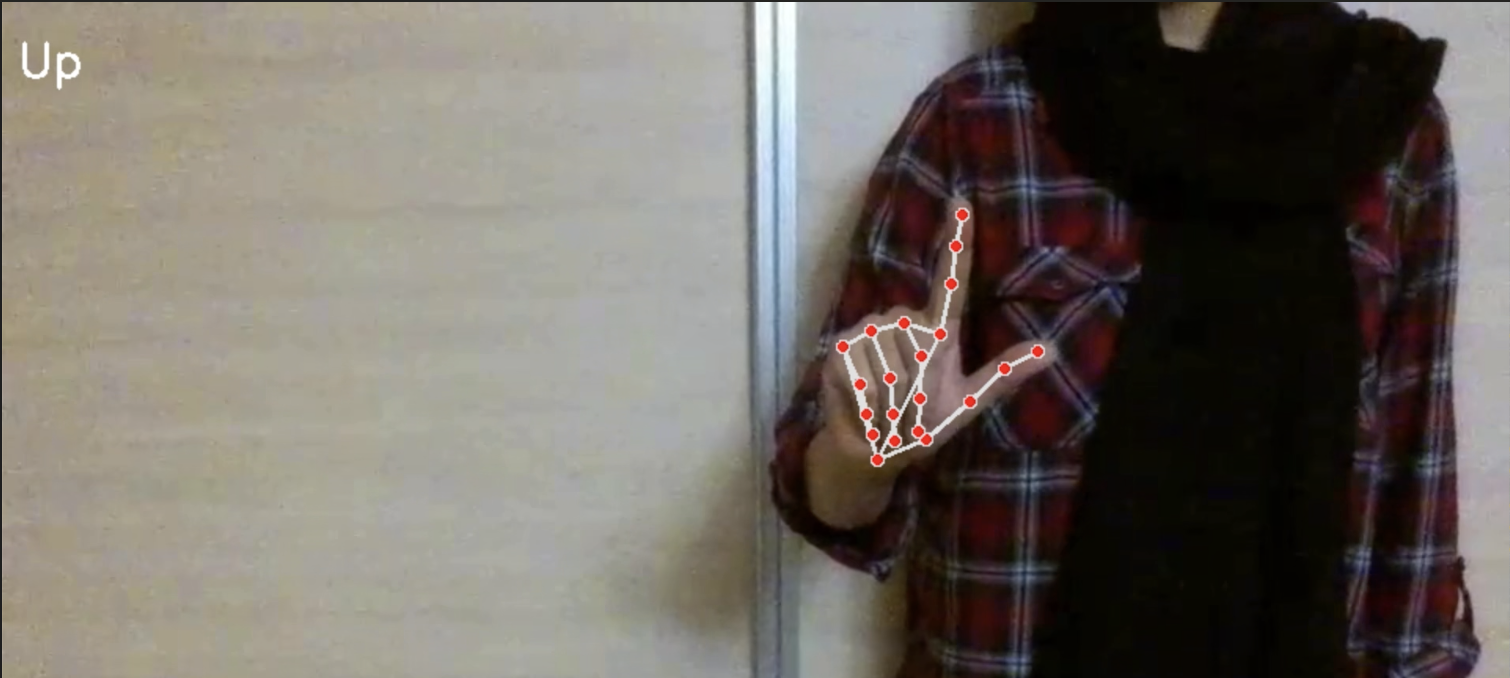
\includegraphics[width=0.7\textwidth]{gesture_UP.png}
    \caption {نمونه پیش‌بینی علامت دست}
\end{figure}



% \begin{figure}[h]
%     \centering
%     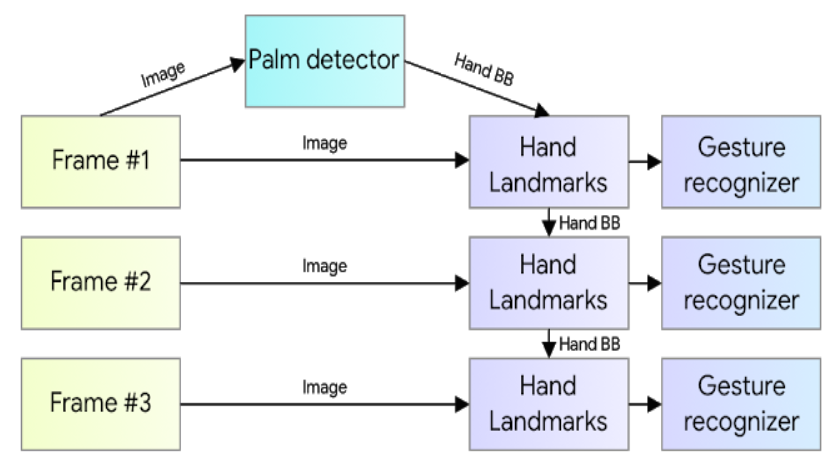
\includegraphics[width=0.7\textwidth]{mediapipe.png}
%     \caption[خط لوله تشخیص علائم دست]{خط لوله تشخیص علائم دست \cite{zhang2020mediapipe}}
% \end{figure}



\subsection{مدل‌های ماژول کلاس‌بندی برای تعیین علائم دست}

\subsubsection{شبکه عصبی  چندلایه‌ای پرسپترونی}
شبکه عصبی  چندلایه‌ای پرسپترونی \LTRfootnote{Multilayer Perceptron Neural Network} نوعی شبکه عصبی  هوش مصنوعی است که از چندین لایه نورون تشکیل شده است. نورون‌های درون لایه‌ها معمولاً از
توابع فعال‌سازی غیرخطی \LTRfootnote{Nonlinear Activation Functions} استفاده می‌کنند که به شبکه اجازه می‌دهد الگوهای پیچیده در داده‌ها را بیاموزد. شبکه‌های عصبی چندلایه‌ای پرسپترونی در 
یادگیری ماشین اهمیت بالایی دارند زیرا می‌توانند روابط غیرخطی در داده‌ها را یاد بگیرند و آن‌ها را به مدل‌های قدرتمندی برای استفاده در کارهایی مانند طبقه‌بندی، رگرسیون و تشخیص الگو تبدیل کند. 
\\
شبکه عصبی چندلایه‌ای پرسپترونی نوعی شبکه عصبی پیش‌خور\LTRfootnote{Feedforward} است که از نورون‌های کاملاً متصل با یک تابع فعال‌سازی از نوع غیر خطی تشکیل شده است و  برای تشخیص داده‌هایی که به صورت خطی قابل تفکیک نیستند استفاده می‌شود.
\\
شبکه‌های عصبی چندلایه‌ای پرسپترونی به طور گسترده در زمینه‌های مختلف از جمله تشخیص تصویر، پردازش زبان طبیعی و تشخیص گفتار و ... استفاده می‌شوند. انعطاف پذیری آن‌ها در
معماری و توانایی تقریب هر عملکرد تحت شرایط خاص آن‌ها را به یک بلوک اساسی در یادگیری عمیق و تحقیقات شبکه عصبی تبدیل می‌کند. 

\begin{figure}[h]
    \centering
    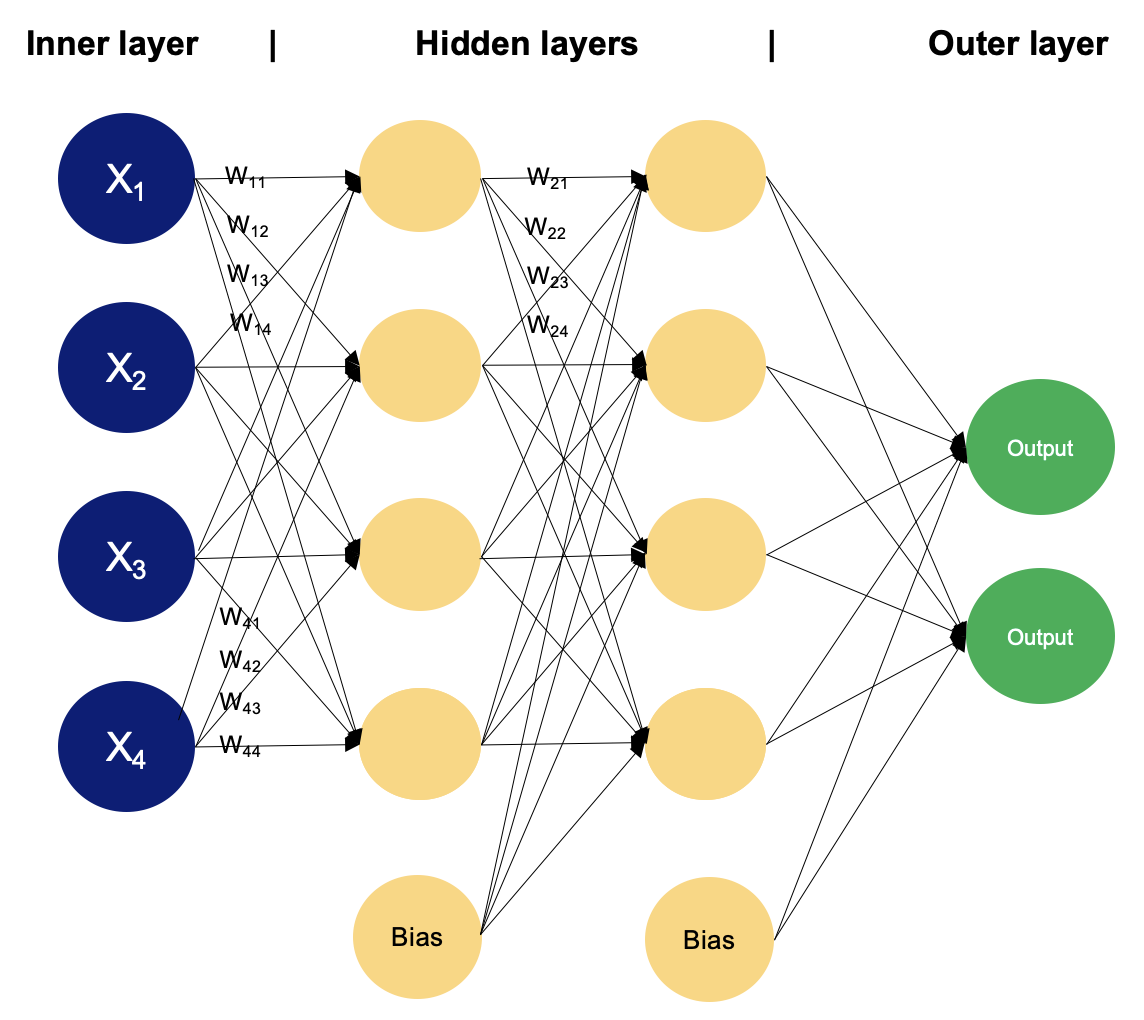
\includegraphics[width=0.6\textwidth]{MLP.png}
    \caption[نمونه ای از شبکه‌های عصبی چند لایه‌ای دارای دو لایه پنهان]{نمونه ای از شبکه‌های عصبی چند لایه‌ای دارای دو لایه پنهان\cite{Multilay58:online}}
\end{figure}


\subsubsection{شبکه‌ عصبی پیچشی}
شبکه‌های عصبی پیچشی\LTRfootnote{Convolutional Neural Network} یک الگوریتم یادگیری عمیق است که از جمله کاربرد‌های آن در زمینه‌ی تشخیص اشیا می‌توان به مواردی مانند طبقه بندی، تشخیص و تقسیم بندی تصویر 
اشاره کرد. بسیاری از برنامه‌های کاربردی مانند اتومبیل های خودران، دوربین های نظارتی و موارد دیگر از شبکه‌های عصبی پیچشی استفاده می‌کنند.
\\
برخلاف مدل‌های سنتی یادگیری ماشین مانند ماشین بردار پشتیبانی و درخت‌ تصمیم
\LTRfootnote{Decision Tree}
که نیاز به استخراج دستی ویژگی‌ها دارند، شبکه‌های عصبی پیچشی می‌توانند استخراج خودکار ویژگی‌ها را در مقیاس‌های بزرگ 
انجام دهند. این ویژگی یکی از دلایل اصلی کارآمد بودن این شبکه‌ها است. این شبکه‌ها می‌توانند الگوهای مختلف را از درون داده‌ها تشخیص دهند و ویژگی‌های داده را بدون توجه به موقعیت آن‌ها، اعم از چرخش، تبدیل‌‌های هندسی و یا جابجایی تصاویر استخراج کنند.
\\
معماری شبکه‌های عصبی پیچشی سعی می‌کنند تا ساختار نورون‌ها را در سیستم بینایی انسان متشکل از چندین لایه تقلید کند، جایی که هر یک مسئول تشخیص یک ویژگی خاص در داده‌ها است. 
همانطور که در 
\cref{cnn_arch}
نیز نشان داده شده است، شبکه عصبی پیچشی از چندین لایه مانند لایه ورودی، لایه پیچشی، لایه ادغام \LTRfootnote{Pooling} و لایه‌های کاملاً متصل تشکیل شده است.
\\
لایه پیچشی فیلترهایی را روی تصویر ورودی اعمال می‌کند تا ویژگی‌ها را استخراج کند, لایه ادغام ابعاد تصویر را کاهش می‌دهد تا محاسبات را سریع‌تر و کمتر کند و لایه کاملاً متصل پیش بینی نهایی را انجام می‌دهد. بدین صورت که شبکه فیلترهای بهینه را از طریق پس انتشار
\LTRfootnote{Back Propagation}
و نزول گرادیان
\LTRfootnote{Gradian Descent}
می‌آموزد.


\begin{figure}[h]
    \centering
    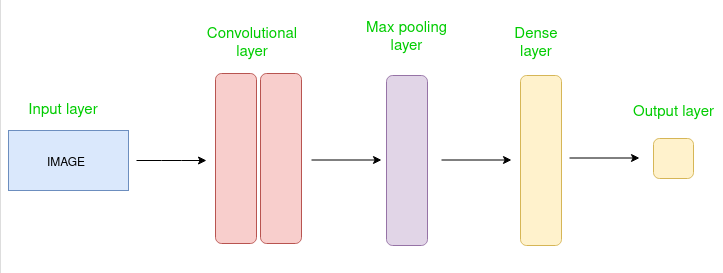
\includegraphics[width=0.9\textwidth]{CNN_arch.png}
    \caption[نمونه معماری شبکه عصبی پیچشی]{نمونه معماری شبکه عصبی پیچشی \cite{Introduc84:online}}\label{cnn_arch}
\end{figure}


\subsubsection{شبکه عصبی بازگشتی}
شبکه عصبی بازگشتی\LTRfootnote{Recurrent Neural Network}  نوعی شبکه عصبی است که در آن خروجی مرحله قبل به عنوان ورودی به مرحله فعلی داده می‌شود. در شبکه‌های عصبی سنتی، تمامی ورودی‌ها و خروجی‌ها مستقل از یکدیگر 
هستند. برای مثال در مواردی که پیش‌بینی مدل متکی به موارد قبلی است و نیاز است آن‌ها را نیز مدنظر قرار دهد این شبکه بسیار کارآمد است. شبکه عصبی بازگشتی با کمک یک لایه پنهان این امکان را فراهم می‌کند. اصلی‌ترین و مهم‌ترین 
ویژگی شبکه عصبی بازگشتی حالت پنهان آن است که برخی از اطلاعات یک دنباله را به خاطر می‌سپارد. این حالت به عنوان حالت حافظه نیز شناخته می‌شود زیرا ورودی قبلی شبکه را به خاطر می‌آورد. و از پارامترهای یکسانی برای هر 
ورودی استفاده می‌کند چرا که وظیفه یکسانی را روی تمام ورودی‌ها یا لایه‌های پنهان برای تولید خروجی انجام می‌دهد. این بر خلاف سایر شبکه‌های عصبی، پیچیدگی پارامترها را کاهش می‌دهد.


\begin{figure}[h]
    \centering
    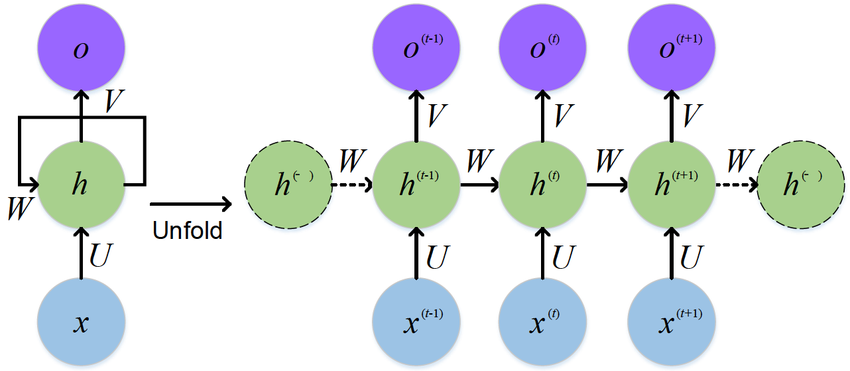
\includegraphics[width=0.8\textwidth]{RNN.png}
    \caption[نمونه معماری شبکه عصبی بازگشتی]{نمونه معماری شبکه عصبی بازگشتی\cite{inproceedings}}
\end{figure}

\subsubsection{شبکه‌ حافظه طولانی کوتاه مدت}
شبکه عصبی بازگشتی یک حالت پنهان دارد که در طول زمان منتقل می‌شود، این مساله می‌تواند یادگیری وابستگی‌های طولانی مدت را برای شبکه دشوار کند. شبکه‌های حافظه طولانی کوتاه مدت
\LTRfootnote{Long Short-Term Memory }
این مشکل را با معرفی یک سلول حافظه برطرف می‌کند، این سلول محفظه‌ای است که می‌تواند اطلاعات را برای مدت طولانی نگهداری کند. شبکه‌های حافظه طولانی کوتاه مدت 
 قادر به یادگیری وابستگی‌های طولانی‌مدت در داده‌های متوالی هستند، که آن‌ها را برای کارهایی مانند ترجمه زبان، تشخیص گفتار و پیش‌بینی 
سری‌های زمانی مناسب می‌سازد. شبکه‌های حافظه طولانی کوتاه مدت همچنین می توانند در ترکیب با دیگر معماری‌های شبکه عصبی، مانند شبکه‌های عصبی پیچشی برای تجزیه و تحلیل تصویر و ویدئو استفاده شوند.
\\
سلول حافظه توسط سه گیت کنترل می‌شود: گیت ورودی، دروازه فراموشی و گیت خروجی. این گیت‌ها تصمیم می‌گیرند که چه اطلاعاتی را به سلول حافظه اضافه، حذف  و از آن خروجی بگیرند. گیت ورودی کنترل می‌کند که چه اطلاعاتی 
به سلول حافظه اضافه می‌شود. دروازه فراموشی کنترل می‌کند که چه اطلاعاتی از سلول حافظه حذف می‌شود. و گیت خروجی کنترل می‌کند که چه اطلاعاتی از سلول حافظه خارج می‌‌شود.
این  گیت به شبکه‌های حافظه طولانی کوتاه مدت اجازه می‌دهد تا به‌طور انتخابی اطلاعات در جریان درون شبکه را حفظ  و یا کنار بگذارند. این ویژگی امکان آموزش وابستگی‌های طولانی‌مدت را برای شبکه فراهم می‌کند .

\begin{figure}[h]
    \centering
    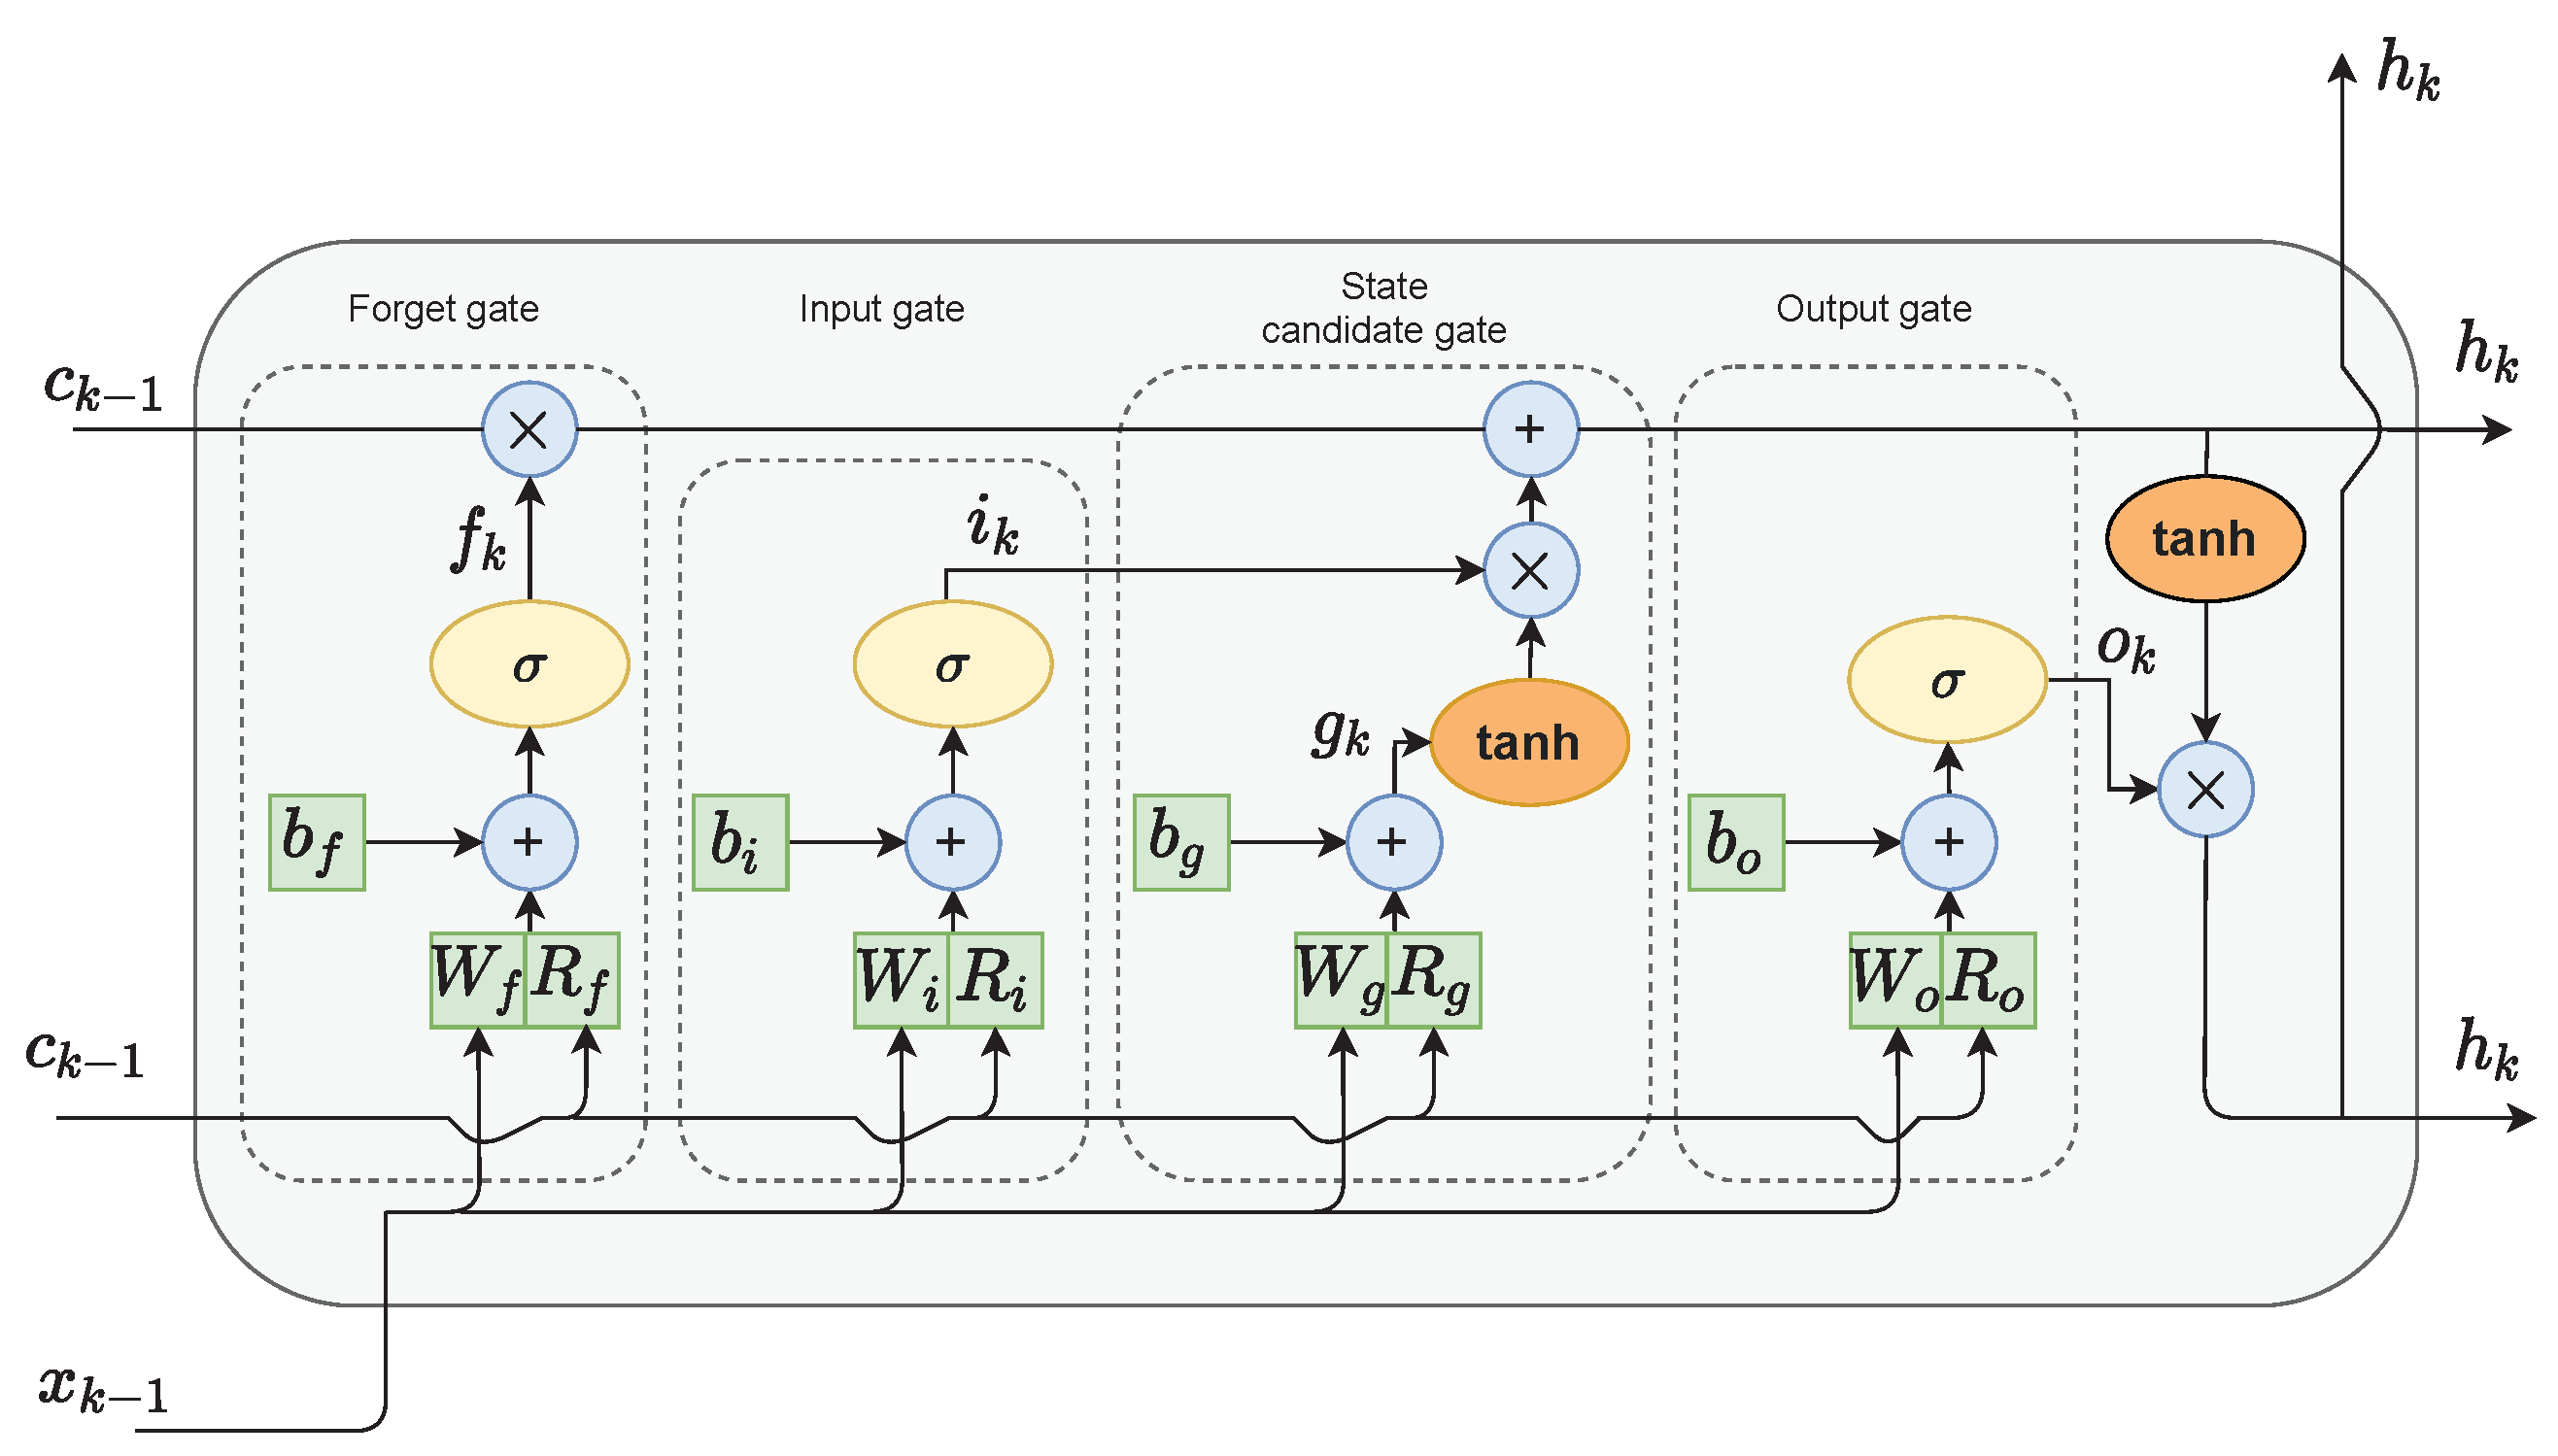
\includegraphics[height=9cm,width=0.9\textwidth]{LSTM.png}
    \caption[نمونه معماری شبکه‌ حافظه طولانی کوتاه مدت]{نمونه معماری شبکه‌ حافظه طولانی کوتاه مدت \cite{s21165625}}
\end{figure}




\subsection{پیش‌پردازش داده‌ها}
برای ورود نقاط عطف دست به مدل تعیین علائم، به ۲۱ مختصات طول و عرض نیاز داریم. خروجی مدل تعیین مختصات نقاط عطف دست برابر مختصات مطلق پیکسل‌ها نسبت به گوشه سمت 
چپ پایین تصویر است. این نقاط با توجه به اندازه عکس می‌توانند گسترده باشند برای مثال در یک عکس با اندازه ۲۰۴۸*۲۰۴۸ این اعداد از بین ۰ تا ۲۰۴۸ متغیر اند. 
اگر این مختصات را به صورت مستقیم به مدل تعیین علائم دست بدهیم دقت مدل برابر ۸۷ درصد خواهد بود که به میزان کافی مورد قبول نیست. برای بهبود آن باید پیش‌پردازش‌هایی بر روی داده ورودی انجام شود. 
\\
از جمله این پیش‌پردازش‌ها می‌توان به نسبی کردن و نرمال‌سازی داده‌ها اشاره کرد. برای این کار ابتدا باید یک مرجع واحد در نظر گرفت تا نقاط، نسبت به آن مشخص شوند. در این پروژه ما مرجع را نقطه 
مشخص شده روی مچ در نظر می‌گیریم. مختصات نقطه مرجع را برابر (0,0)  قرار می‌دهیم. سپس نسبت به آن و با توجه به
\cref{eq:ref}
مختصات نقاط دیگر را به روز رسانی می‌کنیم.

\begin{equation}\label{eq:ref}
    X_{rel} = X_ref -X
\end{equation}


پس از نسبی کردن نقاط نسبت به مبدأ، آن‌ها را با کمک 
\cref{eq:normal_ref}
نرمال سازی می‌کنیم تا تمام طول و عرض نقاط به عددی میان صفر و یک به روز رسانی شوند.
\begin{equation}\label{eq:normal_ref}
    X_{new} = \frac{X - X_{min}}{X_{max} - X_{min}}
\end{equation}

در انتها این این مختصات را به عنوان ورودی به شبکه تعیین علائم دست می‌دهیم. با توجه به اینکه معماری هیچ یک از مدل‌ها تغییر نکرده است و تنها داده‌های مختصات به روز رسانی شده‌اند، 
دقت نهایی مدل به ۹۷ درصد افزایش پیدا کرده است و پیش‌پردازش تاثیر به‌سزایی در افزایش دقت پروژه داشته است.


\subsection{رأی‌گیری پنجره‌ای}
% \subsection{پس‌پردازش}
با وجود اینکه دقت مدل پیاده‌سازی شده بالا و مقدار قابل قبولی است و عملکرد بسیار چشم‌گیری از خود نشان می‌دهد، در عین حال پیش‌بینی اشتباه مدل می‌تواند عواقب زیان‌باری را به ارمغان آورد، 
از تجربه ناپسند برای کاربر گرفته تا برخورد پهپاد به اجسام و هزینه‌های مالی گزاف. لذا باید دقت انجام پروژه را از آنچه مدل پیش‌بینی می‌کند نیز بالاتر برد. برای این کار از رأی‌گیری پنجره‌ای 
استفاده کرده‌ایم. بدین صورت که متغیری را با توجه به تعداد فریم بر ثانیه دوربین در نظر می‌گیریم، هر چه تعداد فریم ضبط شده بر ثانیه در دوربین پهپاد بیشتر باشد متغیر در نظر گرفته‌شده نیز بیشتر 
است. در این پروژه از آنجایی که نرخ فریم بر ثانیه دوربین پهپاد برابر با سی است.  مقدار این متغیر را برابر با ده در نظر می‌گیریم.  سپس یک حد بالا بین صفر تا یک برای تایید خروجی
 نهایی تعریف می‌کنیم. مقدار این متغییر نیز در این پروژه برابر با 7.0 در نظر گرفته شده است . طبق این راه ما ده فریم متناوب گرفته‌شده از پهپاد را به مدل پیاده‌سازی شده می‌دهیم اما تنها در صورتی دستور پیش‌بینی شده را به 
پهپاد می‌دهیم که حد ممکن را بدست آورد. برای مثال اگر هفت یا بیشتر از ده حرکت پیش بینی شده، دستور حرکت رو به جلو باشد آنگاه به پهپاد دستور داده می‌شود تا به جلو حرکت کند. 
در غیر این صورت اگر کمتر از هفت عدد از فریم‌ها یک   حرکت یکسانی از دست را پیش‌بینی نکنند، پهپاد در حالت قبلی خود باقی می‌ماند و دستوری به آن داده نمی‌شود.

\begin{figure}[h]
    \centering
    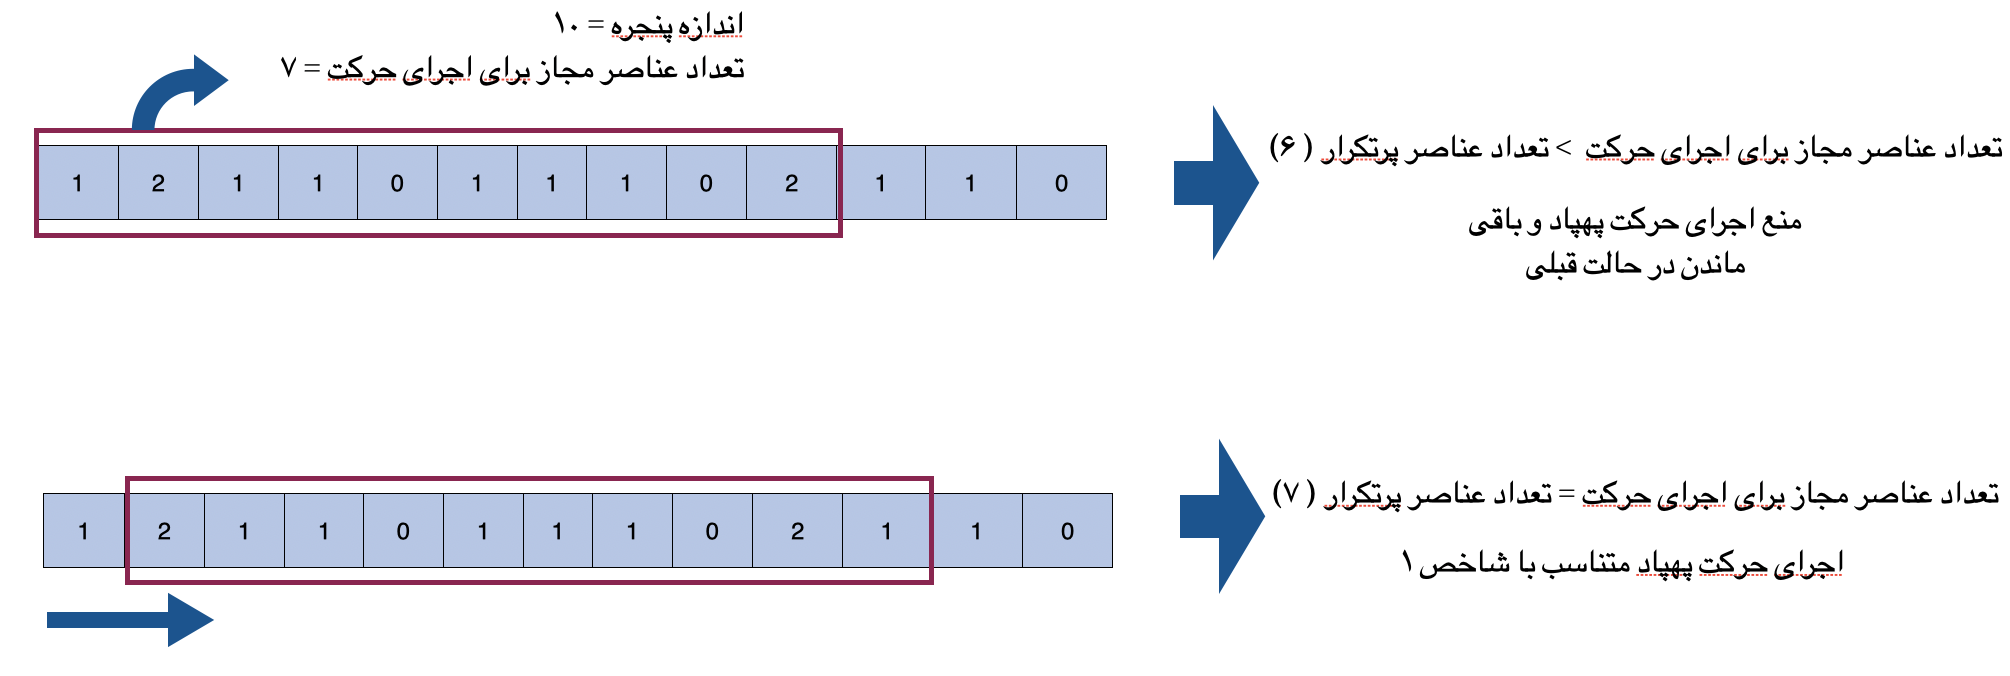
\includegraphics[width=1\textwidth]{window.png}
    \caption{نمونه رأی‌گیری پنجره‌ای موفق و ناموفق}
\end{figure}

\section{ارتباط با پهپاد دی‌جی‌آی تلو}
پهپاد دی‌جی‌آی تلو یکی از پهپادهای کوچک و هوشمند است که به عنوان یک ابزار آموزشی و پژوهشی در زمینه مهندسی کنترل مورد استفاده قرار می‌گیرد. از آنجایی که دی‌جی‌آی تلو دارای سنسور دوربین، سنسور واحد اندازگیری اینرسی \LTRfootnote{Inertial Measurement Unit} 
و سایر سنسورهای مفید برای جمع آوری داده ها برای تحلیل و کنترل در زمان واقعی است، این پهپاد به عنوان یک پلتفرم آموزشی بسیار مناسب برای پیاده‌سازی پروژه ما در نظر گرفته می‌شود.
\\
ارتباط این پهپاد با مدل هوش مصنوعی که توسط برنامه پایتون نوشته شده‌است، با کمک کتاب‌خانه دی‌جی‌آی تلوپی برقرار می‌شود. این کتاب‌خانه دستورات ابتدایی، که پهپاد توانایی انجام آنها را دارد به صورت دستورالعمل‌های بسیار ساده پیاده‌سازی کرده است. در ابتدای اجرای برنامه، با کمک دستورهای کتاب‌خانه دوربین روشن شده و پهپاد بلند می‌شود. سپس در هر لحظه
 دوربین تصاویر گرفته‌شده را با کمک ارتباط بی‌سیم به سرور مربوطه می‌فرستد. در ادامه مدل پیاده‌شده با پردازش تصویر، علامت مربوط به دست را پیش‌بینی می‌کند و با ارتباط بی‌سیم و دستورالعمل مناسب فرمان را به پهپاد ارسال می‌کند.
 \\
 از جمله دستورهایی از این کتابخانه که در پروژه استفاده شده‌اند در جدول \ref{table:commands} ذکر شده‌است.

\begin{table}[h!]
    \centering
    \begin{tabular}{||>{\centering\arraybackslash}p{4cm} >{\centering\arraybackslash}p{11.5cm}||}
     \hline
    \rule{0pt}{3ex} حرکت پهپاد & دستورالعمل \\ [1.5ex]
    \hline
     \rule{0pt}{0.5ex} & \\  
     وصل شدن به پهپاد & \text{\lr{connect()}} \\ [2.5ex]
     روشن کردن دوربین & \text{\lr{streamon()}} \\ [2.5ex]
     بلند شدن & \text{\lr{takeoff()}} \\ [2.5ex]
     گرفتن فریم‌ها از دوربین & \text{\lr{get\text{\_}frame\text{\_}read()}} \\ [2.5ex]
     حرکت به ۶ جهت اصلی & \text{\lr{send\text{\_}rc\text{\_}control(left\text{\_}right, forward\text{\_}backward, up\text{\_}down, yaw)}} \\ [2.5ex]
     چرخش ساعتگرد & \text{\lr{rotate\text{\_}counter\text{\_}clockwise(degree)}} \\ [2.5ex]
     فرود آمدن & \text{\lr{land()}} \\ [2.5ex]
     خاموش کردن دوربین & \text{\lr{streamoff()}} \\ [2.5ex]
     قطع ارتباط با پهپاد& \text{\lr{end()}} \\ [2.5ex]
     \hline
    \end{tabular}
    \caption{لیست دستورالمعل‌های استفاده شده در کتاب‌خانه دی‌جی‌آی تلوپی برای ارتباط با پهپاد}
    \label{table:commands}
\end{table}


\section{پیاده‌سازی میدانی پروژه}
پس از پیاده‌سازی تمام اجزای پروژه و رسیدن به دقت بالا، این پروژه بر روی پهپاد دی‌جی‌آی تلو به اجرا در آمده‌است. 
تصویر \ref{phisical} قسمتی از اجرای میدانی پروژه است که در لینک \href{https://github.com/sara-tajernia/hand-gesture-control_drone}{گیت‌هاب} و \href{https://www.aparat.com/v/chgtnhm}{آپارات} ویدیو کامل آن قابل مشاهده است.



\begin{figure}[h]
    \centering
    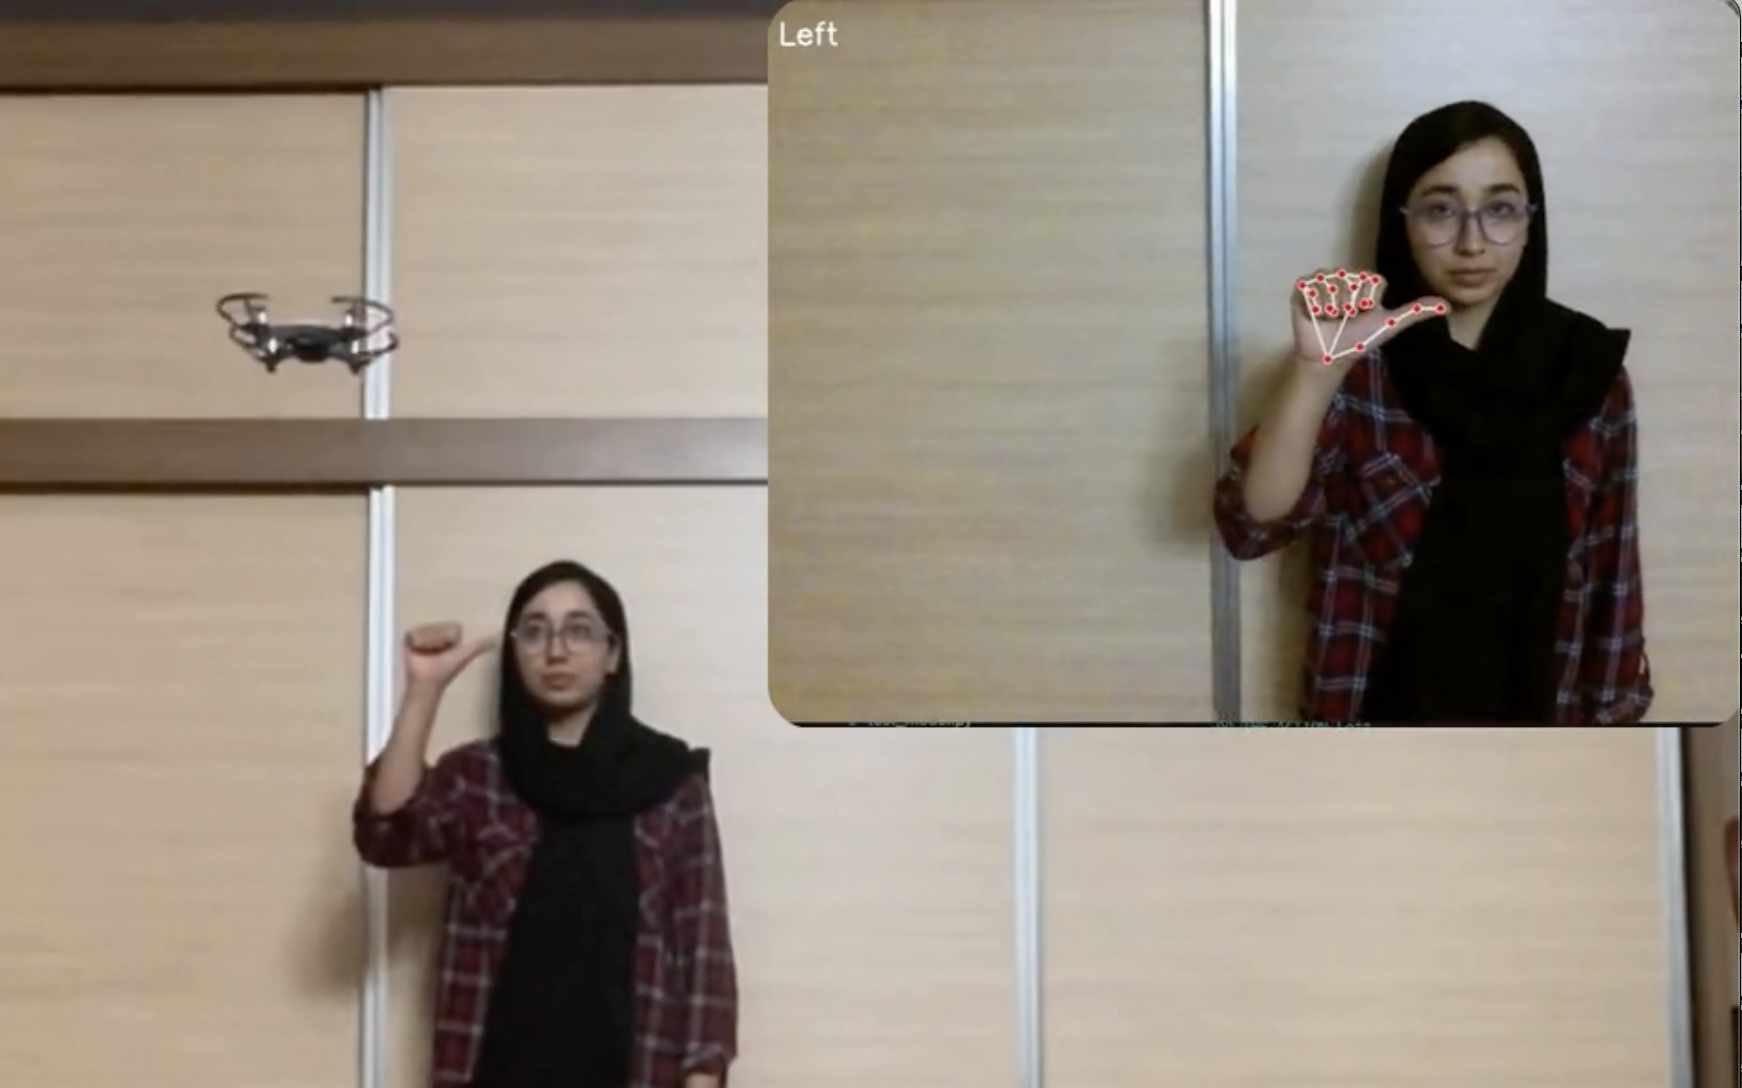
\includegraphics[width=0.8\textwidth]{drone_control.png}
    \caption{نمونه تصویر پیاده‌سازی مدل بر روی پهپاد دی‌جی‌آی تلو}
    \label{phisical}
\end{figure}

\section{جمع‌بندی}
در این فصل قسمت‌های مختلف پیاده‌سازی شده پروژه با جزئیات کامل توضیح داده شد. که این توضیحات شامل نرم‌افزار‌ها و سخت‌افزارها، کتاب‌خانه‌ها، پیش‌پردازش، پس‌پردازش و کد اصلی که شامل سه مدل به صورت پی در پی است می‌شود.
دو مدل از این سه مدل وظیفه استخراج ویژگی‌ها و نقاط کلیدی دست و مدل آخر نیز وظیفه کلاس‌بندی علائم ورودی داده شده را دارند.
در فصل بعدی به بررسی نتایج به دست آمده از این معماری پیشنهاد شده و ارزیابی و مقایسه معماری خود با دیگر کار‌های مشابه می‌پردازیم.



\chapter{نتایج و ارزیابی}
\section{مقدمه}
سیستم تشخیص حرکات دست نقش مهمی در زمینه ایجاد تعامل کارآمد بین انسان و ماشین ایفا می‌کند. پیاده‌سازی این سیستم با استفاده از تشخیص علائم دست، باعث افزایش وسیعی در استفاده کاربردی از هوش مصنوعی  در صنعت فناوری می‌شود. در این پروژه، 
معماری‌های گوناگونی مانند شبکه‌های عصبی پیچشی، شبکه‌های حافظه کوتاه‌مدت بلند، و شبکه‌های عصبی چندلایه‌ای پرسپترونی مورد آزمایش قرار گرفتند تا بهترین پیاده‌سازی برای تشخیص حرکات دست انتخاب شود. 
\\
در این فصل، به بررسی نتایج به‌دست‌آمده از این پیاده‌سازی‌های متفاوت می‌پردازیم و دقت و عملکرد سیستم در شرایط مختلف را ارزیابی می‌کنیم. همچنین، نقاط قوت و ضعف هر یک از معماری‌های مورد استفاده 
را تحلیل کرده و پیشنهاداتی برای بهبود سیستم ارائه می‌دهیم. هدف این فصل، ارائه یک تحلیل جامع از کارایی سیستم و شناخت دقیق‌تر از عواملی است که می‌توانند به ارتقاء عملکرد آن کمک کنند.

\section{ارزیابی عملکرد مدل‌ها}

این پروژه با مدل‌های گوناگونی پیاده‌سازی شده است تا بتوان بهترین آنها را برای نتیجه نهایی بر روی پهپاد اجرا کرد. معیارهای ارزیابی شامل دقت، صحت \LTRfootnote{Precision}، فراخوانی\LTRfootnote{Recall}، امتیاز \lr{F1} و
تعداد نمونه‌ها برای هر یک از علائم‌ می‌باشد.
\\
معیار‌های دقت، صحت، فراخوانی و امتیاز \lr{F1} معیارهای ضروری برای ارزیابی عملکرد مدل‌های بینایی ماشین و یادگیری عمیق هستند. این معیار‌ها هر دو نتیجه مثبت کاذب و منفی کاذب را در نظر
می‌گیرند و درک دقیقی از قابلیت‌های پیش بینی یک مدل را ارائه می‌دهند. این ارزیابی دقیق با برجسته کردن نقاط قوت و ضعف خاص هر مدل, به اصلاح مدل کمک می‌کند.
\subsection{دقت}
دقت مدل معیاری است که نشان می‌دهد یک مدل یادگیری عمیق تا چه اندازه قادر به پیش‌بینی یا تصمیم‌گیری صحیح بر اساس داده‌ها است. این معیار به صورت نسبت مجموع مثبت و منفی واقعی به تعداد کل نمونه‌ها محاسبه می‌شود.
\\
دقت، بصری‌ترین معیار عملکرد است و به نسبت مشاهدات پیش‌بینی شده صحیح به کل مشاهدات اشاره دارد. این معیار برای مقایسه عملکرد مدل‌های مختلف و ارزیابی اثربخشی یک مدل خاص برای یک وظیفه معین استفاده می‌شود. دقت زمانی مناسب است که توزیع کلاس‌ها متعادل باشد و هزینه‌ نتیجه‌های مثبت کاذب و منفی کاذب مشابه باشند \cite{Accuracy53:online}.
\begin{equation}
    Accuracy = \frac{True \, Positives + True \, Negatives}{True \, Positives + True \, Negatives + False \, Positives + False \, Negatives}
\end{equation}


\begin{table}[h!]
    \centering
    \begin{tabular}{||c c c c||}
     \hline
     \rule{0pt}{3ex} معماری مدل & دوره & دقت داده آموزش & دقت داده تست  \\ [1.5ex]
     \hline
     \hline
     \rule{0pt}{0.5ex} & & & \\  
     شبکه چند لایه‌ای پرسپترونی & 150 & 93.98 \text{\%} & 55.97 \text{\%} \\ [2.5ex]
     شبکه عصبی پیچشی & 150 & 62.99 \text{\%} & 32.98 \text{\%} \\ [2.5ex]
     شبکه حافظه طولاني كوتاه مدت & 150 & 36.98 \text{\%} & 90.94 \text{\%} \\ [2.5ex]
     شبکه عصبي بازگشتي & 150 & 99.97 \text{\%} & 45.95 \text{\%} \\ [2.5ex]
     \hline
    \end{tabular}
    \caption{جدول ارزیابی دقت مدل‌ها}
    \label{table:2}
\end{table}



\subsection{صحت}
صحت، یک معیار آماری برای ارزیابی کیفیت یک مدل پیش‌بینی است. این معیار یکی از کلیدی‌ترین معیارها برای تعیین عملکرد یک مدل، به ویژه در وظایف طبقه‌بندی، محسوب می‌شود. صحت نسبت مثبت واقعی به مجموع مثبت‌های واقعی و مثبت‌های کاذب (نمونه‌هایی که به اشتباه به عنوان مثبت شناسایی شده‌اند) را نشان می‌دهد.
\\
صحت بالا نشان‌دهنده این است که یک مدل در جلوگیری از مثبت‌های کاذب عملکرد خوبی دارد، به این معنا که نمونه‌های منفی را به عنوان مثبت طبقه‌بندی نمی‌کند. این امر به ویژه در برنامه‌هایی که هزینه مثبت کاذب بالا است، اهمیت دارد \cite{Precisio82:online}. 
\begin{equation}
    Precision = \frac{True \, Positives}{True \, Positives + False \, Positives} 
\end{equation}

\subsection{فراخوانی}
فراخوانی، که به عنوان نرخ مثبت واقعی نیز شناخته می‌شود، معیاری است که نشان می‌دهد یک مدل یادگیری عمیق چقدر قادر به تشخیص درست نمونه‌های مثبت از بین کل نمونه‌های یک کلاس خاص است.
\\
فراخوانی زمانی استفاده می‌شود که به حداقل رساندن منفی‌های کاذب از اهمیت ویژه‌ای برخوردار باشد. این بدان معناست که در کاربردهایی که هزینه منفی‌های کاذب بالا است یا از دست دادن نمونه‌های مثبت واقعی ضرر زیادی به همراه دارد، فراخوانی اهمیت بیشتری پیدا می‌کند \cite{Understa37:online}.
\begin{equation}
     Recall = \frac{True \, Positives}{True \, Positives + False \, Negatives} 
\end{equation}

\subsection{امتیاز \lr{F1}}
امتیاز \lr{F1} معیاری است که میانگین هارمونیک دقت و فراخوانی را محاسبه می‌کند. این امتیاز، که معمولاً به عنوان معیار ارزیابی در طبقه‌بندی باینری و چند کلاسه استفاده می‌شود، دقت و فراخوانی را در یک مشخصه
\LTRfootnote{Metric}
واحد ادغام می‌کند تا ارزیابی جامعی از عملکرد مدل ارائه دهد.
\\
امتیاز \lr{F1} به ویژه زمانی مفید است که داده‌ها نامتعادل باشند، زیرا نه تنها تعداد پیش‌بینی‌های نادرست را در نظر می‌گیرد، بلکه نوع خطاها - مثبت کاذب و منفی کاذب - را نیز مد نظر قرار می‌دهد. این امر باعث می‌شود که \lr{F1} معیار بهتری برای ارزیابی عملکرد مدل‌هایی باشد که با کلاس‌های نادر و یا داده‌های نامتعادل سروکار دارند \cite{F1scorei14:online}.
\begin{equation}
    F1  = \frac{2 \times Precision \times Recall}{Precision + Recall} 
\end{equation}




\subsection{گزارش معیارهای ارزیابی در مدل‌ها}
در روند پروژه معیار‌های ارزیابی برای هر ۴ مدل پیاده‌سازی شده به دست آمده‌است. نتایج ارزیابی مدل‌ شبکه عصبی پیچشی که بالاترین مقادیر ارزیابی را برای تشخیص نه علائم مختلف دست دارد در شکل \ref{report} آمده‌است.

% \begin{figure}[h]
%     \centering
%     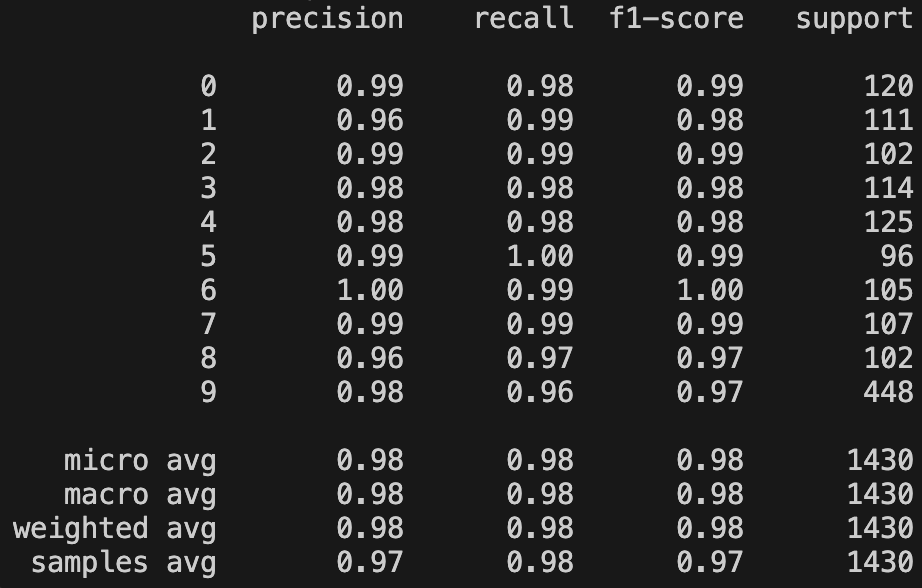
\includegraphics[width=0.7\textwidth]{Report_MLP.png}
%     \caption{ معیارهای ارزیابی برای تشخیص علائم دست در مدل شبکه چند لایه‌ای پرسپترونی}
% \end{figure}

\begin{figure}[h]
    \centering
    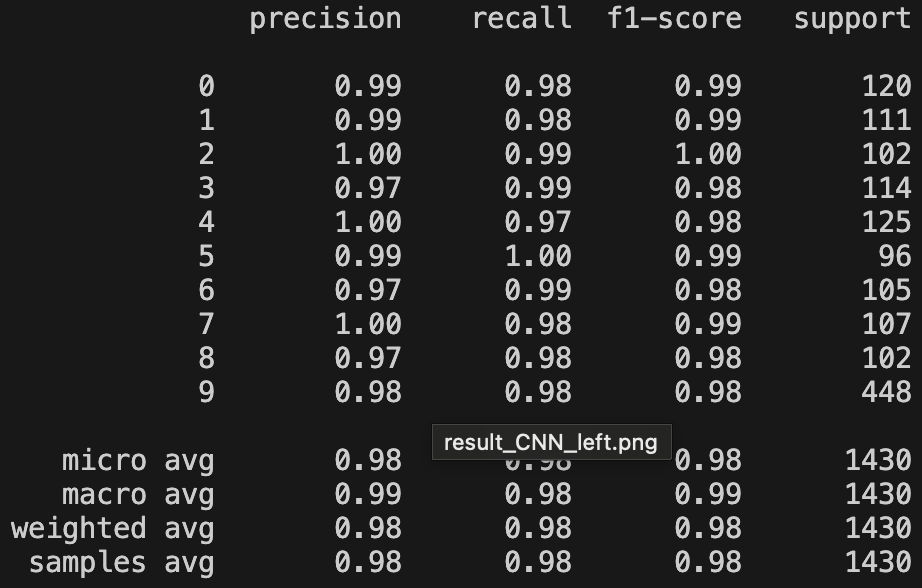
\includegraphics[width=0.7\textwidth]{Report_CNN.png}
    \caption{ معیارهای ارزیابی برای تشخیص علائم دست در مدل شبکه عصبی پیچشی}
    \label{report}
\end{figure}

% \begin{figure}[h]
%     \centering
%     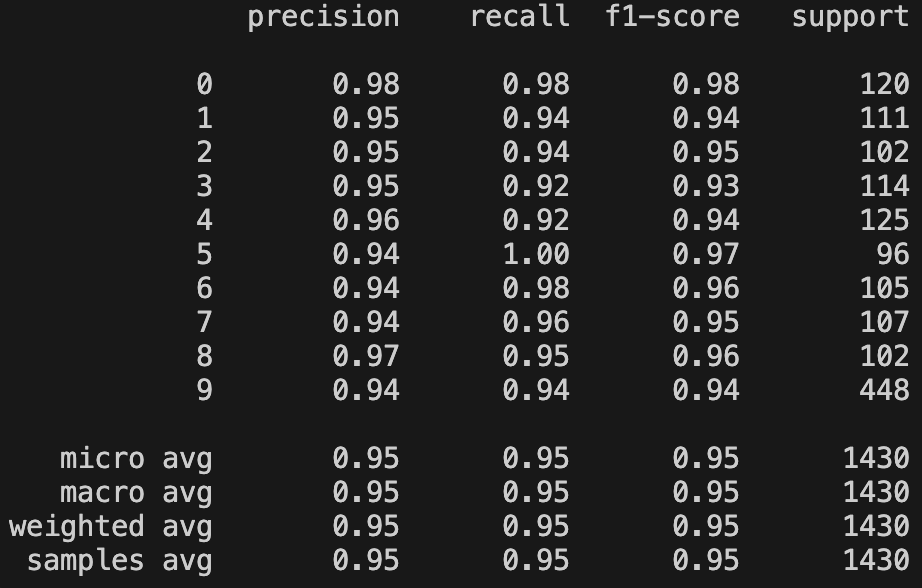
\includegraphics[width=0.7\textwidth]{Report_LSTM.png}
%     \caption{ معیارهای ارزیابی برای تشخیص علائم دست در مدل شبکه حافظه طولاني كوتاه مدت}
% \end{figure}

% \begin{figure}[h]
%     \centering
%     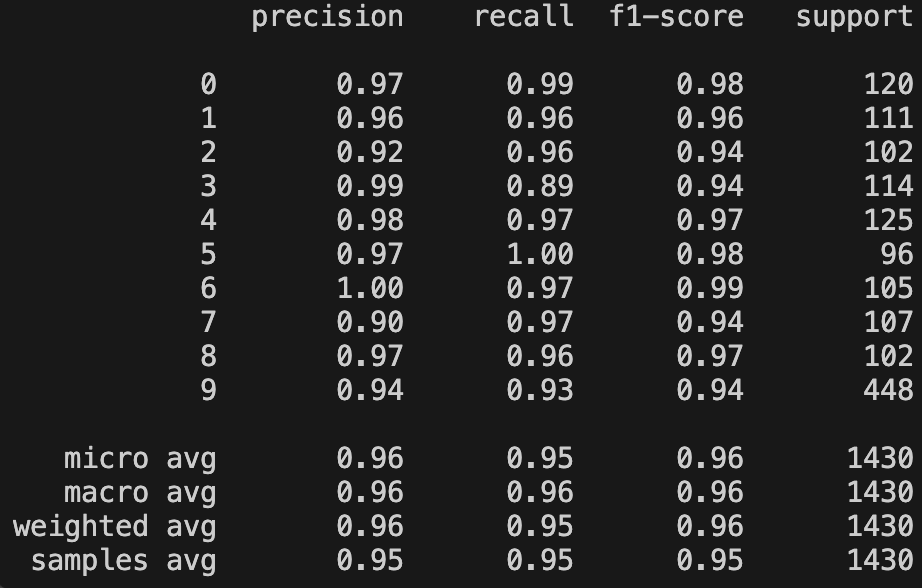
\includegraphics[width=0.7\textwidth]{Report_RNN.png}
%     \caption{ معیارهای ارزیابی برای تشخیص علائم دست در مدل شبکه عصبي بازگشتي}
% \end{figure}

\subsection[ماتریس درهم‌ریختگی]{ماتریس درهم‌ریختگی\protect\LTRfootnote{Confusion Matrix}}
ماتریس درهم‌ریختگی یک ابزار مهم در ارزیابی عملکرد مدل‌های طبقه‌بندی است. این ماتریس نشان‌دهنده تعداد نمونه‌هایی است که به درستی به هر کلاس تخصیص یافته‌اند و همچنین تعداد نمونه‌هایی که به اشتباه به کلاس‌های دیگر تخصیص داده شده‌اند. به عبارت دیگر، هر سطر این ماتریس نشان‌دهنده کلاس واقعی است و هر ستون نشان‌دهنده کلاسی است که مدل پیش‌بینی کرده است. اگر خانه \lr{ij} این ماتریس، عدد \lr{n} را داشته باشد، این به این معنا است که مدل \lr{n} بار نمونه‌های کلاس \lr{i} را به درستی به کلاس \lr{j} تخصیص داده است.
\\
ماتریس درهم‌ریختگی حاوی اطلاعات مفیدی است زیرا به ما اطلاعات دقیقی از عملکرد مدل در هر کلاس را می‌دهد. از این اطلاعات می‌توان برای ارزیابی عملکرد کلی مدل، شناسایی نقاط ضعف و قوت مدل، و بهبود آن استفاده کرد. همچنین، این ماتریس به ما امکان می‌دهد بررسی کنیم که آیا مدل ما به نسبت هر کلاس اشتباه می‌کند یا اشتباهات آن به کلاس‌های خاصی متمرکز شده‌اند \cite{Confusio72:online}.
ماتریس درهم ریختگی برای شبکه عصبی پیچشی که شبکه نهایی انتخاب شده  است در شکل \ref{matrix} آمده‌است.

% \begin{figure}[h]
%     \centering
%     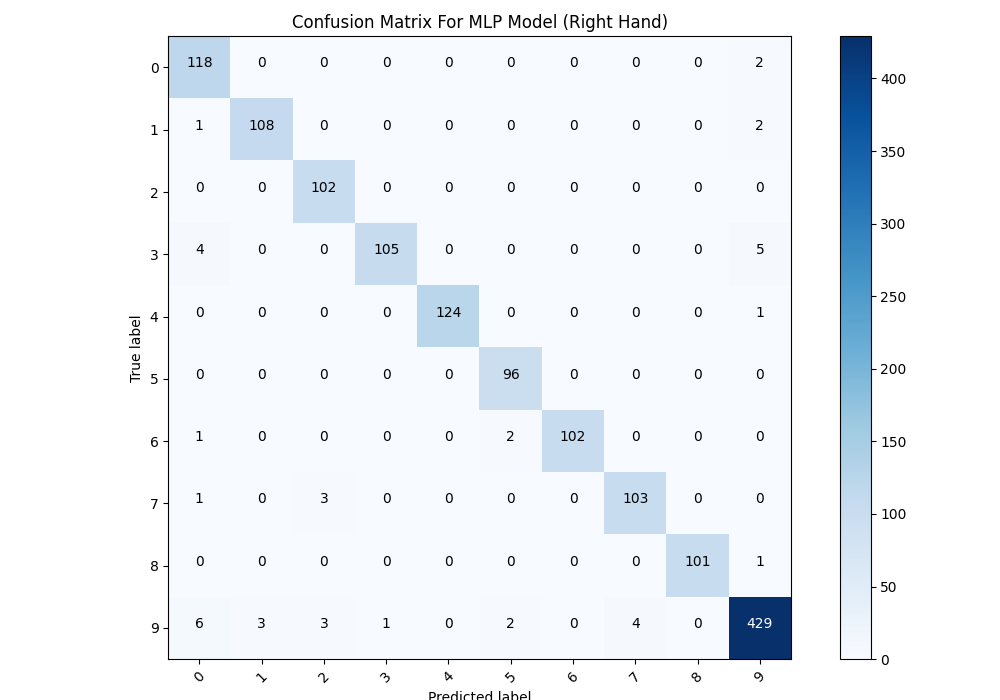
\includegraphics[width=0.8\textwidth]{Matrix_MLP_right.png}
%     \caption{ماتریس درهم‌ریختگی در مدل شبکه عصبی چندلایه‌ای پرسپترونی}
% \end{figure}


\begin{figure}[h]
    \centering
    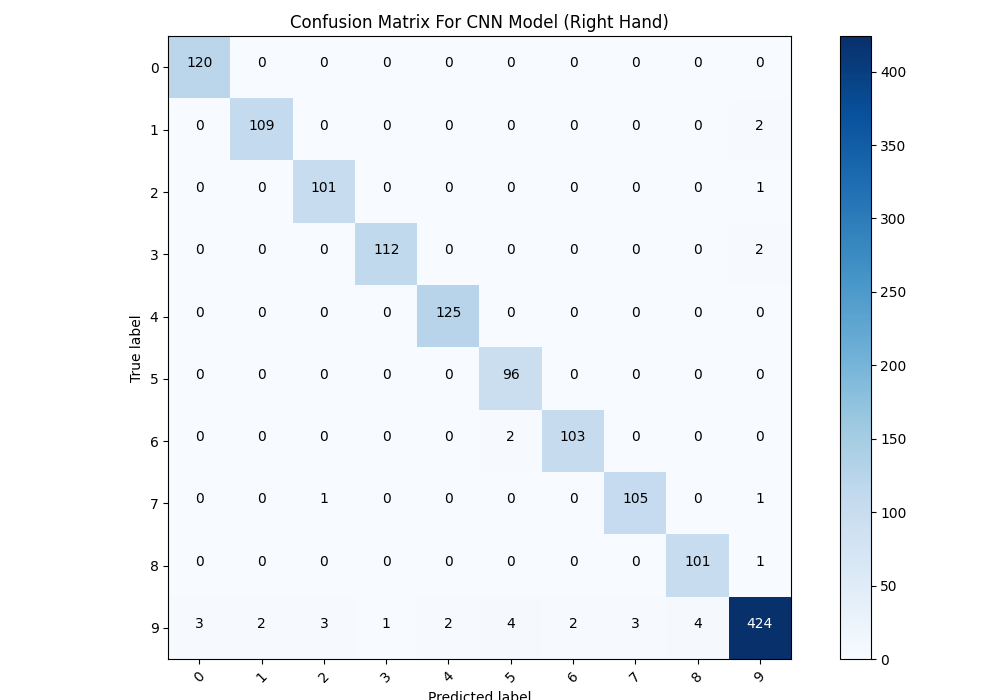
\includegraphics[width=0.8\textwidth]{Matrix_CNN_right.png}
    \caption{ ماتریس درهم‌ریختگی در مدل شبکه عصبی پیچشی}
    \label{matrix}
\end{figure}


% \begin{figure}[h]
%     \centering
%     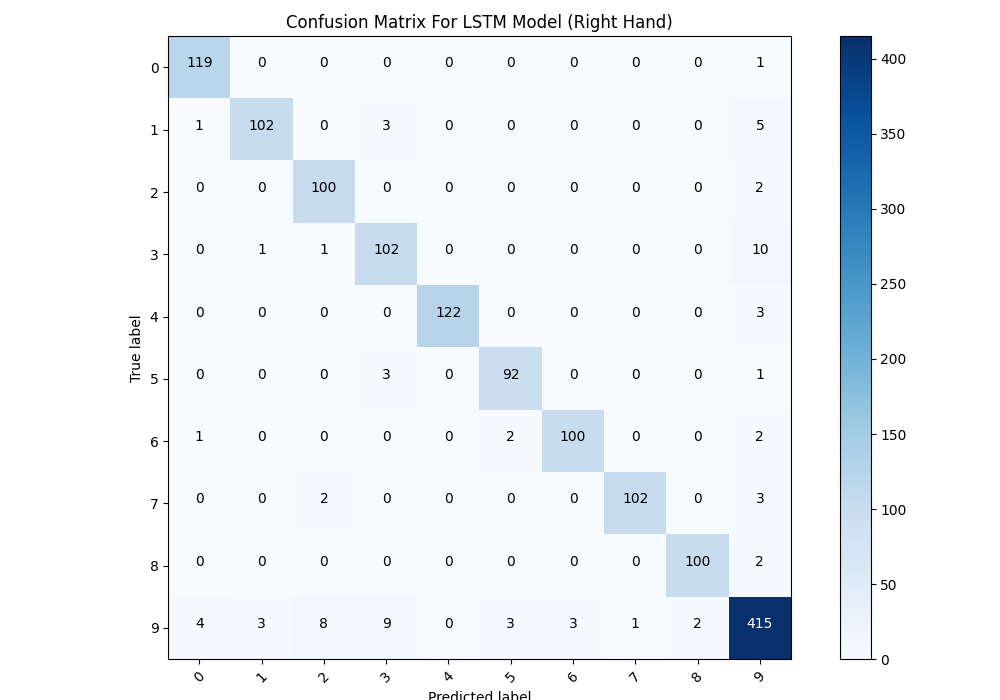
\includegraphics[width=0.8\textwidth]{Matrix_LSTM_right.png}
%     \caption{ ماتریس درهم‌ریختگی در مدل شبكه حافظه طولاني كوتاه مدت}
% \end{figure}


% \begin{figure}[h]
%     \centering
%     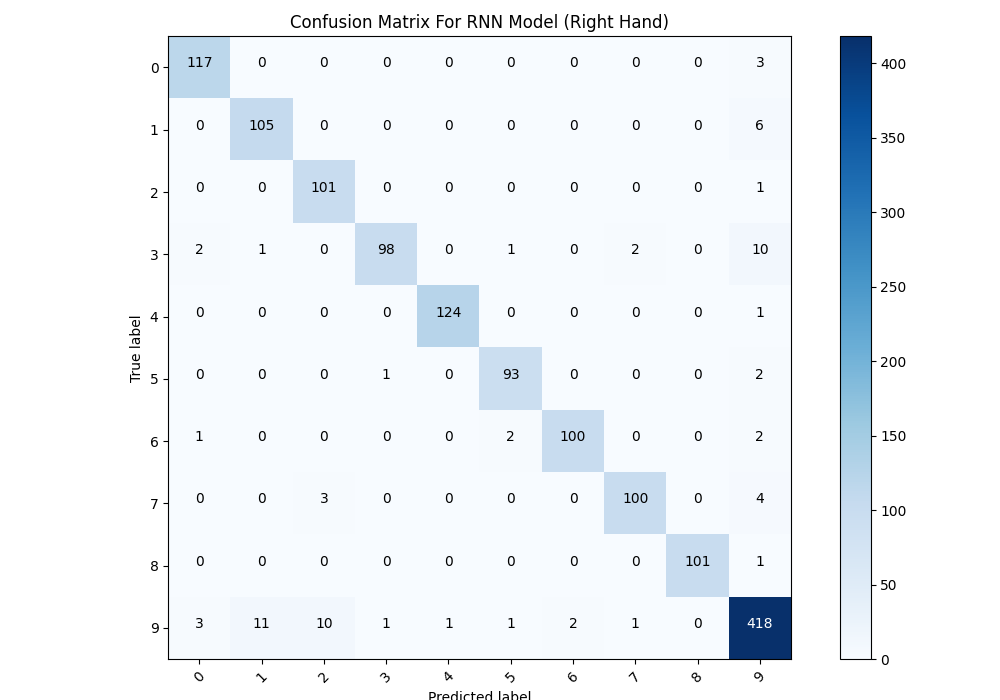
\includegraphics[width=0.8\textwidth]{matrix_RNN_right.png}
%     \caption{ ماتریس درهم‌ریختگی در مدل شبکه عصبي بازگشتي}
% \end{figure}


\section[نمودار‌های دقت و خطا بر حسب دوره]{ نمودار‌های دقت و خطا بر حسب دوره \LTRfootnote{Epoch}}
یک دوره زمانی است که کل مجموعه داده تنها یک بار از طریق شبکه عصبی انتشار پیدا کرده و پس از آن پس انتشار اتفاق می‌افتد
. از آنجایی که یک دوره ممکن است بسیار بزرگ باشد و نتوان آن را به یکباره به سیستم وارد کرد، به چند دسته کوچکتر تحت عنوان "دسته\LTRfootnote{Batch}" تقسیم می‌شود. انتقال کل مجموعه داده از طریق یک شبکه عصبی به تنهایی کافی نیست و باید مجموعه داده را چندین بار به شبکه ارسال کرد. در این پروژه، از یک مجموعه داده محدود استفاده شده و برای بهینه‌سازی یادگیری آن از الگوریتم گرادیان نزولی استفاده می‌کنیم.
\\
تعیین تعداد صحیح دوره‌ها از اهمیت بالایی برخوردار است. با افزایش تعداد دوره‌ها،‌ تعداد دفعات تغییر وزن در شبکه عصبی بیشتر می‌شود و منحنی یادگیری از حالت کم‌برازش\LTRfootnote{Underfitting} به حالت بهینه\LTRfootnote{Optimal} و در نهایت به حالت بیش‌برازش\LTRfootnote{Overfitting} تغییر می‌یابد. تعداد دوره‌ها باید به گونه‌ای تعیین شود که تعادلی برقرار شود و بتوان منحنی یادگیری را به بهترین حالت ممکن رساند.\\



\begin{figure}[h]
    \centering
    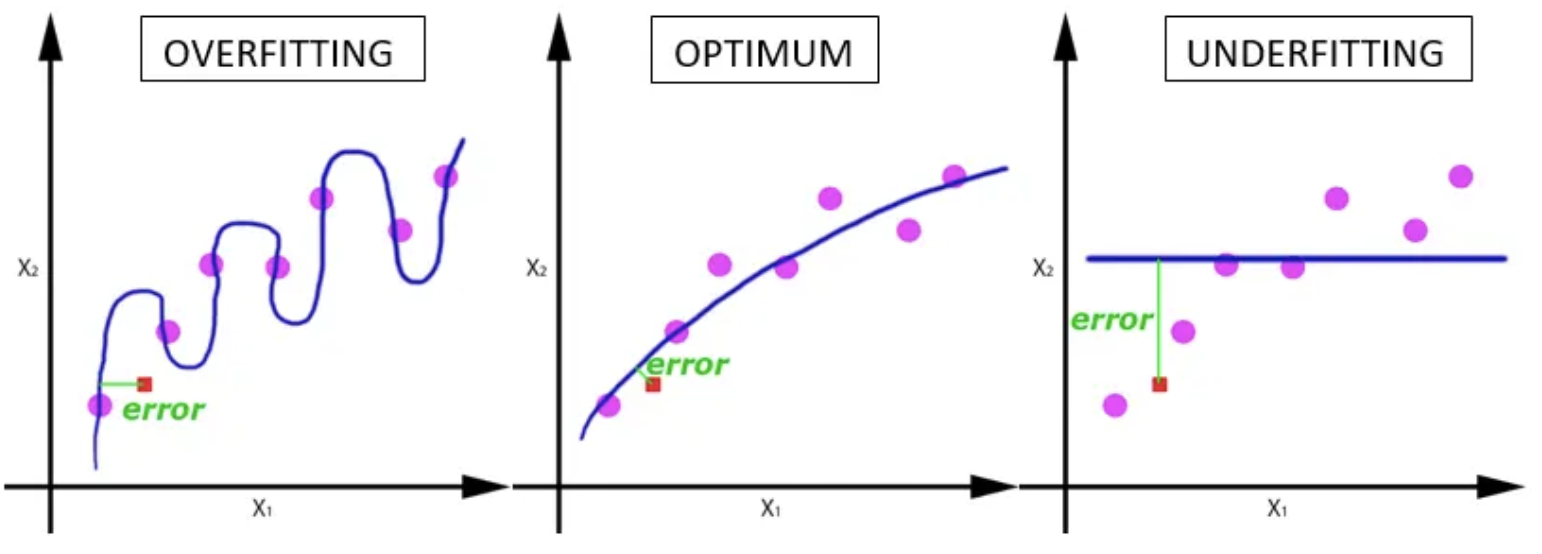
\includegraphics[width=1\textwidth]{fitting.png}
    \caption[منحنی‌ حالت‌های کم‌برازش، بهینه و بیش‌برازش]{منحنی‌ حالت‌های کم‌برازش، بهینه و بیش‌برازش \cite{wwwreddi92:online}}
\end{figure}


در این پروژه، به منظور نظارت و ارزیابی عملکرد مدل، نمودارهای دقت و خطا بر حسب دوره ترسیم شده‌اند, که در شکل \ref{acc} نمودار شبکه عصبی پیچشی آمده‌ است. این نمودارها نشان می‌دهند که چگونه دقت مدل و میزان خطا در طول زمان تغییر می‌کنند. بررسی این نمودارها می‌تواند به شناسایی نقاط بهینه و جلوگیری از بیش‌برازش کمک کند.




% \begin{figure}[h]
%     \centering
%     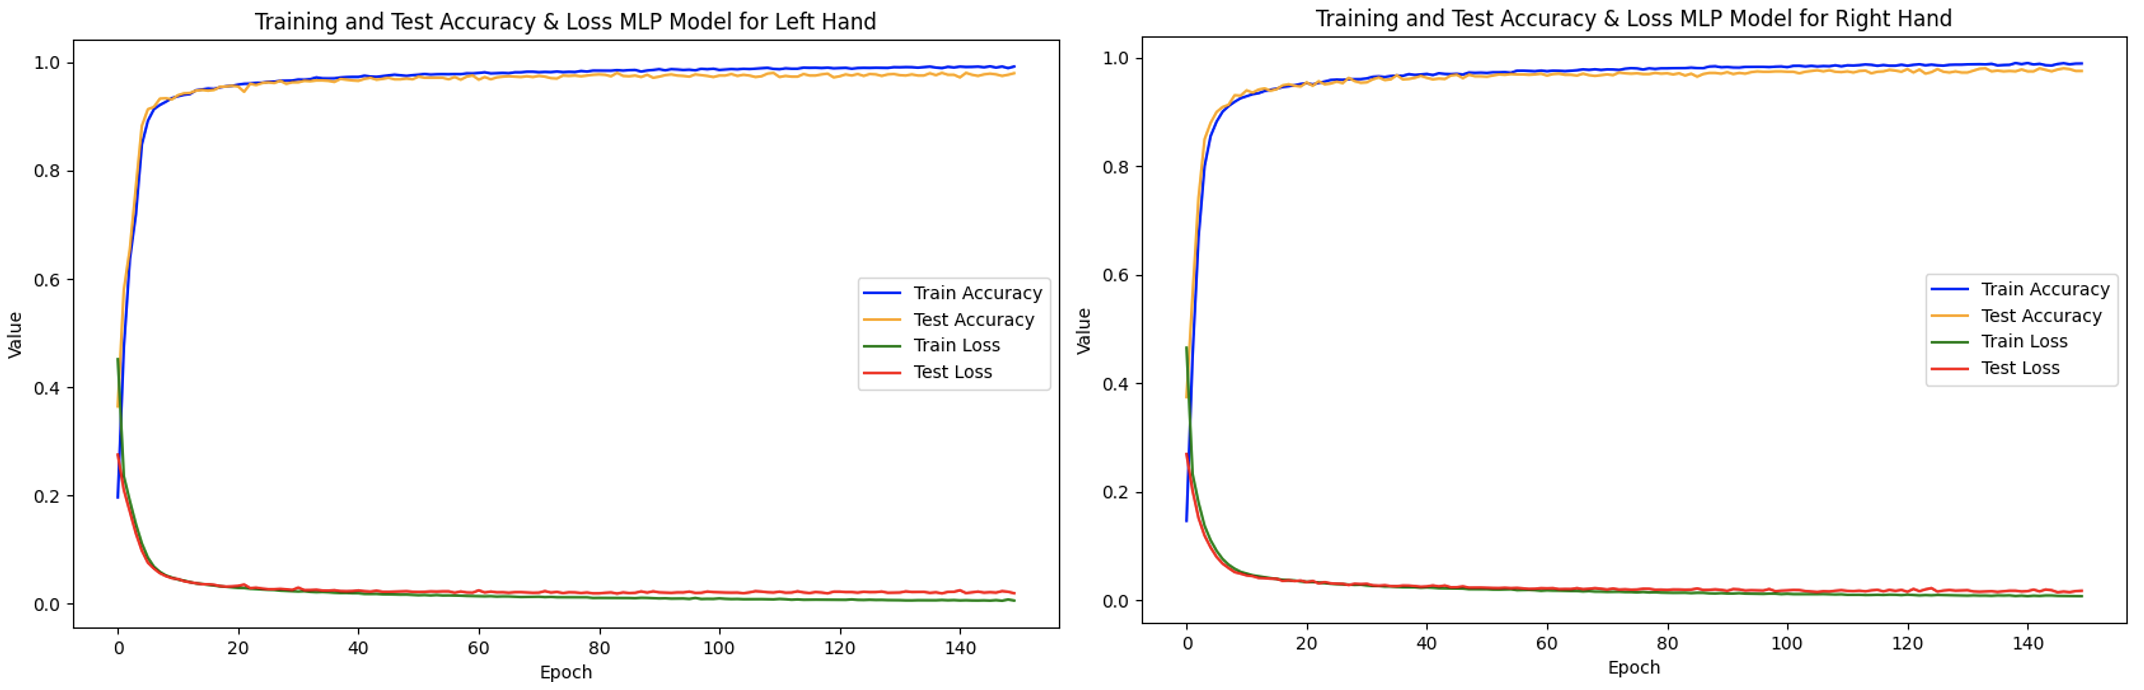
\includegraphics[width=1\textwidth]{Chart_MLP.png}
%     \caption{نمودار روند دقت و خطا در دست‌های راست و چپ بر حسب دوره در داده‌های آموزش و تست در مدل شبكه عصبي چندلايه پرسپتروني}
% \end{figure}

\begin{figure}[h]
    \centering
    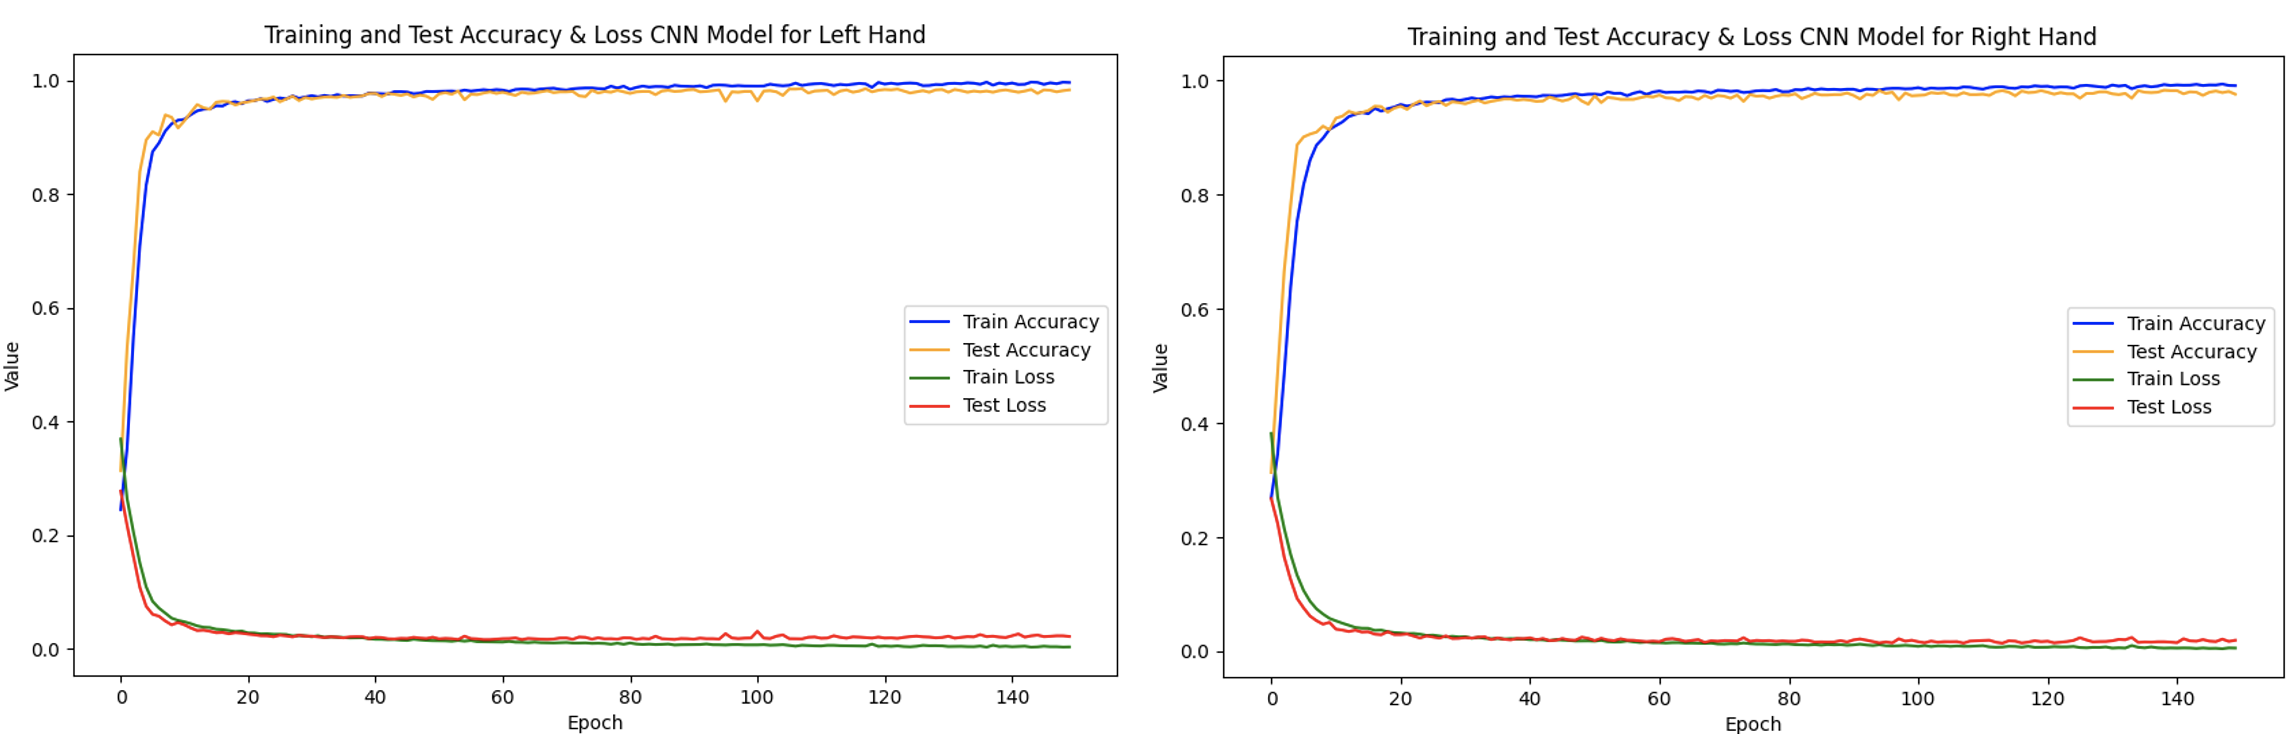
\includegraphics[width=1\textwidth]{Chart_CNN.png}
    \caption{نمودار روند دقت و خطا در دست‌های راست و چپ بر حسب دوره در داده‌های آموزش و تست در مدل شبکه عصبی پیچشی}
    \label{acc}
\end{figure}

% \begin{figure}[h]
%     \centering
%     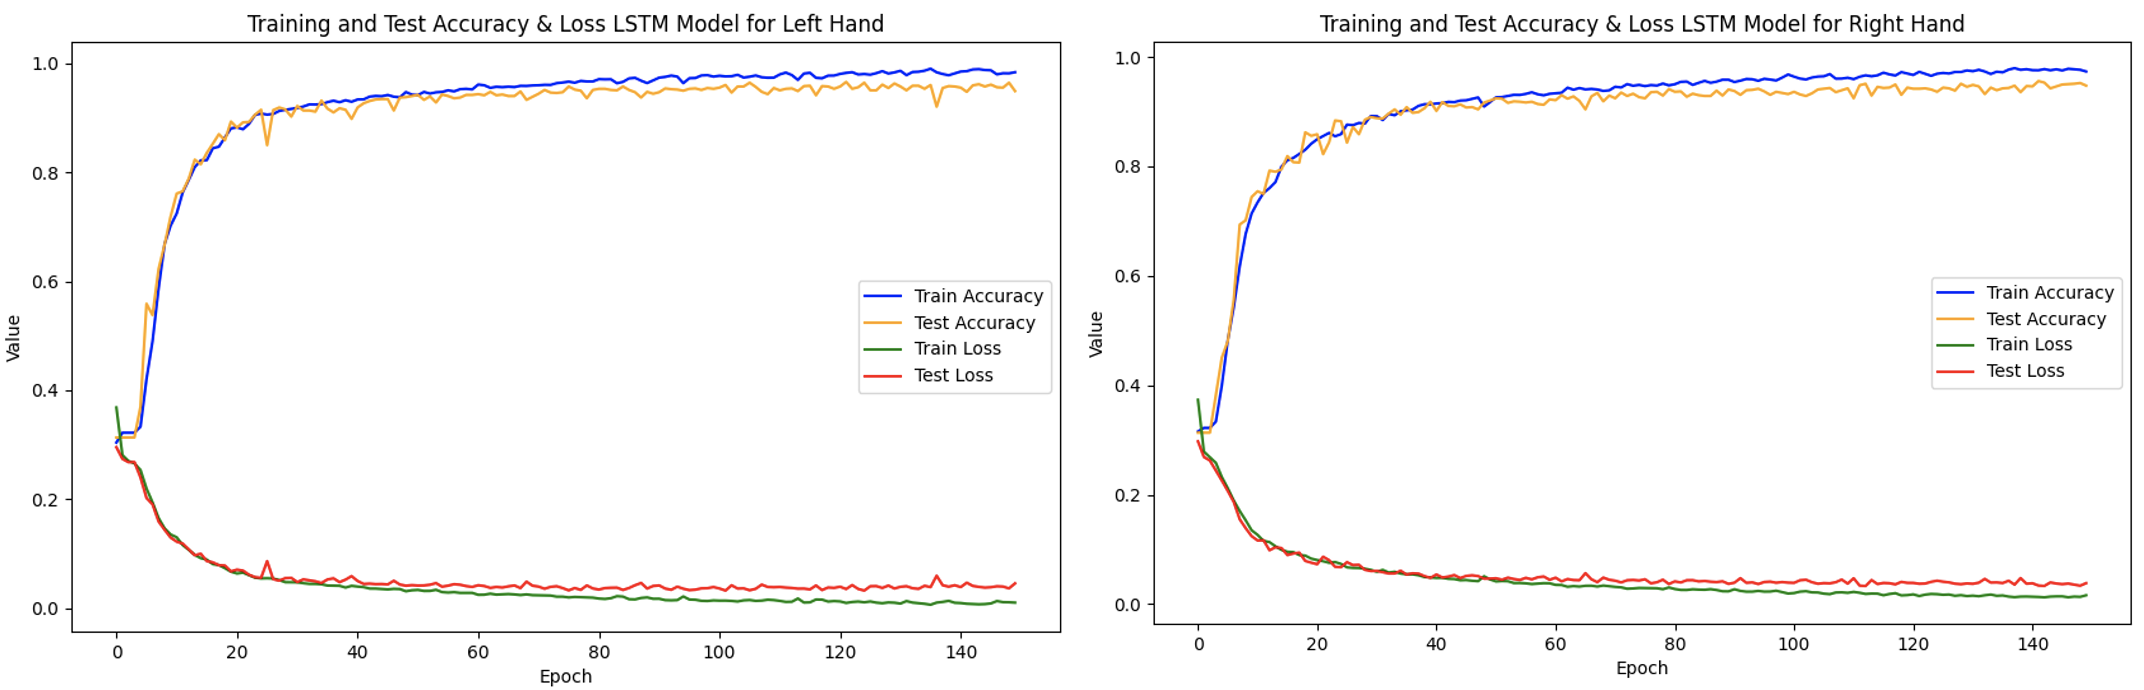
\includegraphics[width=1\textwidth]{Chart_LSTM.png}
%     \caption{نمودار روند دقت و خطا در دست‌های راست و چپ بر حسب دوره در داده‌های آموزش و تست در مدل شبكه حافظه طولاني كوتاه مدت}
% \end{figure}

% \begin{figure}[h]
%     \centering
%     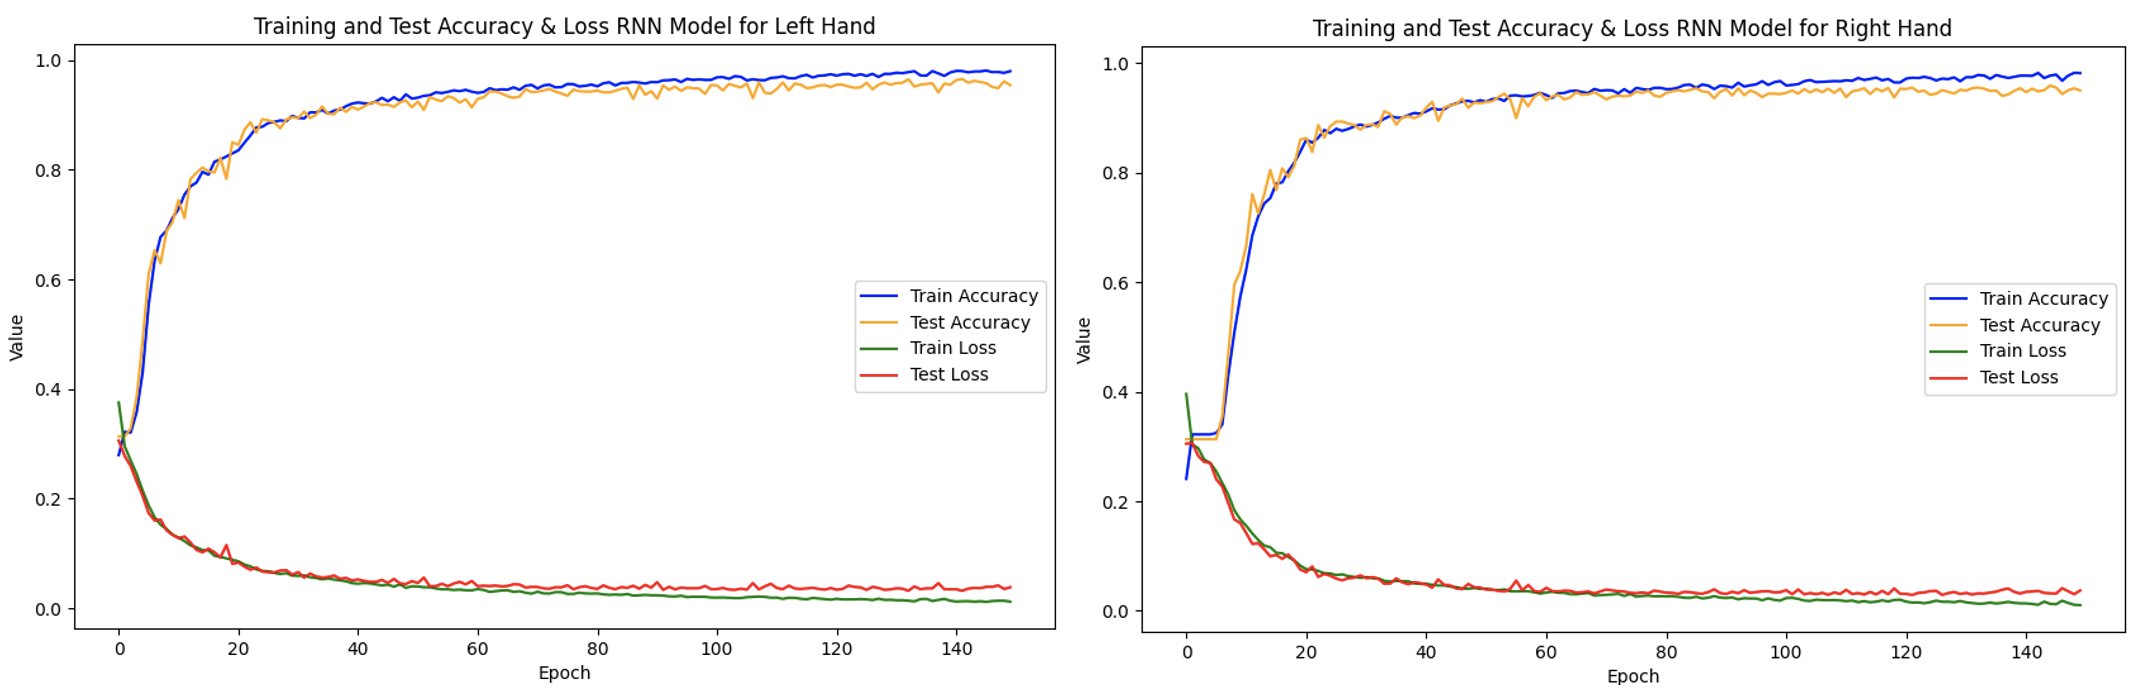
\includegraphics[width=1\textwidth]{Chart_RNN.png}
%     \caption{نمودار روند دقت و خطا در دست‌های راست و چپ بر حسب دوره در داده‌های آموزش و تست در مدل شبكه عصبي بازگشتي}
% \end{figure}


\section{تاثیر پس‌پردازش رأی‌گیری پنجره‌ای بر دقت}
به طور کلی با توجه به 
\cref{table:window}
 دقت ما پس از پیاده‌سازی رأی‌گیری پنجره‌ای کاهش پیدا کرده است. اما لزوم این الگوریتم برای ما از اهمیت ویژه‌ای برخوردار است, چرا که در بیشتر مواردی که دقت به درستی بیان نشده است در زمانی است که علائم دست کاربر نمادی را نشان داده اما پهپاد از آن پیروی نمی‌کند. این موضوع می‌تواند سبب ناخوشایندی کاربر شود، اما این الگوریتم سبب شده است تا بسیاری از
 مواردی که علائم دست در یک یا تعداد کمی از فریم‌ها توسط سیستم اشتباه برداشت شده‌است، یا حتی کاربر در مدت کوتاهی به اشتباه هدف خود را بیان کند، دستور نهایی صادر نشود تا پهپاد دچار مشکل نشود.

\begin{table}[h!]
    \centering
    \begin{tabular}{||>{\centering\arraybackslash}p{5.5cm} >{\centering\arraybackslash}p{4cm} >{\centering\arraybackslash}p{4cm}||}
     \hline
     \rule{0pt}{3ex} معماری مدل & دقت مدل بدون رأی‌گیری پنجره‌ای & دقت مدل با رأی‌گیری پنجره‌ای \\ [1.5ex]
     \hline
     \hline
     \rule{0pt}{0.5ex} & & \\  
     شبکه عصبی چندلایه‌ای پرسپترونی & ۶۷.۹۷ \text{\%} & ۳۷.۹۸ \text{\%}\\ [2.5ex]
     شبکه عصبی پیچشی & ۲۷.۹۸ \text{\%} & ۹۸.۹۸ \text{\%} \\ [2.5ex]
     شبکه عصبی حافظه طولانی کوتاه مدت & ۲۴.۹۵ \text{\%} & ۹۲.۹۵ \text{\%} \\ [2.5ex]
     شبکه عصبی بازگشتي & ۰۲.۹۵ \text{\%} & ۷۰.۹۵ \text{\%} \\ [2.5ex]
     \hline
    \end{tabular}
    \caption{جدول ارزیابی تاثیر رأی‌گیری پنجره‌ای در دقت  با استفاده از یک ویدیو دوازده هزار فریمی}
    \centering
    \label{table:window}
\end{table}


\section{سرعت اجرای برنامه}
به منظور رسیدن به یکی از اهداف اصلی این پروژه، که بی‌درنگ بودن آن می‌باشد، لازم است که میزان پاسخ‌گویی مدل‌ها نیز مورد بررسی و ارزیابی قرار گیرد. در 
\cref{table:1}
زمان پاسخ‌گویی مدل‌ها از زمانی که داده‌ها از طریق دوربین خوانده می‌شوند تا زمانی که دستور به پهپاد داده می‌شود، آورده شده است.

\begin{table}[h!]
    \centering
    \begin{tabular}{||c c||}
     \hline
     \rule{0pt}{3ex}معماری مدل & زمان پاسخگویی مدل\\ [1.5ex]
     \hline
     \hline
     \rule{0pt}{0.5ex} & \\  % Adds space before the first data row, while keeping the vertical lines
     شبکه چندلایه‌ای پرسپترونی & 4 $\pm$ 39 میلی‌ثانیه \\ [2.5ex]
     شبکه عصبی پیچشی & 7 $\pm$ 41 میلی‌ثانیه  \\ [2.5ex]
     شبکه عصبی  حافظه طولانی کوتاه مدت & 1 $\pm$ 44 میلی‌ثانیه  \\ [2.5ex]
     شبكه عصبي بازگشتي & 2 $\pm$ 41 میلی‌ثانیه  \\ [2.5ex]

     \hline
    \end{tabular}
    \caption{جدول ارزیابی زمان پاسخگویی مدل‌ها}
    \label{table:1}
\end{table}


\section{سخت‌افزار مورد نیاز}
این پروژه باید به گونه‌ای اجرا می‌شد که بر روی ساده‌ترین سیستم‌های کامپیوتری نیز قابل اجرا باشد، زیرا سخت‌افزار پهپادها به‌طور معمول دارای پردازنده‌ و و حافظه‌های موقت 
\LTRfootnote{Ram}
ضعیف‌تری هستند. همچنین، استفاده از پردازنده گرافیکی ممکن نبود، چرا که پهپادها فاقد پردازنده‌های گرافیکی می‌باشند. 
معماری‌های پیاده‌سازی شده به نحوی طراحی شدند که تعادل میان دقت و بهره‌وری از سخت‌افزار حفظ شود، به طوری که هم قابلیت اجرا به صورت بی‌درنگ را داشته باشند و هم امکان پیاده‌سازی آن‌ها بر روی پهپاد فراهم باشد. از این رو، معماری‌ها به گونه‌ای پیاده‌سازی شدند که بر روی پردازنده‌های سبک با میزان حافظه موقت کم اجرا شوند.
میزان استفاده از حافظه موقت برای اجرای معماری‌های پیاده‌سازی شده در این پروژه به شرح زیر است:



\begin{table}[h!]
    \centering
    \begin{tabular}{||c c c||}
     \hline
     \rule{0pt}{3ex}معماری مدل & حجم مدل & حافظه موقت مورد نیاز برای اجرا \\ [1.5ex]
     \hline
     \hline
     \rule{0pt}{0.5ex} & & \\  % Adds space before the first data row, while keeping the vertical lines
     شبکه چندلایه‌ای پرسپترونی & ۱۰۹ کیلوبایت & ۹۹۲.۹ کیلوبایت \\ [2.5ex]
     شبکه عصبی پیچشی & ۲۷۰ کیلوبایت & ۹۵۳.۱۰ کیلوبایت \\ [2.5ex]
     شبکه عصبی  حافظه طولانی کوتاه مدت & ۶۲۷ کیلوبایت & ۹۷۴.۱۳ کیلوبایت \\ [2.5ex]
     شبکه عصبی بازگشتي & ۴۰۱ کیلوبایت & ۱۵۸.۱۳ کیلوبایت \\ [2.5ex]
     \hline
    \end{tabular}
    \caption{جدول ارزیابی حافظه موفت موردنیاز مدل‌ها}
    \label{table:4}
\end{table}

\section{مقایسه دقت پروژه با کارهای مشابه}
پروژه پیاده‌سازی از دقت بسیار بالایی برخوردار است که این دقت به دلیل ترکیب پیش‌پردازش، کتابخانه مدیاپایپ، مدل کلاس‌بندی و پس‌پردازش است. 
\\ در این قسمت به مقایسه دقت پروژه پیاده‌سازی شده با پروژه‌های مشابه با هدف کنترل پهپاد با کمک تشخیص علائم دست پرداخته‌ایم.

\begin{table}[h!]
    \centering
    \begin{tabular}{||>{\centering\arraybackslash}p{10.5cm} >{\centering\arraybackslash}p{2cm} >{\centering\arraybackslash}p{2cm}||}
     \hline
     \rule{0pt}{3ex} نام مقاله & تعداد علائم‌ دست & دقت تشخیص علائم دست \\ [1.5ex]
     \hline
     \rule{0pt}{0.5ex} & & \\  
     برنامه ما & 9 & 32.98 \text{\%} \\ [2.5ex]
     پهپادهاي كنترل شده با علائم دست به صورت متن باز \cite{natarajan2018hand} & 5 & ۴۷۱.۹۷ \\ [2.5ex]
     روشهاي تشخيص علائم دست به صورت بي‌درنگ \cite{fang2007real} & 6 & 8.93 \text{\%} \\ [2.5ex]
     تشخيص علائم دست براي كنترل پهپاد با استفاده از ياديگيري عميق \cite{hadri2018hand} & 9 & 3.83 \text{\%} \\ [2.5ex]
     علائم يوايوي: مجموع‌داده براي يوايوي كنترل و تشخيص علائم \cite{perera2018uav} & 13 & 9.91 \text{\%} \\ [2.5ex]
     تشخيص علائم دست براي استفاده‌هاي بي‌درنگ \cite{murugeswari2014hand} & 6 & 8.90 \text{\%} \\ [2.5ex]
     روشي بهبود يافته براي تشخيص علائم دست با استفاده از نقاط كليدي و جعبه مرزي \cite{dang2022improved} & 6 & 94 \text{\%} \\ [2.5ex]
     تشخیص حرکت دست با استفاده از تکنیک های بینایی ماشین \cite{rios2013hand} & 6 & 1.93 \text{\%} \\ [2.5ex]
     تشخیص علائم دست با استفاده از تکنیک‌های پردازش تصویر و استخراج ویژگی \cite{sharma2020hand} & 28 & 54.89 \text{\%} \\ [2.5ex]
     استفاده از تشخیص حرکت دست برای برنامه راهنمای کاربر با استفاده از مدیاپایپ \cite{harris2021applying} & 10 & 95 \text{\%} \\ [2.5ex]
     دست‌هاي مدياپايپ: تشخيص بي درنگ دست بر روي دستگاه‌ها \cite{zhang2020mediapipe} & 8 & 7.94 \text{\%} \\ [2.5ex]
     سیستم تشخیص حرکت دست مبتنی بر بینایی کامپیوتر و یادگیری ماشین \cite{trigueiros2015hand} & 28 & 72.93 \text{\%} \\ [2.5ex]
     تشخیص علائم دست با استفاده از مدل های پنهان مارکوف \cite{min1997hand} & 5 & 1.92 \text{\%} \\ [2.5ex]
     تشخیص علائم دست با استفاده از کینکت \cite{li2012hand} & 38 & 84 \text{\%} \\ [2.5ex]
     تشخیص علائم دست با استفاده از شبکه های عصبی \cite{murthy2010hand} & 10 & 89 \text{\%} \\ [2.5ex]
     \hline
    \end{tabular}
    \caption{جدول مقایسه پروژه با کارهای مشابه}
\end{table}

\pagebreak


\section{جمع‌بندی}
مدل‌های ارائه شده در این پروژه دارای دقت و کارایی مناسبی هستند که امکان استفاده آن‌ها در کاربردهای واقعی را فراهم می‌کند. این مدل‌ها قادرند به خوبی علائم‌ دست را تشخیص داده و از آن‌ها در عملیات مختلفی مانند کنترل دستگاه‌ها و رابط‌های کاربری استفاده کنند.
\\
علاوه بر این، با مقایسه عملکرد  این پروژه با کارهای مشابه در حوزه تشخیص علائم‌ دست، مشخص شده است که پروژه‌ی ما دارای دقت مشابه یا حتی بالاتری است، به ویژه اگر تعداد کلاس‌های علائم دست در نظر گرفته شود. این نکته نشان می‌دهد که مدل‌های ارائه شده به خوبی تنوع و پیچیدگی علائم‌ دست را درک می‌کنند و قادر به تشخیص آن‌ها هستند، که این امر یکی از چالش‌های اصلی در این زمینه است.
\\
با توجه به این نتایج، می‌توانیم اطمینان داشته باشیم که پروژه‌ی ما قادر است به عنوان یک راه‌حل کارآمد برای تشخیص علائم‌ دست در برنامه‌ها و سیستم‌های واقعی مورد استفاده قرار بگیرد.
در فصل بعدی به جمع‌بندی کلی این پروژه و ارائه پیشنهاداتی برای بهبود عملکرد سیستم طراحی شده می‌پردازیم.


% \chapter{نتیجه گیری و پیشنهادات}
% \section{مقدمه}
% در این فصل، ما به بررسی نتایج بدست آمده و ارائه پیشنهاداتی می‌پردازیم که می‌توانند عملکرد سیستم کنترل پهپاد را از جنبه‌های مختلف بهبود بخشند. 
% نتایج به‌دست‌آمده در این پروژه نشان‌دهنده دقت بالای سیستم در تشخیص علائم‌ها و انتقال دستورات به پهپاد می‌باشد. با این حال، همچنان می‌توان بهبودهایی در عملکرد سیستم اعمال کرد تا دقت و کارایی آن افزایش یابد.
% این پیشنهادات شامل افزایش سرعت اجرای برنامه، بهبود دقت پیش‌بینی علائم‌ها و کاهش محدودیت‌های منابع 
% می‌باشند. هدف از این فصل، ارائه راهکارهای عملی و کاربردی است که بتوانند سیستم را به سطح بالاتری از کارایی و اطمینان برسانند.
\section{مقدمه}
در این فصل، ما به بررسی نتایج بدست آمده از این پروژه و ارائه پیشنهاداتی می‌پردازیم که می‌توانند عملکرد سیستم کنترل پهپاد را از جنبه‌های مختلف بهبود بخشند. نتایج به‌دست‌آمده در این پروژه نشان‌دهنده دقت بالای سیستم در تشخیص علائم و انتقال دستورات به پهپاد می‌باشد. با این حال، همچنان می‌توان بهبودهایی در عملکرد سیستم اعمال کرد تا دقت و کارایی آن افزایش یابد.
\\
این پیشنهادات شامل افزایش سرعت اجرای برنامه، بهبود دقت پیش‌بینی علائم و کاهش محدودیت‌های منابع می‌باشند. هدف از این فصل، ارائه راهکارهای عملی و کاربردی است که بتوانند سیستم را به سطح بالاتری از کارایی و اطمینان برسانند.


\section{نتیجه‌گیری}
نتایج به‌دست‌آمده در این پروژه نشان‌دهنده عملکرد دقیق و موفقیت‌آمیز آن است. این پروژه به تمامی اهداف از پیش تعیین‌شده، از جمله دقت بالا، صحت قابل قبول، فراخوانی مناسب، امتیاز \lr{F1} بالا، اجرای بی‌درنگ، رضایت کاربر، خطای پایین و قابلیت پیاده‌سازی بر روی پهپاد دست یافته است. عملکرد دقیق سیستم در تشخیص و کنترل پهپاد با استفاده از علائم دست، نشان‌دهنده پتانسیل بالای این روش برای کاربردهای مختلف در صنعت و تکنولوژی است.


\section{پیشنهادات}
در این بخش پیشنهاداتی برای بهبود عملکرد پهپاد با کنترل دست بیان شده‌است.
\subsection{محدودیت وجود پهپاد‌های منبع‌باز}
در مورد محدودیت‌های استفاده از پهپادهای منبع‌باز و شرکتی برای پروژه کنترل پهپاد با استفاده از علائم دست بر مبنای بینایی ماشین، چندین موضوع موردنظر وجود دارد. 
\\
ابتدا، در مورد پهپادهای شرکتی، باید توجه داشت که این پهپادها معمولاً دارای سیستم‌های بسته و غیرقابل تغییر هستند که مانع از انجام تغییرات و سفارشی‌سازی‌های مورد نیاز برای اجرای الگوریتم‌های پیچیده بر روی آنها می‌شوند. همچنین، 
محدودیت‌های قانونی و مقرراتی مانند نیاز به مجوزهای خاص برای استفاده از پهپادهای تجاری در برخی کشورها می‌توانند چالش‌هایی را ایجاد کنند.
\\
در مورد پهپادهای منبع‌باز، محدودیت‌های متفاوتی وجود دارد. این پهپادها ممکن است دارای سخت‌افزارهای قدرتمندی نباشند که بتوانند الگوریتم‌های پیچیده پردازش تصویر را اجرا کنند. همچنین، عدم پشتیبانی کامل از زبان‌های برنامه‌نویسی مدرن می‌تواند باعث پیچیدگی در توسعه و اجرای برنامه‌ها شود.
\\
با در نظر گرفتن این محدودیت‌ها، راهکار ساخت یک پهپاد سفارشی با سخت‌افزار مناسب و قابلیت برنامه‌نویسی مورد نیاز، می‌تواند راه حلی مناسب باشد. این رویکرد امکان اجرای الگوریتم‌های پیچیده و پیاده‌سازی برنامه‌های سفارشی را فراهم می‌کند، که باعث بهبود کارایی و انعطاف‌پذیری سیستم در ارتباط با کنترل پهپاد با علائم دست خواهد شد.

\subsection{وجود چندین دست در تصویر}
وجود چندین دست در تصویر یک چالش بزرگ در برنامه است. در این مورد باید به این نکته توجه کنیم که در یک فریم تصویر، ممکن است چندین دست قابل مشاهده باشند که این می‌تواند برای الگوریتم‌های تشخیص دست مشکل‌ساز شود. زیرا 
الگوریتم‌ها باید بتوانند دست‌ها را تفکیک کرده و علائم متفاوت آنها را تشخیص دهند. همچنین ممکن است دست‌های غیرمرتبط با کاربر، مانند دست‌های در پس‌زمینه یا دست‌های دیگر افراد، نیز در تصویر حضور داشته باشند که این موضوع می‌تواند دقت الگوریتم را کاهش دهد.
\\
یکی از راهکارهای موردنظر برای حل این چالش، شخصی‌سازی مدل تشخیص دست با توجه به داده‌هایی که از کاربران جمع‌آوری می‌شود، است. این روش می‌تواند به کمک داده‌های جمع‌آوری شده از دست‌های واقعی کاربران، به مدل کمک 
کند تا الگوهای مختلف دست‌ها را بیشتر بشناسد و از این طریق دقت تشخیص را افزایش دهد. با این حال، این روش نیازمند زمان و تلاش برای جمع‌آوری و برچسب‌گذاری داده‌های موردنیاز است و ممکن است برای کاربران خوشایند نباشد.
\\
راهکار دیگری که می‌توان برای حل این مسئله در نظر گرفت، استفاده از یک سیستم ارتباطی میان دست و پهپاد است. به این ترتیب، کاربر می‌تواند یک دستبند یا سیمی را در دست خود داشته باشد که این دستبند به عنوان نشانه تشخیص دست و 
ارتباط بین کاربر و پهپاد عمل کند. با این روش، پهپاد تنها دستی را که دارای دستبند است شناسایی می‌کند و به دستورات آن پاسخ می‌دهد. این راهکار می‌تواند از دقت و سرعت الگوریتم تشخیص بهره‌مند شود و به کاربر اطمینان بیشتری بدهد. با 
این حال، برای اجرای این روش نیازمند توسعه و اعمال یک مدل دیگر برای تشخیص دست با دستبند است که این می‌تواند زمان و هزینه بیشتری را به بار آورد.


\subsection{شناسایی یک دست در دو مرتبه}
یکی از مشکلاتی که بسیاری از استفاده‌کنندگان کتابخانه مدیاپایپ با آن مواجه شده‌اند، مربوط به شناسایی یک دست در دو مستطیل متفاوت و در نتیجه دو خروجی است. این مشکل می‌تواند به علت همپوشانی بین دو مستطیلی که دست را 
شناسایی می‌کنند، ایجاد شود. با این حال، این مشکل برای پروژه خاصی که ما در دست داریم تفاوتی ایجاد نکرده است، زیرا ما یک گزینه را انتخاب کرده و علائم دست را در آن پیش‌بینی می‌کنیم.
\\
از بین بردن این مشکل می‌تواند بهبود و بهینه‌سازی کارایی این کتابخانه را برای سایر استفاده‌کنندگان افزایش دهد. برای حل این مشکل، می‌توان محدودیتی برای همپوشانی مستطیل‌های حاوی دست را در نظر گرفت. به این صورت که اگر دو مستطیل بیشتر از حد در نظر گرفته شده 
همپوشانی داشته باشند، یعنی یک دست در دو تصویر تشخیص داده شده باشد، تنها یکی از آنها به مدل بعدی ارسال شود.
\begin{figure}[h]
    \centering
    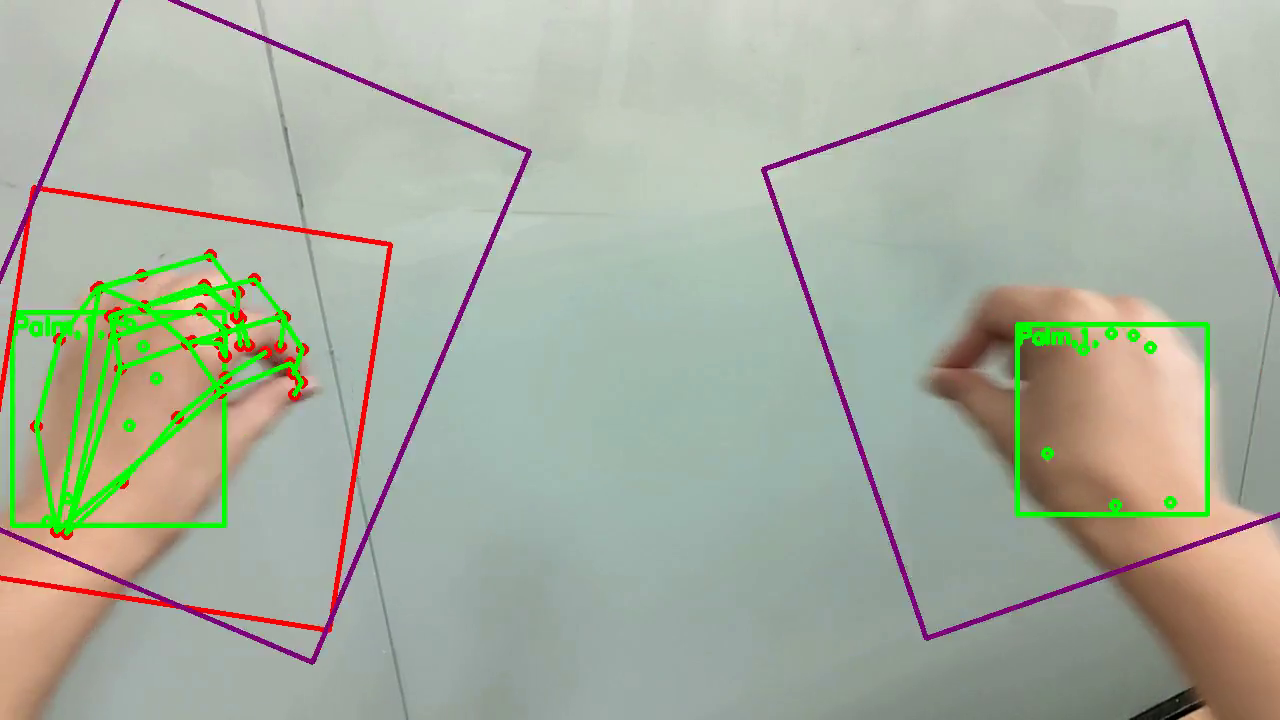
\includegraphics[width=0.6\textwidth]{multi_boxes.png}
    \caption{شناسایی یک دست دو مرتبه}
\end{figure}


\subsection{اجرا بر روی پردازنده‌های گرافیکی }
پروژه ما  به علت عدم دسترسی به پهپادی که از پردازنده‌های گرافیکی برای اجرای مدل‌ها استفاده می‌کند, به صورتی پیاده‌سازی شده است که تنها بر روی پردازنده مرکزی قابل اجرا است. با این حال، اگر پهپادی با توانایی اجرای مدل‌ها بر روی 
پردازنده‌های گرافیکی در دسترس باشد، سه مدل که به صورت پی‌در‌پی اجرا می‌شوند می‌توانند بر روی پردازنده‌های گرافیکی اجرا شده تا عملکرد سیستم را ارتقا داده و تجربه کاربری را بهبود بخشند. استفاده از پردازنده‌های گرافیکی برای اجرای مدل‌ها می‌تواند 
سرعت پردازش را بسیار افزایش دهد، زیرا کارت‌های گرافیکی معمولاً دارای تعداد زیادی هسته محاسباتی هستند که برای پردازش موازی و سریع داده‌ها بسیار مناسب هستند. این امر می‌تواند منجر به بهبود قابل توجهی در زمان پاسخ و دقت 
تشخیص علائم دست شود و تجربه کاربری را بهبود بخشد. به علاوه، با استفاده از پردازنده‌های گرافیکی، می‌توانیم بار محاسباتی را از پردازنده مرکزی کاهش داده و عملکرد کلی سیستم را بهتر کنیم.

\subsection{اجرای پروژه با برنامه سی پلاس پلاس}
با توجه به مزایای زبان سی پلاس پلاس نسبت به پایتون، انتخاب این زبان برای انجام این پروژه می‌تواند به بهبود عملکرد و کارایی سیستم کمک شایانی کند. در ادامه به برخی از مزایای استفاده از زبان سی پلاس پلاس نسبت به پایتون در این پروژه پرداخته شده است:

\begin{itemize}
    \item عملکرد و سرعت اجرای بالا: سی پلاس پلاس یک زبان برنامه‌نویسی کامپایل‌شده است که به کد ماشین تبدیل می‌شود، به همین دلیل عملکرد و سرعت اجرای بسیار بالاتری نسبت به پایتون دارد که یک زبان تفسیری است. این ویژگی
    برای پروژه‌های بی‌درنگ مانند کنترل پهپاد با استفاده از علائم دست بسیار حیاتی است، زیرا زمان پاسخ‌دهی سریع و دقیق در این سیستم‌ها اهمیت زیادی دارد.
    \item مدیریت دقیق حافظه: سی پلاس پلاس امکان مدیریت دقیق حافظه را فراهم می‌کند. این ویژگی می‌تواند بهینه‌سازی استفاده از منابع سیستم و کاهش مصرف حافظه را به دنبال داشته باشد، که برای سیستم‌هایی 
    با منابع محدود مانند پهپادها بسیار مهم است. مدیریت صحیح حافظه می‌تواند به جلوگیری از نشت حافظه و افزایش پایداری سیستم کمک کند.
    \item کتابخانه‌ها و چارچوب‌های قدرتمند: سی پلاس پلاس دارای کتابخانه‌ها و چارچوب‌های قدرتمندی برای پردازش تصویر و بینایی ماشین مانند اپن سی‌وی است. اپن سی‌وی به زبان سی پلاس پلاس نوشته شده
    و عملکرد بهتری نسبت به معادل‌های پایتونی خود دارد. این کتابخانه قابلیت‌های متعددی را برای پردازش تصاویر، شناسایی و تشخیص اشیا فراهم می‌کند که می‌تواند در پروژه‌های بینایی ماشین بسیار موثر باشد.
    \item دسترسی و کنترل سطح پایین سخت‌افزار: سی پلاس پلاس امکان دسترسی و کنترل سطح پایین سخت‌افزار را فراهم می‌کند. این ویژگی برای کنترل مستقیم پهپاد و بهینه‌سازی ارتباط با سنسورها 
    و موتورها بسیار مفید است. با استفاده از سی پلاس پلاس می‌توان به طور مستقیم با اجزای سخت‌افزاری پهپاد ارتباط برقرار کرده و عملکرد سیستم را بهینه کرد.
    \item  پشتیبانی قوی از چندریسمانی \LTRfootnote{Multithreading}: سی پلاس پلاس پشتیبانی قوی‌تری از چندریسمانی و پردازش موازی دارد. این قابلیت می‌تواند برای بهبود کارایی و پاسخ‌دهی سریع در پردازش‌های پیچیده بینایی ماشین 
    و کنترل پهپاد بسیار مهم باشد. با استفاده از چندریسمانی، می‌توان عملیات مختلف را به صورت همزمان انجام داد و زمان اجرای کل سیستم را کاهش داد.
\end{itemize}

\subsection{استفاده از مدل‌های موازی برای تشخیص علائم دست}
برای بهبود دقت و کارایی پروژه کنترل پهپاد با استفاده از علائم دست، می‌توان از رویکردی مبتنی بر اجرای موازی مدل‌ها بهره برد. در این روش، تصویر تشخیص داده شده از دست به طور همزمان به دو مدل با معماری‌های مختلف ارسال 
می‌شود. به عنوان مثال، یک مدل می‌تواند از معماری شبکه‌های عصبی پیچشی و مدل دیگر از معماری حافظه بلندمدت کوتاه‌مدت استفاده کند. تنها در صورتی که هر دو مدل تشخیص یکسانی از علائم دست داشته باشند، 
دستور نهایی به پهپاد ارسال می‌شود. این رویکرد می‌تواند به طور قابل توجهی دقت تشخیص علائم دست را افزایش دهد و ریسک‌های مالی مرتبط با اشتباهات تشخیصی را کاهش دهد.

\subsection{توسعه برنامه با استفاده از سایر قسمت‌های بدن انسان}
یکی از مسیرهای جذاب برای توسعه آینده پروژه کنترل پهپاد با علائم دست، گسترش سیستم به گونه‌ای است که بتوان از قسمت‌های دیگر بدن انسان برای کنترل حرکت پهپاد استفاده کرد. این رویکرد می‌تواند به ایجاد تعاملات طبیعی‌تر و راحت‌تر بین کاربر و پهپاد منجر شود. در زیر به برخی از این ایده‌ها و مزایای آن‌ها پرداخته می‌شود.
\\
\subsubsection{کنترل پهپاد با حرکات چشم}
یکی از نوآورانه‌ترین روش‌ها برای کنترل پهپاد، استفاده از حرکات چشم کاربر است. این سیستم می‌تواند به وسیله ردیابی حرکت چشم کاربر، مکانی نسبی را که کاربر به آن نگاه می‌کند، شناسایی کرده و پهپاد را به سمت آن نقطه هدایت کند. برای پیاده‌سازی این روش، از تکنیک‌های پیشرفته بینایی ماشین و ردیابی چشم استفاده می‌شود.
\\
استفاده از حرکات چشم برای کنترل پهپاد مزایای متعددی دارد. این روش می‌تواند دقت و کارایی سیستم را افزایش دهد، زیرا حرکات چشم نقاط دقیق‌تری را نسبت به حرکات دست مشخص می‌کنند. این امر به پهپاد امکان می‌دهد تا با دقت بیشتری به نقاط مورد نظر حرکت کند. علاوه بر این، استفاده از چشم برای 
کنترل پهپاد می‌تواند بسیار طبیعی‌تر و راحت‌تر از حرکات دست باشد، به ویژه در شرایطی که دست‌ها مشغول هستند یا امکان استفاده از آن‌ها وجود ندارد. این روش همچنین می‌تواند خستگی ناشی از استفاده مداوم از دست‌ها برای کنترل پهپاد را کاهش دهد، که در نتیجه تجربه کاربری بهتری را فراهم می‌کند.

\subsubsection{کنترل پهپاد با حرکات سر}
روش دیگر برای کنترل پهپاد، استفاده از حرکات سر است. در این سیستم، کاربر می‌تواند با چرخش سر به جهات مختلف، مسیر حرکت پهپاد را تعیین کند. حرکات سر به طور طبیعی و بدون نیاز به تجهیزات اضافی قابل انجام هستند، که این امر تعامل با پهپاد را
ساده‌تر می‌کند. استفاده از حرکات سر به ویژه در محیط‌هایی که استفاده از دست‌ها ممکن نیست (مثل محیط‌های کاری خاص یا شرایط پزشکی) بسیار مفید است. این روش می‌تواند به سادگی و طبیعی بودن تعامل با پهپاد کمک کند و تجربه کاربری را بهبود بخشد.

\section{جمع‌بندی}
در این فصل، به نتیجه‌ بدست آمده و بررسی چندین چالش‌ و محدودیت‌های سیستم کنترل پهپاد پرداخته‌شد و راهکارهای متعددی برای بهبود عملکرد آن ارائه شد. 
\\
اولین محدودیت، استفاده از پهپادهای منبع‌باز است که با وجود مزایای فراوان، ممکن است دارای محدودیت‌های سخت‌افزاری و نرم‌افزاری باشند. برای غلبه بر این محدودیت، پیشنهاد شد که از پهپادهای با قابلیت‌های پیشرفته‌تر و 
بهینه‌سازی کدهای نرم‌افزاری استفاده شود. همچنین، راهکارهایی برای مدیریت چندین دست در تصویر و جلوگیری از شناسايي نادرست یک دست در دو مستطیل ارائه شد که می‌تواند دقت سیستم را بهبود بخشد.
\\
در ادامه، به اهمیت اجرای پروژه روی پردازنده‌های گرافیکی و برنامه‌نویسی به زبان سی پلاس پلاس پرداختیم که می‌تواند سرعت اجرای برنامه را افزایش دهد. استفاده از مدل‌های موازی برای تشخیص علائم دست نیز به‌عنوان یک راهکار مؤثر برای بهبود 
دقت و سرعت پیشنهاد شد. همچنین، روش‌های جدیدی مانند کنترل پهپاد با حرکات چشم و سر معرفی شدند که امکانات بیشتری برای کاربران فراهم می‌کنند.
\\
در نتیجه، با توجه به بررسی‌ها و پیشنهادات ارائه شده در این فصل، می‌توان انتظار داشت که با اعمال این بهبودها، سیستم کنترل پهپاد به سطح بالاتری از کارایی و اطمینان دست یابد. این راهکارها نه‌تنها عملکرد سیستم را بهبود می‌بخشند، بلکه تجربه کاربری بهتری را نیز فراهم می‌آورند.
% \chapter{ نتيجه‌گيري و پیشنهادات}



% \afterpage{\newpage}
%%%%%%%%%%%%%%%%%%%%%%%%%%%%%%%%%%%%%%%%%%%
\section{نتیجه گیری}
 در این مطالعه، ما سعی کردیم با توسعه یک رویکرد، رفتار تولید موسیقی را بررسی کنیم. 
متشکل از شش مرحله، یعنی تبدیل فرمت به فرمت آهنگ، رمزگذاری، تقویت،
پنجره سازی، یادگیری با استفاده از شبکه عصبی و تولید موسیقی. آزمایش های مختلفی با
پارامترهای مختلف برای بررسی بهبود یادگیری نتایج ایجاد شده توسط شبکه ما بود
از منظر موسیقی خیلی چشمگیر نیست، اما بد هم نیست. مدل ما یک درک اساسی از
ریتم و هارمونی قطعات تولید شده ساختار بزرگی ندارند. آغاز، پایان و موتیف
تکرار برخی از این موارد می‌توانست توسط شبکه‌ای شبیه به مدل والدر مورد توجه قرار گیرد.
برخی از مشکلاتی که حل نشده باقی می‌مانند این است که مدل در موارد خاص چند نت خوب را خروجی می‌دهد. 
سپس تمام صفرها همچنین گاهی اوقات ملودی های کوتاهی تولید می کند که بی نهایت تکرار می شوند. این دو مشکل نیاز دارند
به طور عمیق مورد بررسی قرار گیرد و ممکن است یک فرآیند پست برای جلوگیری از وقوع چنین مواردی به ندرت اجرا شود
موارد اتفاق افتاده مشکل سوم این بود که تابع از دست دادن بیت 89 
  \verb;a;
  بودن را در نظر نمی گیرد
ارزش شناور اگر دو مشکل اول را حذف کنیم زیرا همیشه رخ نمی دهند، عملکرد مدل
از نظر موسیقی قابل قبول است و با صدای کمتر هارمونی خوبی می دهد. برای مشکل سوم، ساختار
 باید با اتصال مستقیم ورودی به خروجی به بیت 89 اهمیت بیشتری بدهد.
می تواند تأثیر واضحی بر شبکه ‌عصبی و در تابع ضرر داشته باشد.
کار احتمالی آینده برای کار ما می تواند استفاده از توابع از دست دادن سفارشی باشد که پراکندگی را بهتر مدل می کند. 
ماهیت بردارها همچنین می‌توانیم از یک بیت 90 اضافی برای نمایش موقعیت درون قطعه موسیقی استفاده کنیم.
که می تواند به معرفی ساختار بزرگتر در قطعات تولید شده کمک کند. یکی دیگر از بهبودهای احتمالی
استفاده از مدل هایی غیر از این مانند شبکه های متخاصم مولد. ما همچنین می توانیم
با انواع دیگر مجموعه داده های موسیقی با ویژگی های متفاوت با مجموعه ای که ما استفاده کردیم آزمایش کنیم. بالاخره مشکل
می تواند به فایل های چند ابزاری و تولید چند ابزاری گسترش یابد. امیدوارم این ها امکان پذیر باشد
پیشرفت‌ها می‌تواند الهام‌بخش آزمایش‌های بیشتر توسط دیگران باشد.
هر چند که شنیدن موسیقی زنده لذت بسیار زیادی را دارد و تا آینده‌ای دور نمی‌توان جای آن را با موسیقی تولید شده  با رایانه گرفت. اما شاید در آینده‌ای دور این روش جایگزین انسان ها شود این روش بسیار دلنشین تر برای انسان ‌های نسل جدید باشد. 
\section{پیشنهادات}
با استفاده از موسیقی‌های تولید شده توسط هوش مصنوعی می‌توان موسیقی را در صنایع مختلف گسترش داد. برای مثال اگر رفتار مشتریان  در یک فروشگاه را تحلیل کرد و با استفاده از آن ها موسیقی های جدید تولید کرد که به سمت هدف خاصی در خرید مشتریان را هدایت کرد. در موردی دیگر در فیلم ها می‌توان با توجه به اینکه احساسات بیننده ها در صحنه‌ای از فیلم باید چه شکلی باشد موسیقی مناسب تری را تولید کرد حتی با استفاده از پالس‌های عصبی افراد می‌توان موسیقی مناسب برای هر فرد را تولید کرده و برای بیماری‌های خاصی از آن استفاده کرد. 

%--------------------------------------------------------------------------appendix( مراجع و پیوست ها)
\chapterfont{\vspace*{-2em}\centering\LARGE}%

\appendix
\bibliographystyle{unsrt-fa}
\bibliography{references}
%\chapter*{‌پیوست}
\markboth{پیوست}{}
\addcontentsline{toc}{chapter}{پیوست}
موضوعات مرتبط با متن گزارش پایان نامه كه در يكی از گروه‌های زير قرار می‌گيرد، در بخش پيوست‌ها آورده شوند:
\begin{enumerate}
\item  اثبات های رياضی يا عمليات رياضی طولانی‌.‌
\item داده و اطلاعات نمونه (های) مورد مطالعه (\lr{Case Study}) چنانچه طولانی باشد‌.‌
\item نتايج كارهای ديگران چنانچه نياز به تفصيل باشد‌.‌
\item مجموعه تعاريف متغيرها و پارامترها، چنانچه طولانی بوده و در متن به انجام نرسيده باشد‌.‌
\end{enumerate}
% براي شماره‌گذاري روابط، جداول و اشكال موجود در پيوست‌ از ساختار متفاوتي نسبت به متن اصلي استفاده مي‌شود كه در زير به‌عنوان نمونه نمايش داده شده‌است. 
% \begin{equation}
%F=ma
%\end{equation}
\section*{کد میپل }
\begin{latin}
\begin{verbatim}

with(DifferentialGeometry):
with(Tensor):
DGsetup([x, y, z], M)
																	frame name: M
a := evalDG(D_x)
																	D_x
b := evalDG(-2 y z D_x+2 x D_y/z^3-D_z/z^2)


\end{verbatim}
\end{latin}
%--------------------------------------------------------------------------dictionary(واژه نامه ها)
%اگر مایل به داشتن صفحه واژه‌نامه نیستید، خط زیر را غیر فعال کنید.
\parindent=0pt
%%
\chapter*{واژه‌نامه‌ی فارسی به انگلیسی}
\pagestyle{style9}

\addcontentsline{toc}{chapter}{واژه‌نامه‌ی فارسی به انگلیسی}
%%%%%%
\begin{multicols*}{2}

{\bf آ}
\vspace*{3mm}


\farsiTOenglish{اسکالر}{Scalar}


\vspace*{3mm}
{\bf ب}
\vspace*{3mm}

\farsiTOenglish{بالابر}{Lift}


\vspace*{3mm}
{\bf پ}
%%\vspace*{3mm}

\farsiTOenglish{پایا}{Invariant}



\vspace*{3mm}
{\bf ت}
%%\vspace*{3mm}

\farsiTOenglish{ تناظر }{Correspondence}


\vspace*{3mm}
{\bf ث}
%%\vspace*{3mm}

\farsiTOenglish{ثابت‌ساز}{Stabilizer}

\vspace*{3mm}
{\bf ج}
%%\vspace*{3mm}

\farsiTOenglish{جایگشت}{Permutation}



\vspace*{3mm}
{\bf چ}
%%\vspace*{3mm}


\farsiTOenglish{چند جمله‌ای }{Polynomial}

\vspace*{3mm}
{\bf ح}
%%\vspace*{3mm}

\farsiTOenglish{حاصل‌ضرب دکارتی}{Cartesian product}


\vspace*{3mm}
{\bf خ}
%%\vspace*{3mm}

\farsiTOenglish{خودریختی}{Automorphism}

\vspace*{3mm}
{\bf د}
%%\vspace*{3mm}

\farsiTOenglish{درجه}{Degree}


\vspace*{3mm}
{\bf ر}
%%\vspace*{3mm}


\farsiTOenglish{ریزپردازنده}{microprocessor}


\vspace*{3mm}
{\bf ز}
%%\vspace*{3mm}


\farsiTOenglish{زیرمدول}{Submodule}


\vspace*{3mm}
{\bf س}
%%\vspace*{3mm}

\farsiTOenglish{سرشت}{Character}


\vspace*{3mm}
{\bf ص}
%%\vspace*{3mm}

\farsiTOenglish{صادقانه}{Faithful}

\vspace*{3mm}
{\bf ض}
%%\vspace*{3mm}

\farsiTOenglish{ضرب داخلی}{Inner product}

\vspace*{3mm}
{\bf ط}
%%\vspace*{3mm}


\farsiTOenglish{طوقه}{Loop}


\vspace*{3mm}
{\bf ظ}
%%\vspace*{3mm}


\farsiTOenglish{ظرفیت}{Valency}
 
\vspace*{3mm}
{\bf ع}
%%\vspace*{3mm}


\farsiTOenglish{عدم مجاورت}{Nonadjacency}



\vspace*{3mm}
{\bf ف}
%%\vspace*{3mm}

\farsiTOenglish{فضای برداری}{Vector space}



\vspace*{3mm}
{\bf ک}
%%\vspace*{3mm}

\farsiTOenglish{کاملاً تحویل‌پذیر}{Complete reducibility}


\vspace*{3mm}
{\bf گ}
%%\vspace*{3mm}


\farsiTOenglish{گراف}{Graph}



\vspace*{3mm}
{\bf م}
%%\vspace*{3mm}

\farsiTOenglish{ماتریس جایگشتی}{Permutation matrix }


\vspace*{3mm}
{\bf ن}
%%\vspace*{3mm}

\farsiTOenglish{ناهمبند}{Disconnected}


\vspace*{3mm}
{\bf و}
%%\vspace*{3mm}

\farsiTOenglish{وارون‌پذیر}{Invertible}


\vspace*{3mm}
{\bf ه}
%%\vspace*{3mm}

\farsiTOenglish{همبند}{Connected}



\vspace*{3mm}
{\bf ی}
%%\vspace*{3mm}

\farsiTOenglish{یال}{Edge}




\end{multicols*}
%%%%%%%
\chapter*{ واژه‌نامه‌ی انگلیسی به فارسی}
\pagestyle{style9}
\lhead{\thepage}\rhead{واژه‌نامه‌ی انگلیسی به فارسی}
\addcontentsline{toc}{chapter}{واژه‌نامه‌ی انگلیسی به فارسی}

\LTRmulticolcolumns
\begin{multicols}{2}
{\hfill\bf  \lr{A}}
%%\vspace*{1.5mm}

\englishTOfarsi{Automorphism}{خودریختی}

\vspace*{3mm}
{\hfill\bf   \lr{B}}
%%\vspace*{1.5mm}

\englishTOfarsi{Bijection}{دوسویی}

\vspace*{3mm}
{\hfill\bf   \lr{C}}
%%\vspace*{1.5mm}

\englishTOfarsi{Cycle group}{گروه دوری}

\vspace*{3mm}
{\hfill\bf   \lr{D}}
%%\vspace*{1.5mm}

\englishTOfarsi{Degree}{درجه}

\vspace*{3mm}
{\hfill\bf   \lr{E}}
%%\vspace*{1.5mm}

\englishTOfarsi{Edge}{یال}

\vspace*{3mm}
{\hfill\bf   \lr{F}}
%%\vspace*{1.5mm}

\englishTOfarsi{Function}{تابع}

\vspace*{3mm}
{\hfill\bf   \lr{G}}
%%\vspace*{1.5mm}

\englishTOfarsi{Group}{گروه}

\vspace*{3mm}
{\hfill\bf   \lr{H}}
%%\vspace*{1.5mm}

\englishTOfarsi{Homomorphism}{همریختی}

\vspace*{3mm}
{\hfill\bf   \lr{I}}
%%\vspace*{1.5mm}

\englishTOfarsi{Invariant}{پایا}

\vspace*{3mm}
{\hfill\bf   \lr{L}}
%%\vspace*{1.5mm}

\englishTOfarsi{Lift}{بالابر}

\vspace*{3mm}
{\hfill\bf   \lr{M}}
%%\vspace*{1.5mm}

\englishTOfarsi{Module}{مدول}

\vspace*{3mm}
{\hfill\bf   \lr{N}}
%%\vspace*{1.5mm}

\englishTOfarsi{Natural map}{نگاشت طبیعی}

\vspace*{3mm}
{\hfill\bf   \lr{O}}
%%\vspace*{1.5mm}

\englishTOfarsi{One to One}{یک به یک}

\vspace*{3mm}
{\hfill\bf   \lr{P}}
%%\vspace*{1.5mm}

\englishTOfarsi{Permutation group}{گروه جایگشتی}

\vspace*{3mm}
{\hfill\bf   \lr{Q}}
%%\vspace*{1.5mm}

\englishTOfarsi{Quotient graph}{گراف خارج‌قسمتی}

 \vspace*{3mm}
{\hfill\bf   \lr{R}}
%%\vspace*{1.5mm}

\englishTOfarsi{Reducible}{تحویل پذیر}

\vspace*{3mm}
{\hfill\bf   \lr{S}}
%%\vspace*{1.5mm}

\englishTOfarsi{Sequence}{دنباله}

 \vspace*{3mm}
{\hfill\bf   \lr{T}}
%%\vspace*{1.5mm}

\englishTOfarsi{Trivial character}{سرشت بدیهی}

\vspace*{3mm}
{\hfill\bf   \lr{U}}
%%\vspace*{1.5mm}

\englishTOfarsi{Unique}{منحصربفرد}

\vspace*{3mm}
{\hfill\bf   \lr{V}}
%%\vspace*{1.5mm}

\englishTOfarsi{Vector space}{فضای برداری}
\end{multicols}
%--------------------------------------------------------------------------index(نمایه
%اگر مایل به داشتن صفحه نمایه نیستید، خط زیر را غیر فعال کنید.
%\pagestyle{style7}
%\printindex
%\pagestyle{style7}
%%کلمات کلیدی انگلیسی
\latinkeywords{Write a 3 to 5 KeyWords is essential. Example: AUT, M.Sc., Ph. D,..}
%چکیده انگلیسی

\en-abstract{
This page is accurate translation from Persian abstract into English.
}
%%%%%%%%%%%%%%%%%%%%% کدهای زیر را تغییر ندهید.

\newpage
\thispagestyle{empty}
\begin{latin}
\section*{\LARGE\centering Abstract}

\een-abstract

\vspace*{.5cm}
{\large\textbf{Key Words:}}\par
\vspace*{.5cm}
\elatinkeywords
\end{latin}
%% در این فایل، عنوان پایان‌نامه، مشخصات خود و چکیده پایان‌نامه را به انگلیسی، وارد کنید.
%%%%%%%%%%%%%%%%%%%%%%%%%%%%%%%%%%%%
\baselineskip=.6cm
\begin{latin}

\latinfaculty{Department of ...}


\latintitle{Title of Thesis}


\firstlatinsupervisor{Dr. }

%\secondlatinsupervisor{Second Supervisor}

\firstlatinadvisor{Dr. }

%\secondlatinadvisor{Second Advisor}

\latinname{Name}

\latinsurname{Surname}

\latinthesisdate{Month \& Year}

\latinvtitle
\end{latin}

\end{document}
